% !TEX root = main.tex

\section{Results}

There are \emph{figures of merit} in order to evaluate how similar the calculated magnetic fields $\mathbf{B}$ are to the reference field $\mathbf{b}$ \parencite{schrijver2006nonlinear, metcalf2008nonlinear, yi2022reconstruction}: the vector correlation metric 
\begin{equation*}
  C_\text{vec} = \frac{\sum_i \mathbf{B}_i \cdot \mathbf{b}_i}{(\sum_i |\mathbf{B}_i|^2 \sum_i |\mathbf{b}_i|^2)^{1/2}},
\end{equation*}
the Cauchy-Schwartz metric 
\begin{equation*}
  C_\text{CS} = \frac{1}{M} \sum_i \frac{\mathbf{B}_i \cdot \mathbf{b}_i}{|\mathbf{B}_i||\mathbf{b}_i|},
\end{equation*}
the normalized vector error metric
\begin{equation*}
  E_n = \frac{\sum_i |\mathbf{B}_i - \mathbf{b}_i|}{\sum_i |\mathbf{b}_i|},
\end{equation*}
the mean vector error metric
\begin{equation*}
  E_m = \frac{1}{M} \frac{\sum_i |\mathbf{B}_i - \mathbf{b}_i|}{\sum_i |\mathbf{b}_i|},
\end{equation*}
the total magnetic energy ratio
\begin{equation*}
  \epsilon = \frac{\sum_i |\mathbf{B}_i|^2}{\sum_i |\mathbf{b}_i|^2}.
\end{equation*}

In addition to the above metrics, the following two metrics where the reference field $\mathbf{b}$ is not used are also often employed: the total magnetic energy compared to the potential field energy
\begin{equation*}
  \epsilon_p = \frac{\sum_i |\mathbf{B}_i|^2}{\sum_i |\mathbf{B}_{\text{p}, i}|^2},
\end{equation*}
the current-weighted sine metric (it is originally denoted by $\sigma_J$ in \cite{wheatland2000optimization})
\begin{equation*}
  \text{CW}_\text{sin} = \frac{\sum_i \frac{|\mathbf{J}_i \times \mathbf{B}_i|}{|\mathbf{B}_i|}}{\sum_i |\mathbf{J}_i|}.
\end{equation*}

\begin{figure}[!]
  \begin{subfigure}{.5\linewidth}
    \centering
    \caption{$C_\text{vec}$}
    \includegraphics[width=\linewidth]{"img/graph/C_{text{vec}}.png"}
    % \caption{The total loss of PINN.}
  \end{subfigure}%
  \begin{subfigure}{.5\linewidth}
    \centering
    \caption{$C_\text{CS}$}
    \includegraphics[width=\linewidth]{"img/graph/C_{text{CS}}.png"}
    % \caption{The weighted loss of the boundary condition.}
  \end{subfigure}

  \begin{subfigure}{.5\linewidth}
    \centering
    \caption{$E'_n$}
    \includegraphics[width=\linewidth]{"img/graph/E^{prime}_{n}.png"}
    % \caption{The weighted loss of the force-free condition.}
  \end{subfigure}%
  \begin{subfigure}{.5\linewidth}
    \centering
    \caption{$E'_m$}
    \includegraphics[width=\linewidth]{"img/graph/E^{prime}_{m}.png"}
    % \caption{The weighted loss of the solenoidal condition.}
  \end{subfigure}

  \begin{subfigure}{.5\linewidth}
    \centering
    \caption{$\epsilon$}
    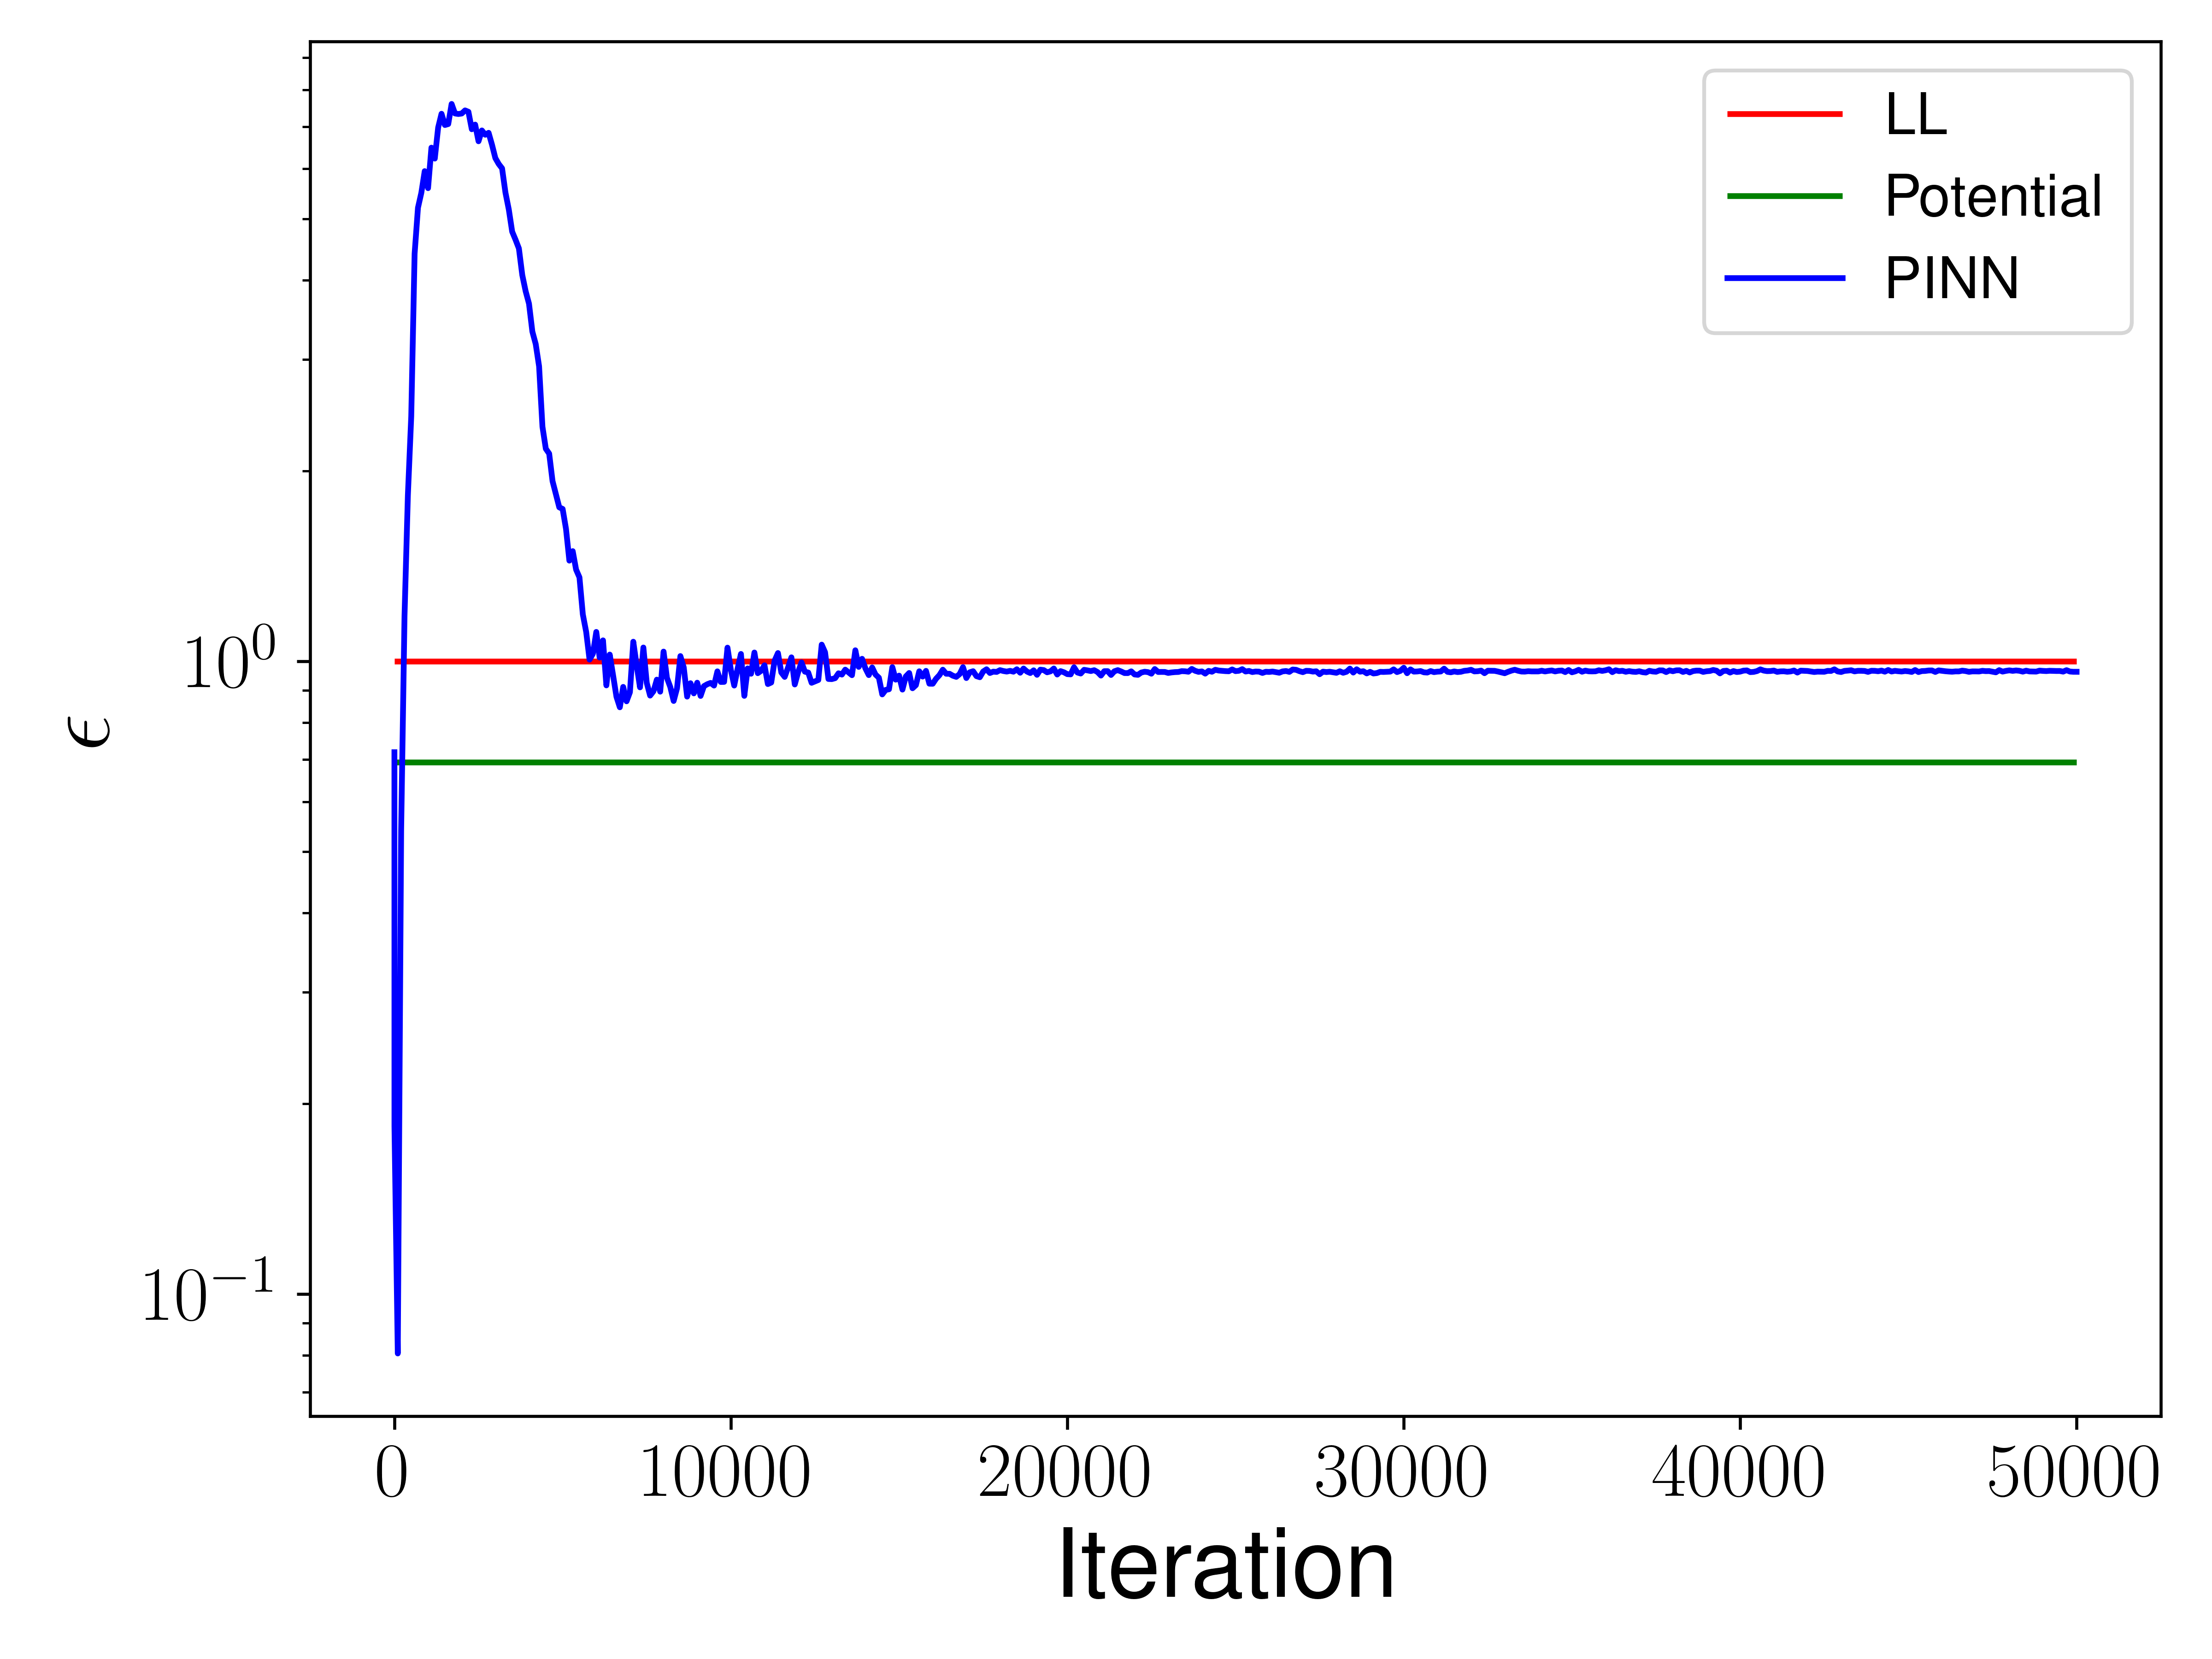
\includegraphics[width=\linewidth]{"img/graph/epsilon_ylog.png"}
    % \caption{The weighted loss of the force-free condition.}
  \end{subfigure}%
  \begin{subfigure}{.5\linewidth}
    \centering
    \caption{$\epsilon_p$}
    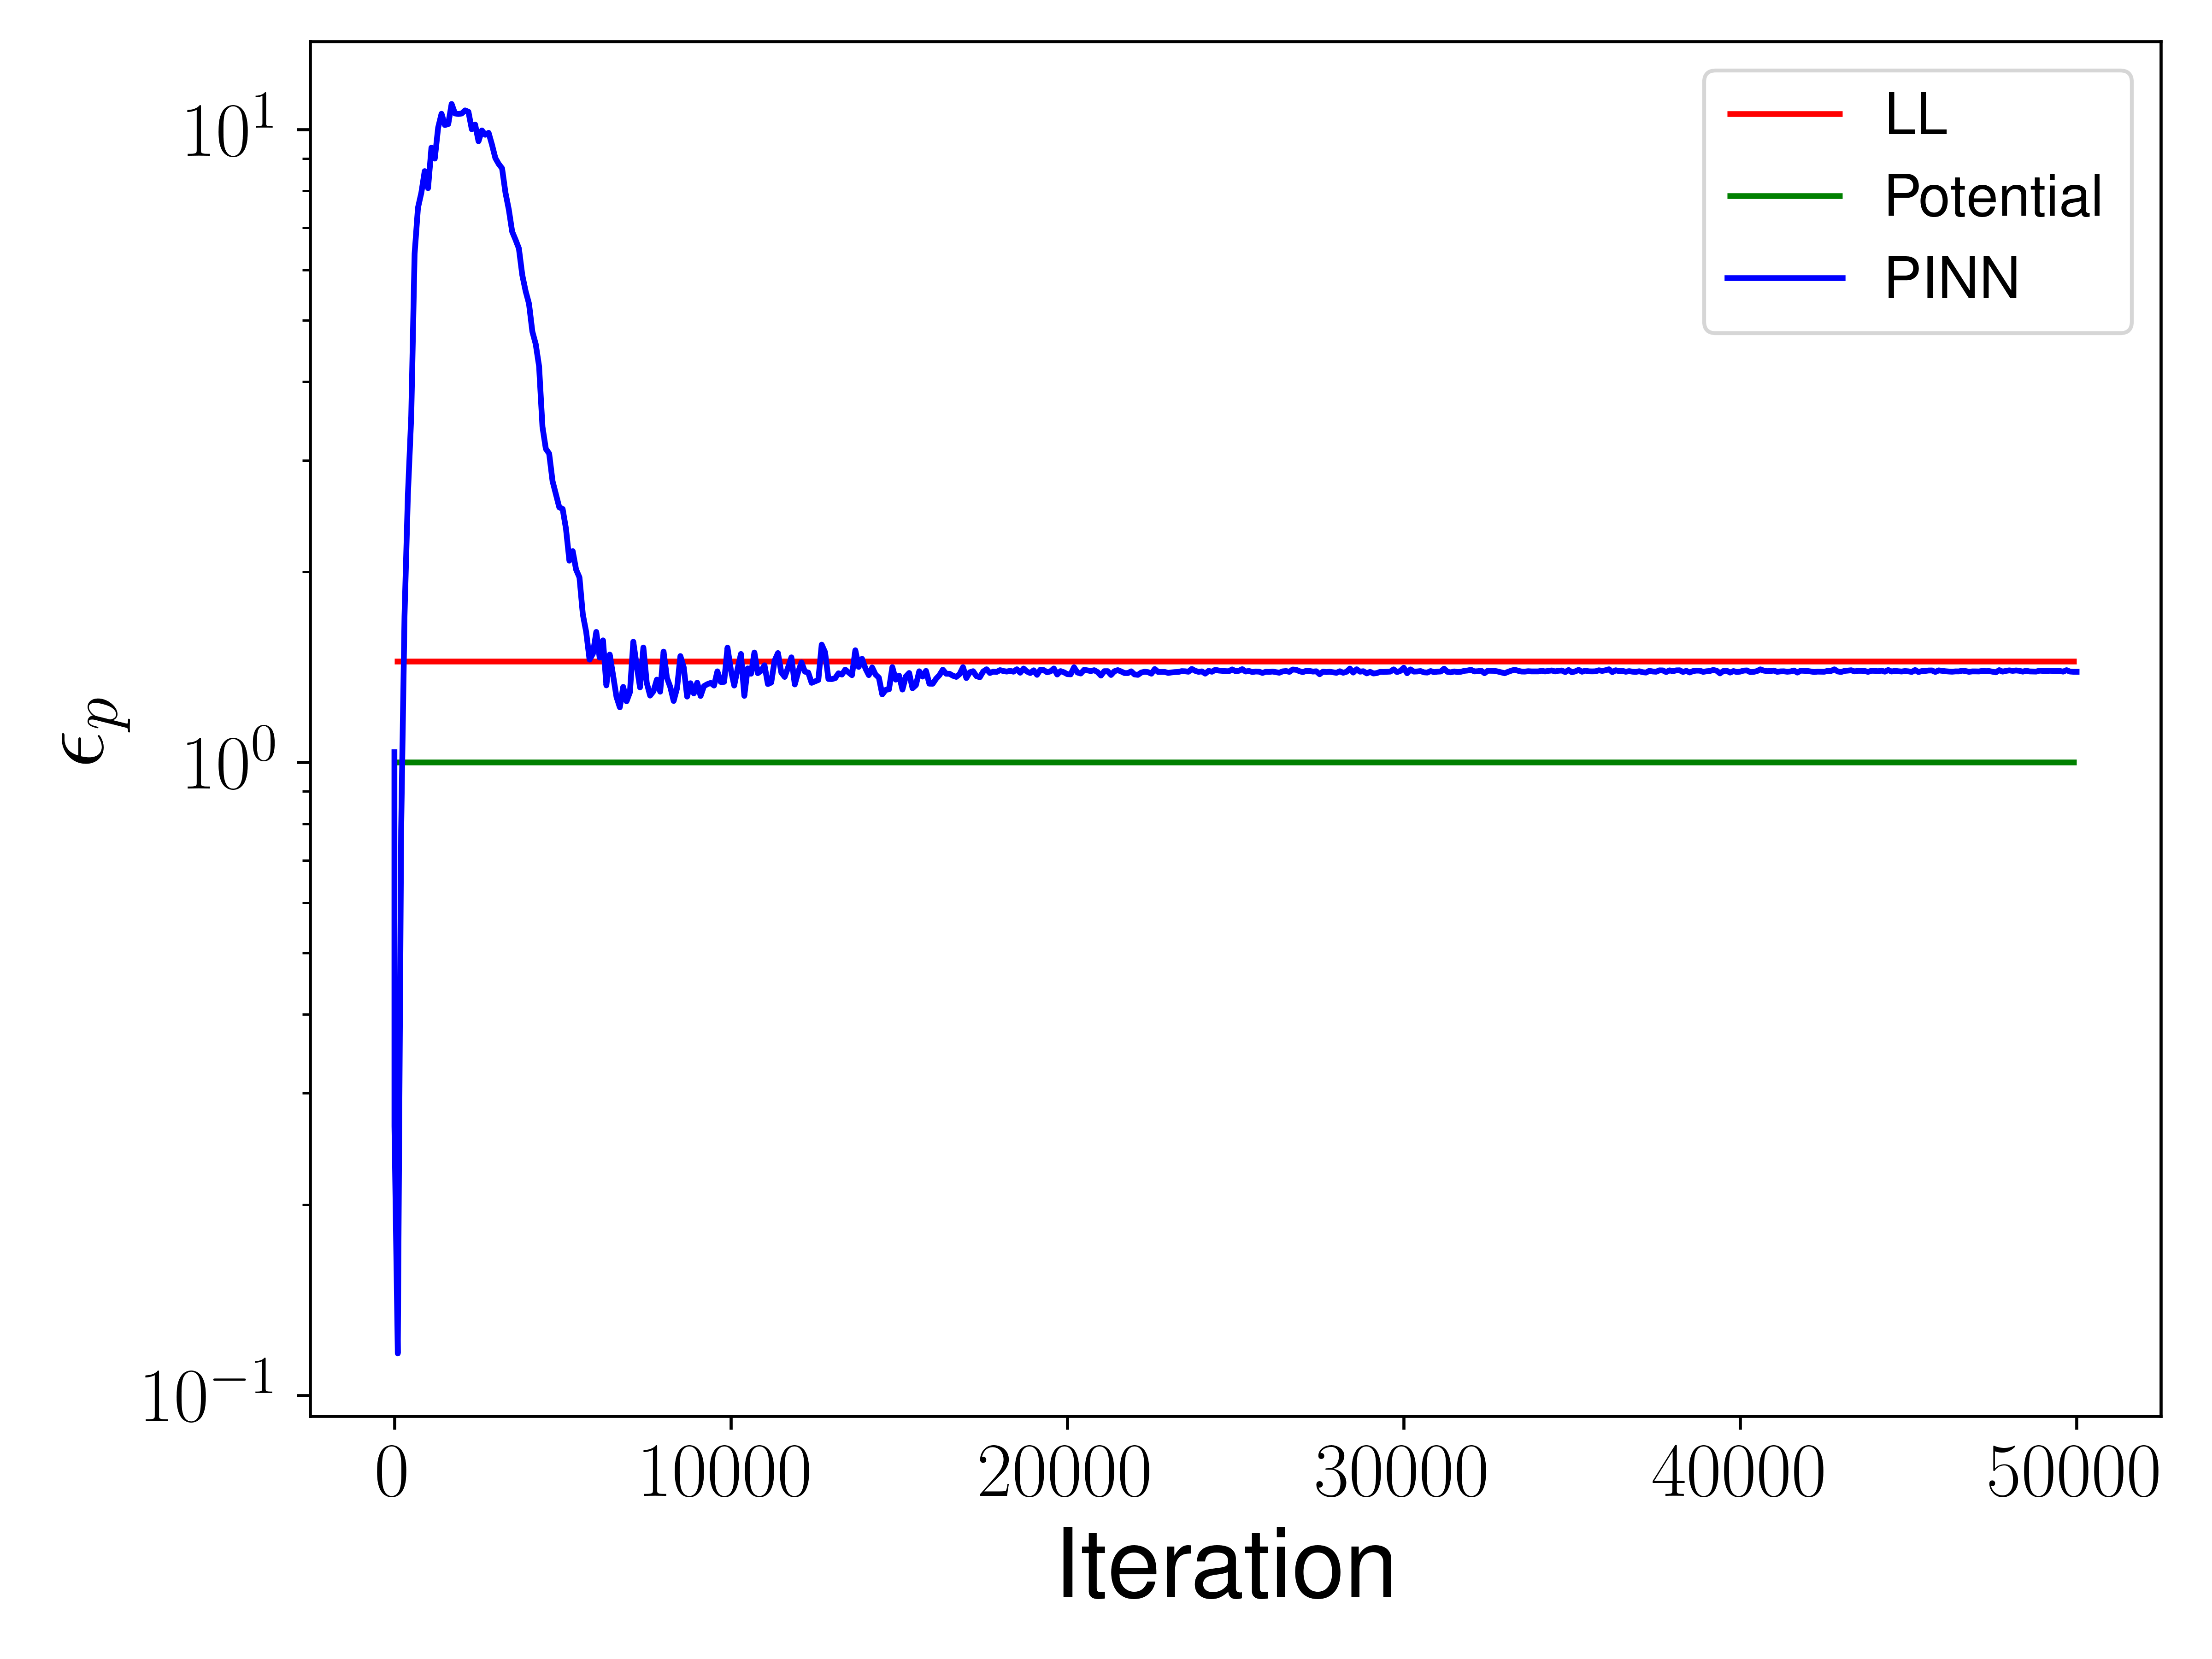
\includegraphics[width=\linewidth]{"img/graph/epsilon_p_ylog.png"}
    % \caption{The weighted loss of the solenoidal condition.}
  \end{subfigure}

  \begin{subfigure}{.5\linewidth}
    \centering
    \caption{$\text{CW}_\text{sin}$}
    \includegraphics[width=\linewidth]{"img/graph/CW_{text{sin}}.png"}
    % \caption{The weighted loss of the force-free condition.}
  \end{subfigure}%
  \begin{subfigure}{.5\linewidth}
    \centering
    \caption{$\mathcal{L}$}
    \includegraphics[width=\linewidth]{"img/graph/mathcal{L}_ylog.png"}
    % \caption{The weighted loss of the solenoidal condition.}
  \end{subfigure}

  \caption{The figures of metrit and total loss of PINN with respect to the iteration steps. The red denotes Low-Lou (LL) model, the green denotes the potential field calulated using that LL model, and the blue denotes the magnetic field reconstructed by PINN. The y-axes of the graphs for $\epsilon$, $\epsilon_p$, and $\mathcal{L}$ are in a base-10 logarithmic scale.}\label{fig:metric}
\end{figure}

In the expressions of the figures of merit, the variable $i$ represents each individual point within the computational domain, $M$ corresponds to the total number of points in the computational domain, $\mathbf{B}_{\text{p}}$ is the potential magnetic field whose bottom boundary condition is the same as that of $\mathbf{B}$, and $\mathbf{J} = \nabla \times \mathbf{B}$ is the current density in an appropriate unit system. The vector correlation metric $C_\text{vec}$ serves as a correlation coefficient specifically designed for vector fields. It has a value of $1$ when the vectors $\mathbf{B}$ and $\mathbf{b}$ are identical, and $0$ when $\mathbf{B}_i$ is perpendicular to $\mathbf{b}_i$ at each point. The Cauchy-Schwartz metric $C_\text{CS}$ quantifies the angles between vector fields. For $\mathbf{B}$ and $\mathbf{b}$ that are parallel, $C_\text{CS}$ equals $1$, while it becomes $-1$ for an anti-parallel case. When $\mathbf{B}_i$ is perpendicular to $\mathbf{b}_i$ at each point, $C_\text{CS}$ has a value of $0$. To measure the disparities between vector fields, the normalized and mean vector error metrics, $E_n$ and $E_m$ respectively, are employed. Both $E_n$ and $E_m$ are set to $0$ when $\mathbf{B}$ and $\mathbf{b}$ are identical. Since only these two metrics yield zero for a perfect match between $\mathbf{B}$ and $\mathbf{b}$, it is common to use $E'_n=1-E_n$ and $E'_m=1-E_m$ instead. Throughout this thesis, I have utilized $E'_n$ and $E'_m$. The total magnetic energy ratio, denoted as $\epsilon$, represents the ratio between the total magnetic energy of the two vector fields, $\mathbf{B}$ and $\mathbf{b}$. When $\mathbf{B}$ and $\mathbf{b}$ are identical, $\epsilon$ equals $1$.  Hence, if the physics-informed neural network method accurately reconstructs the Low-Lou analytical solution, all five metrics—$C_\text{vec}$, $C_\text{CS}$, $E'_n$, $E'_m$, and $\epsilon$—will be equal to $1$.

Considering that the potential field represents the state of lowest possible energy of any force-free fields with the same boundary condition, the magnetic energy of a nonlinear force-free field always surpasses that of the potential field. The surplus energy is known as free magnetic energy, which characterizes the energy associated with solar activities. The ratio $\epsilon_p$ between the total magnetic energy and the potential field energy indicates the amount of free magnetic energy stored in the nonlinear force-free field. For any field other than the potential field, $\epsilon_p$ exceeds $1$. The current-weighted sine metric, denoted as $\text{CW}_\text{sin}$, serves as an indicator of the force-freeness of the calculated magnetic field $\mathbf{B}$. When $\mathbf{B}$ is an exact force-free field, $\text{CW}_\text{sin}$ equals $0$. However, this metric, $\text{CW}_\text{sin}$, cannot be defined for the potential field because it has zero current density, $\mathbf{J}=\mathbf{0}$.

%For an alternative metric, I used the ratio $\zeta$ of the magnitude of the current density,
% \begin{equation*}
%   \zeta = \frac{\sum_i |\mathbf{J}_i|}{\sum_i |\mathbf{j}_i|},
% \end{equation*}
% where $\mathbf{J} = \nabla \times \mathbf{B}$ and $\mathbf{j} = \nabla \times \mathbf{b}$: $\zeta=1$ when the fields $\mathbf{B}$ and $\mathbf{b}$ are identical, $\zeta=0$ when the field $\mathbf{B}$ is a potential field, and  $\zeta$ is small when the field $\mathbf{B}$ has small free magnetic energy compared to the reference field $\mathbf{b}$, i.e., it is similar to the metric $\epsilon_p$ but it does not use the potential field to calculate the metric.

The optimizer of PINN aims to minimize the loss function $\mathcal{L}$ in a 528,131-dimensional parameter space. As a result, the loss function of PINN does not typically exhibit a monotonic decrease with respect to the iteration steps, as shown in \cref{fig:loss}. Although all the losses generally exhibit a monotonically decreasing trend after reaching certain critical points, the presence of numerous spikes in the graph indicates the challenges posed by the high-dimensionality of the parameter space. Initially, due to the high value of the boundary condition weight $w_b$ (starting from 1000), the weighted boundary condition loss $w_b\mathcal{L}_b$ dominates the total loss. Subsequently, as the boundary condition weight $w_b$ exponentially decreases, the weighted PDE losses $w_\text{ff}\mathcal{L}_\text{ff}$ and $w_\text{div}\mathcal{L}_\text{div}$ become increasingly influential in the total loss. In that time, they already has the decreasing pattern like the BC loss. Therefore, the overall pattern of the total loss closely resembles that of the boundary condition loss. 

The force-free condition loss $\mathcal{L}_\text{ff}$ and the solenoidal condition loss $\mathcal{L}_\text{div}$ display patterns of both increase and decrease. This behavior can be attributed to the fact that the initial field generated randomly for PINN, in this case, is a nearly constant vector field, as depicted in (a) of \cref{fig:xy,fig:yz,fig:xz,fig:xz_tilted}. Consequently, the derivatives of the initial magnetic field are close to zero, resulting in nearly zero PDE losses $\mathcal{L}_\text{ff}$ and $\mathcal{L}_\text{div}$.

As the training progresses, the field reconstructed by PINN satisfies the boundary conditions at $\partial V$, but it may not adhere to the force-free condition and solenoidal condition due to the initially high boundary condition weight $w_b$. Once the weighted boundary condition loss decreases sufficiently, the optimizer focuses on minimizing the PDE losses within the volume $V$, which now constitute the majority of the total loss. Consequently, the field gradually evolves into a nonlinear force-free field that satisfies the prescribed boundary conditions while simultaneously reducing the PDE losses. 

Although the primary objective of the optimizer is to minimize the total loss $\mathcal{L}$, the seven metrics ($C_\text{vec}$, $C_\text{CS}$, $E'_n$, $E'_m$, $\epsilon$, $\epsilon_p$, and $\text{CW}_\text{sin}$) of the PINN-reconstructed magnetic field closely resemble those of the Low-Lou model, as depicted in \cref{fig:metric}. This observation confirms that the loss function employed in traditional optimization methods can also be utilized in the PINN approach, demonstrating the ability of the physics-informed neural network method to reconstruct nonlinear force-free fields. It is worth noting that the PINN-reconstructed solution surpasses the potential field as it exhibits closer proximity to the Low-Lou analytical solution.

However, while $\mathcal{L}$ serves as a valuable loss function, it is not flawless. As shown in \cref{tab:metric}, the figures of merit ($C_\text{vec}$, $E'_n$, $E'_m$, $\epsilon$, and $\epsilon_p$) for the PINN(50000) model are inferior (deviating from the values of the Low-Lou model) compared to those of the PINN(25000) model, even though $\mathcal{L}$ decreases from 0.00006 to 0.00005. Meanwhile, $C_\text{CS}$ and $\text{CW}_\text{sin}$ for the PINN(50000) model outperform those of the PINN(25000) model. This observation suggests the need for the development of more appropriate loss functions in future research.

Furthermore, the energy metrics $\epsilon$ and $\epsilon_p$ of the PINN(50000) model exhibit lower values compared to the Low-Lou solution. This indicates that the total magnetic energy and free magnetic energy of the PINN(50000) model are smaller than those of the Low-Lou solution. This finding may imply the presence of spectral bias in the PINN method \parencite{rahaman2019spectral}, i.e., the neural network tends to prioritize learning low-frequency features while facing challenges with high-frequency features. Actually, a smooth distribution of magnetic fields, favored by the PINN approach, typically results in lower magnetic energy compared to a more spiky distribution because of the squaring operation in the definition of magnetic energy $\int_{V} \frac{B^2}{8\pi} \mathrm{d}V$: $8 = 2^2 + 2^2 < 3^2 + 1^2 = 10$.

The colors in the $z=0$ plane in the \cref{fig:xy,fig:yz,fig:xz,fig:xz_tilted} follows the typical convention for solar magnetograms: white represents positive $B_z$ values, while black represents negative $B_z$ values. All figures share the same scalar bar, which spans a range of (-150, 150). Additionally, 25 field lines have been selected, and each field line is assigned a unique color to distinguish it from the others. The colors are randomly assigned based on the seed value calculated from the coordinates of the field line's starting point. Thus, the field lines originating from the same point have the same color across all figures. These figures demonstrate that the PINN method successfully reconstructs the nonlinear force-free fields described by the Low-Lou model in qualitative terms. Furthermore, PINN(0) in these figures highlight that PINN does not require any pre-calculated initial field, such as a potential field, as is typically needed in traditional optimization methods.

\begin{table*}
  \centering
  \caption{Figures of merit for various fields and total loss of PINN. The reference field is the Low-Lou model with $(n=1, m=1, l=0.3, \Phi=\pi/2)$. PINN($i$) refers to the magnetic field calculated using PINN at the iteration step $i$.}\label{tab:metric}
  \begin{NiceTabular}{ccccccccc}
  \toprule
  Field & $C_\text{vec}$ & $C_\text{CS}$ & $E'_n$ & $E'_m$ & $\epsilon$ & $\epsilon_p$ & $\text{CW}_\text{sin}$ & $\mathcal{L}$\tabularnote{The total loss of PINN.} \\ 
  \midrule
  Low-Lou & 1.00000 & 1.00000 & 1.00000 & 1.00000 & 1.00000 & 1.44490 & 0.01308\tabularnote{This is not zero due to numerical grids.} & -- \\
  Potential & 0.86465 & 0.86925 & 0.43003 & 0.36242 & 0.69209 & 1.00000 & --\tabularnote{The metric $\text{CW}_\text{sin}$ is undefined for the potential field.} & -- \\
  PINN(0) & 0.07115 & 0.33540 & -1.37088 & -6.07067 & 0.71824 & 1.03779 & 0.55813 & 40.23570 \\
  PINN(100) & 0.25771 & 0.46100 & -0.00643 & -0.46701 & 0.08056 & 0.11640 & 0.76066 & 31.32017 \\
  PINN(1000) & 0.54244 & 0.32404 & -2.31914 & -6.41640 & 5.59377 & 8.08246 & 0.71701 & 6.46577 \\
  PINN(10000) & 0.98630 & 0.63065 & 0.68766 & 0.28275 & 0.96939 & 1.40068 & 0.38403 & 0.00848 \\
  PINN(25000) & 0.99402 & 0.92134 & 0.78452 & 0.55897 & 0.96481 & 1.39406 & 0.07853 & 0.00006 \\
  PINN(50000) & 0.99359 & 0.92271 & 0.77129 & 0.50928 & 0.96247 & 1.39068 & 0.06848 & 0.00005 \\
  \bottomrule
  \end{NiceTabular}
\end{table*}

\begin{figure}
  \begin{subfigure}{.5\linewidth}
    \centering
    \caption{$\mathcal{L}$}
    \includegraphics[width=\linewidth]{"img/graph/mathcal{L}_ylog.png"}
    % \caption{The total loss of PINN.}
  \end{subfigure}%
  \begin{subfigure}{.5\linewidth}
    \centering
    \caption{$w_b\mathcal{L}_b$}
    \includegraphics[width=\linewidth]{"img/graph/w_bmathcal{L}_b_ylog.png"}
    % \caption{The weighted loss of the boundary condition.}
  \end{subfigure}

  \begin{subfigure}{.5\linewidth}
    \centering
    \caption{$w_\text{ff}\mathcal{L}_\text{ff}$}
    \includegraphics[width=\linewidth]{"img/graph/w_text{ff}mathcal{L}_text{ff}_ylog.png"}
    % \caption{The weighted loss of the force-free condition.}
  \end{subfigure}%
  \begin{subfigure}{.5\linewidth}
    \centering
    \caption{$w_\text{div}\mathcal{L}_\text{div}$}
    \includegraphics[width=\linewidth]{"img/graph/w_text{div}mathcal{L}_text{div}_ylog.png"}
    % \caption{The weighted loss of the solenoidal condition.}
  \end{subfigure}

  \caption{The values of loss funtions with respect to the iteration steps. (a) The total loss of PINN. The weighted loss of (b) the boundary condition, (c) the force-free condition, and (d) the solenoidal condition. The y-axes of these graphs are in a base-10 logarithmic scale.}\label{fig:loss}
\end{figure}

\begin{figure}
  \begin{subfigure}{.5\linewidth}
    \centering
    \caption{PINN(0)}\label{fig:xy0}
    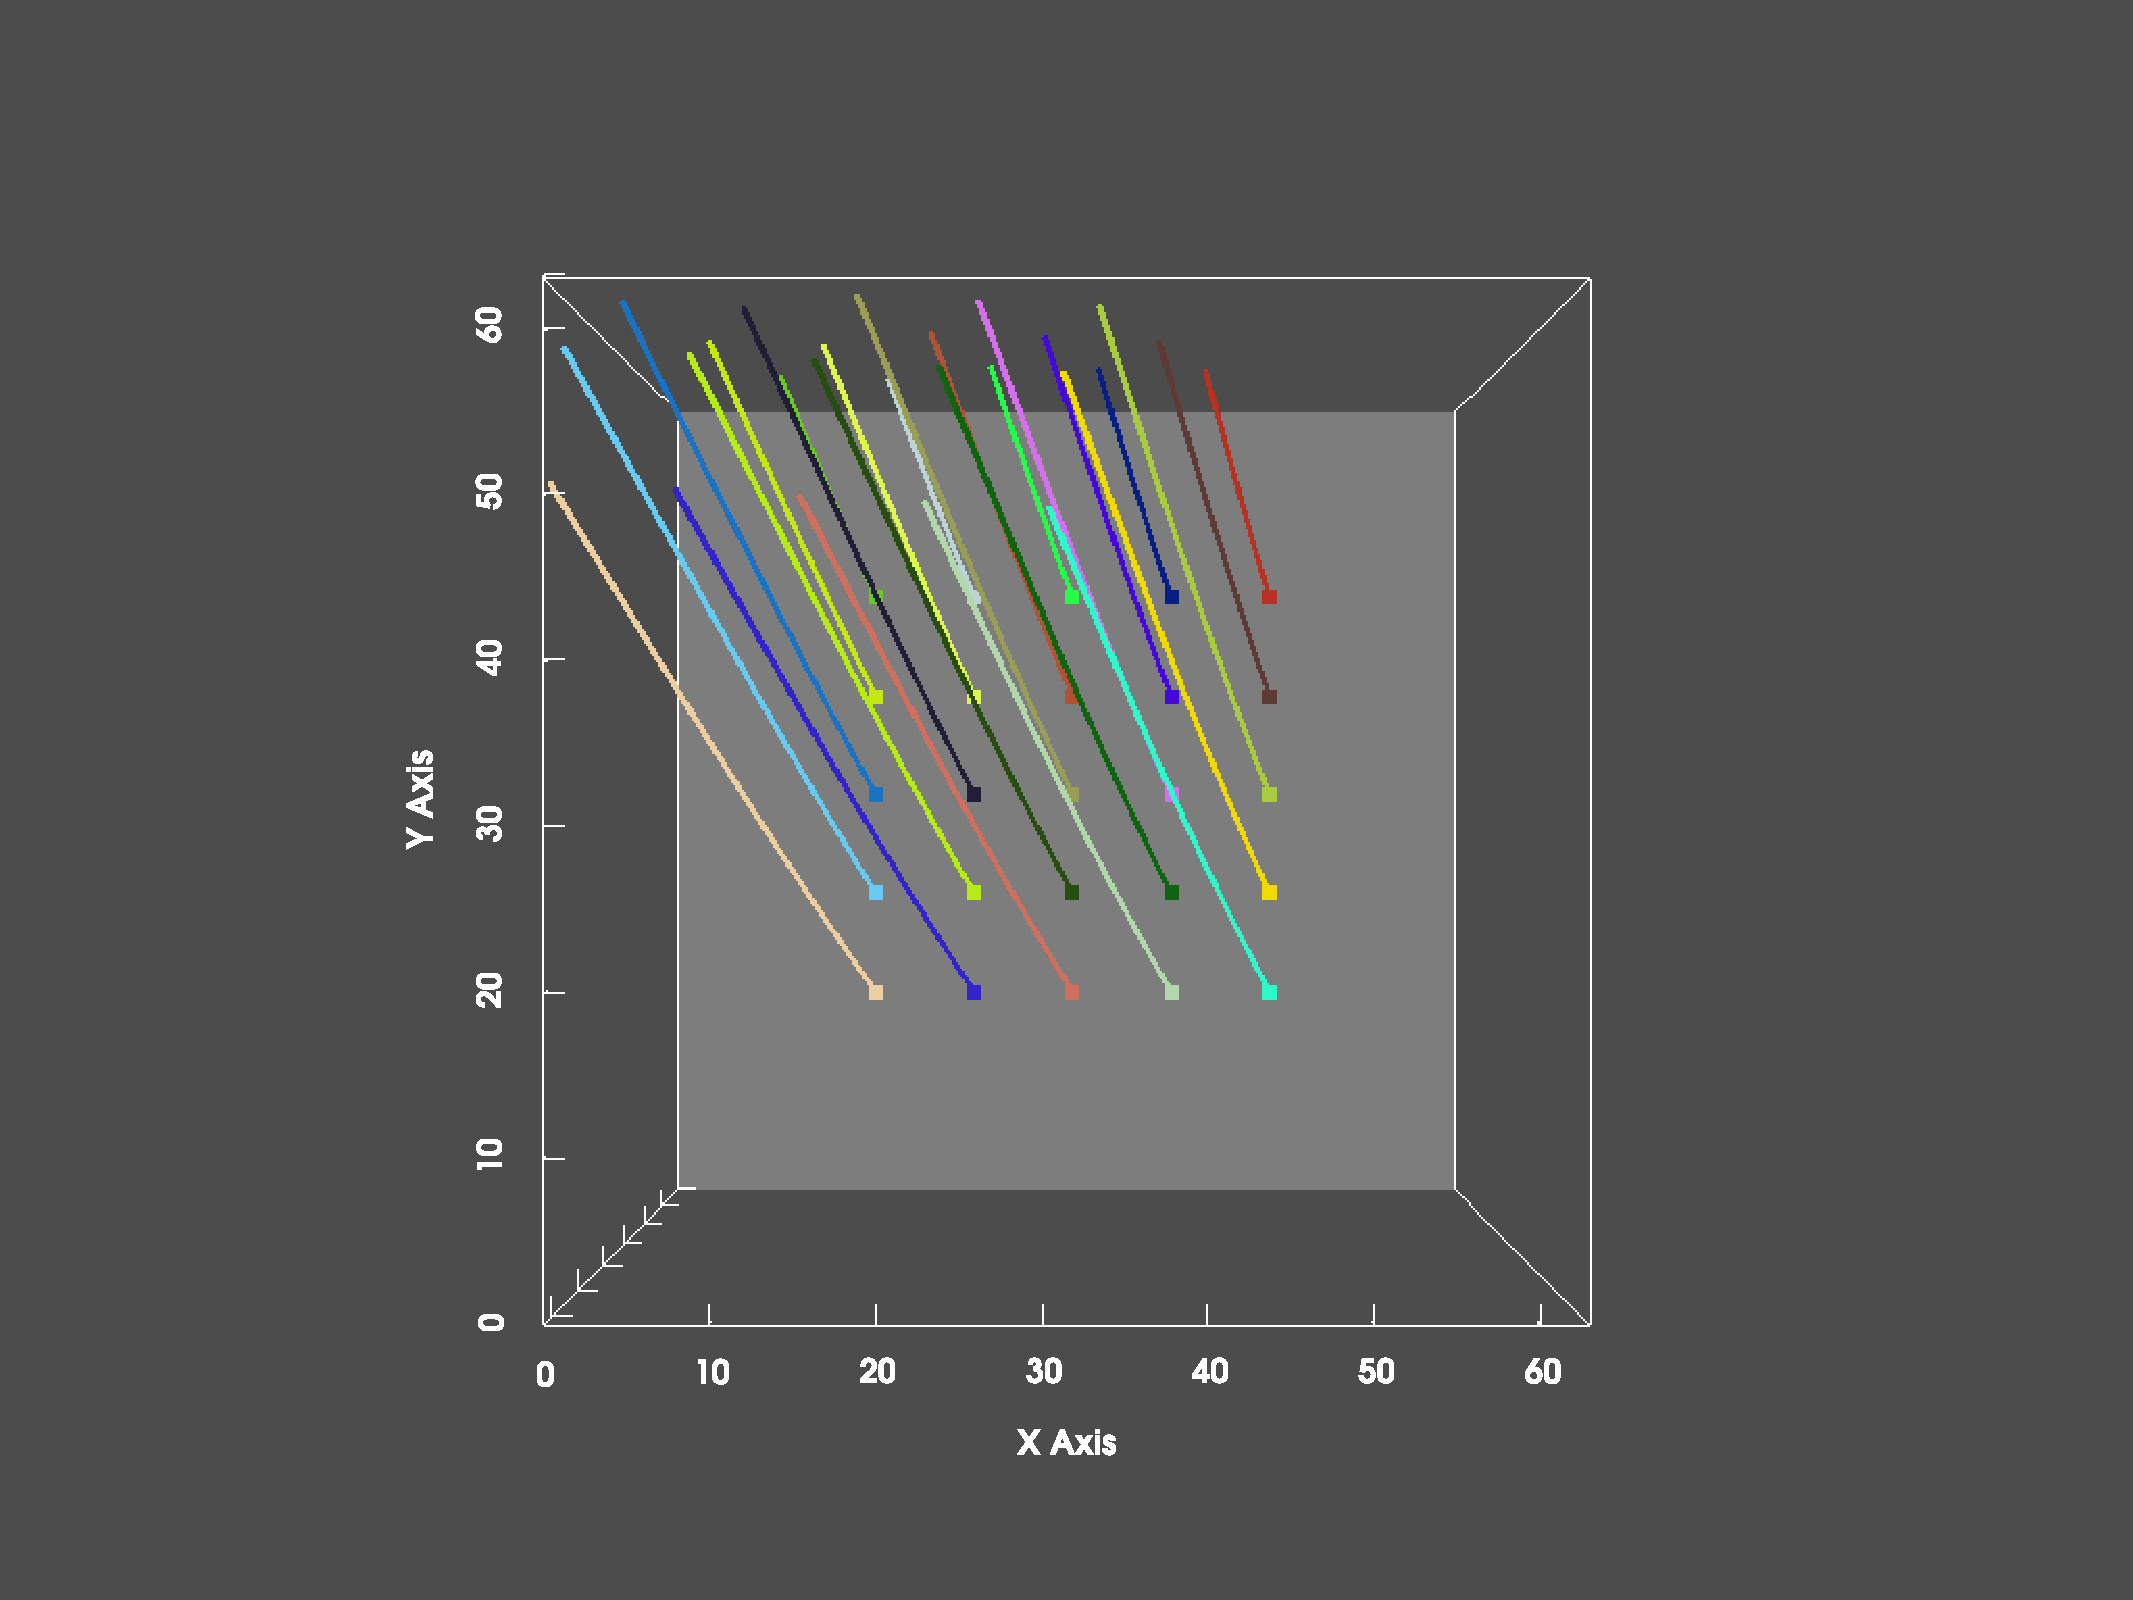
\includegraphics[trim={6cm 1cm 6cm 2cm}, clip, width=\linewidth]{"img/PINN_000000_xy.pdf"}
  \end{subfigure}%
  \begin{subfigure}{.5\linewidth}
    \centering
    \caption{PINN(100)}
    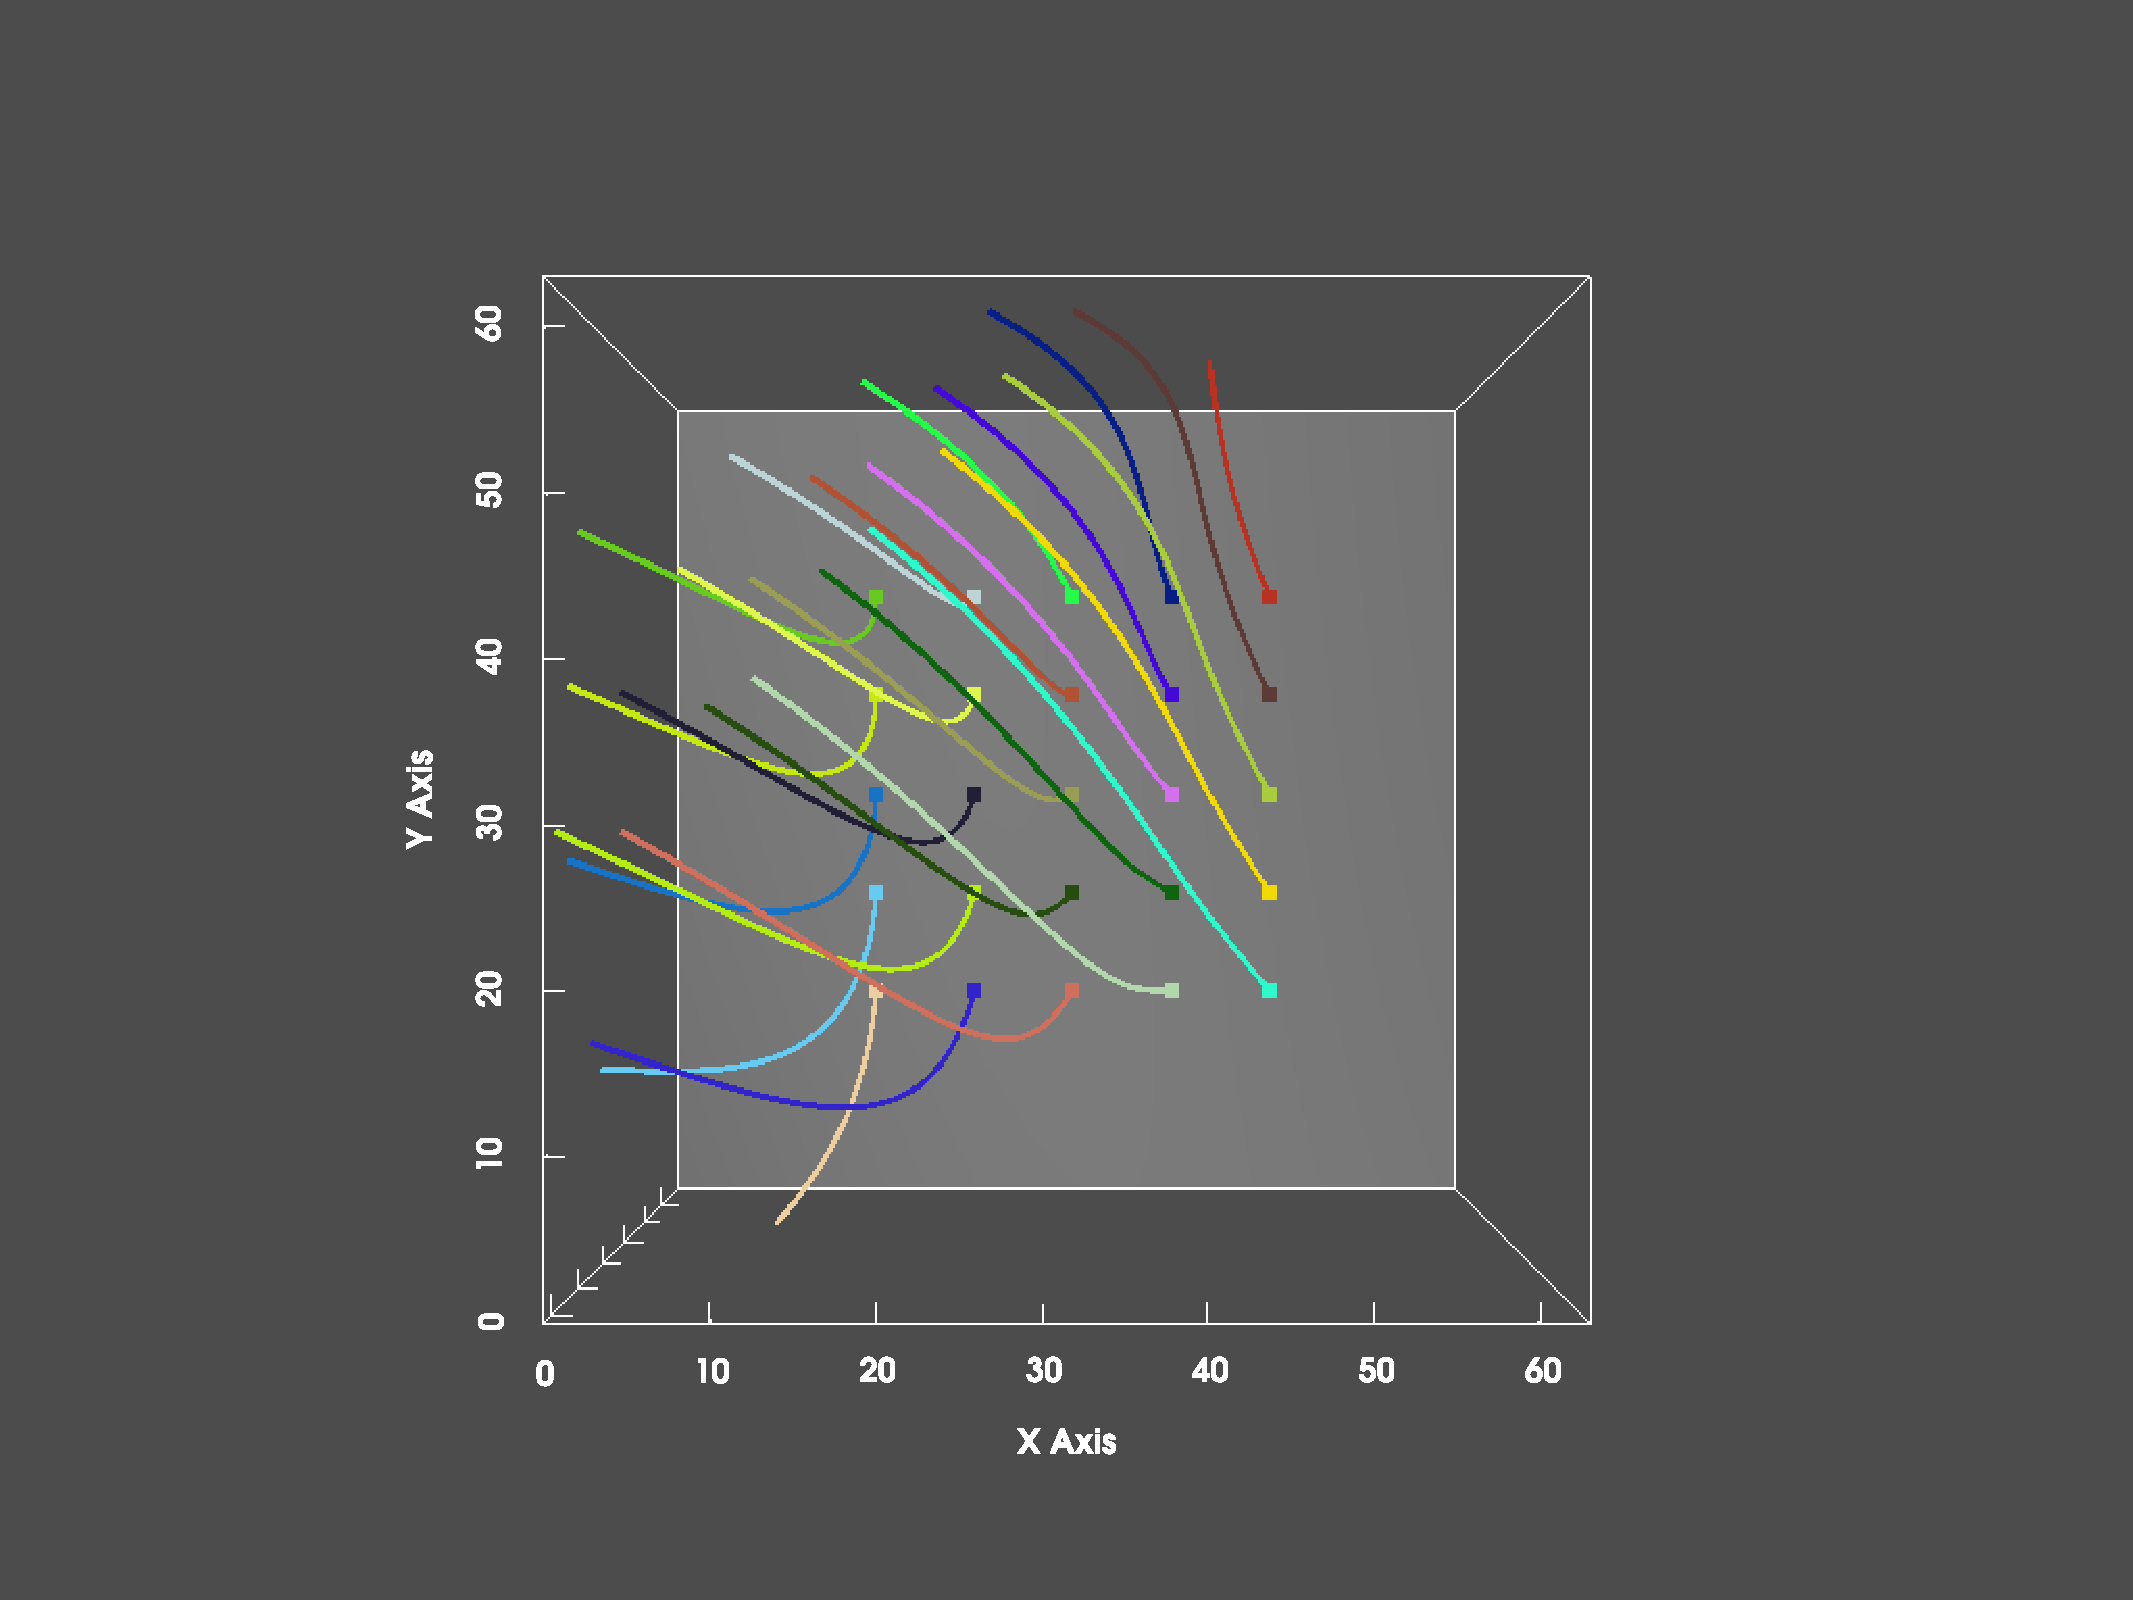
\includegraphics[trim={6cm 1cm 6cm 2cm}, clip, width=\linewidth]{"img/PINN_000100_xy.pdf"}
  \end{subfigure}

  \begin{subfigure}{.5\linewidth}
    \centering
    \caption{PINN(1000)}
    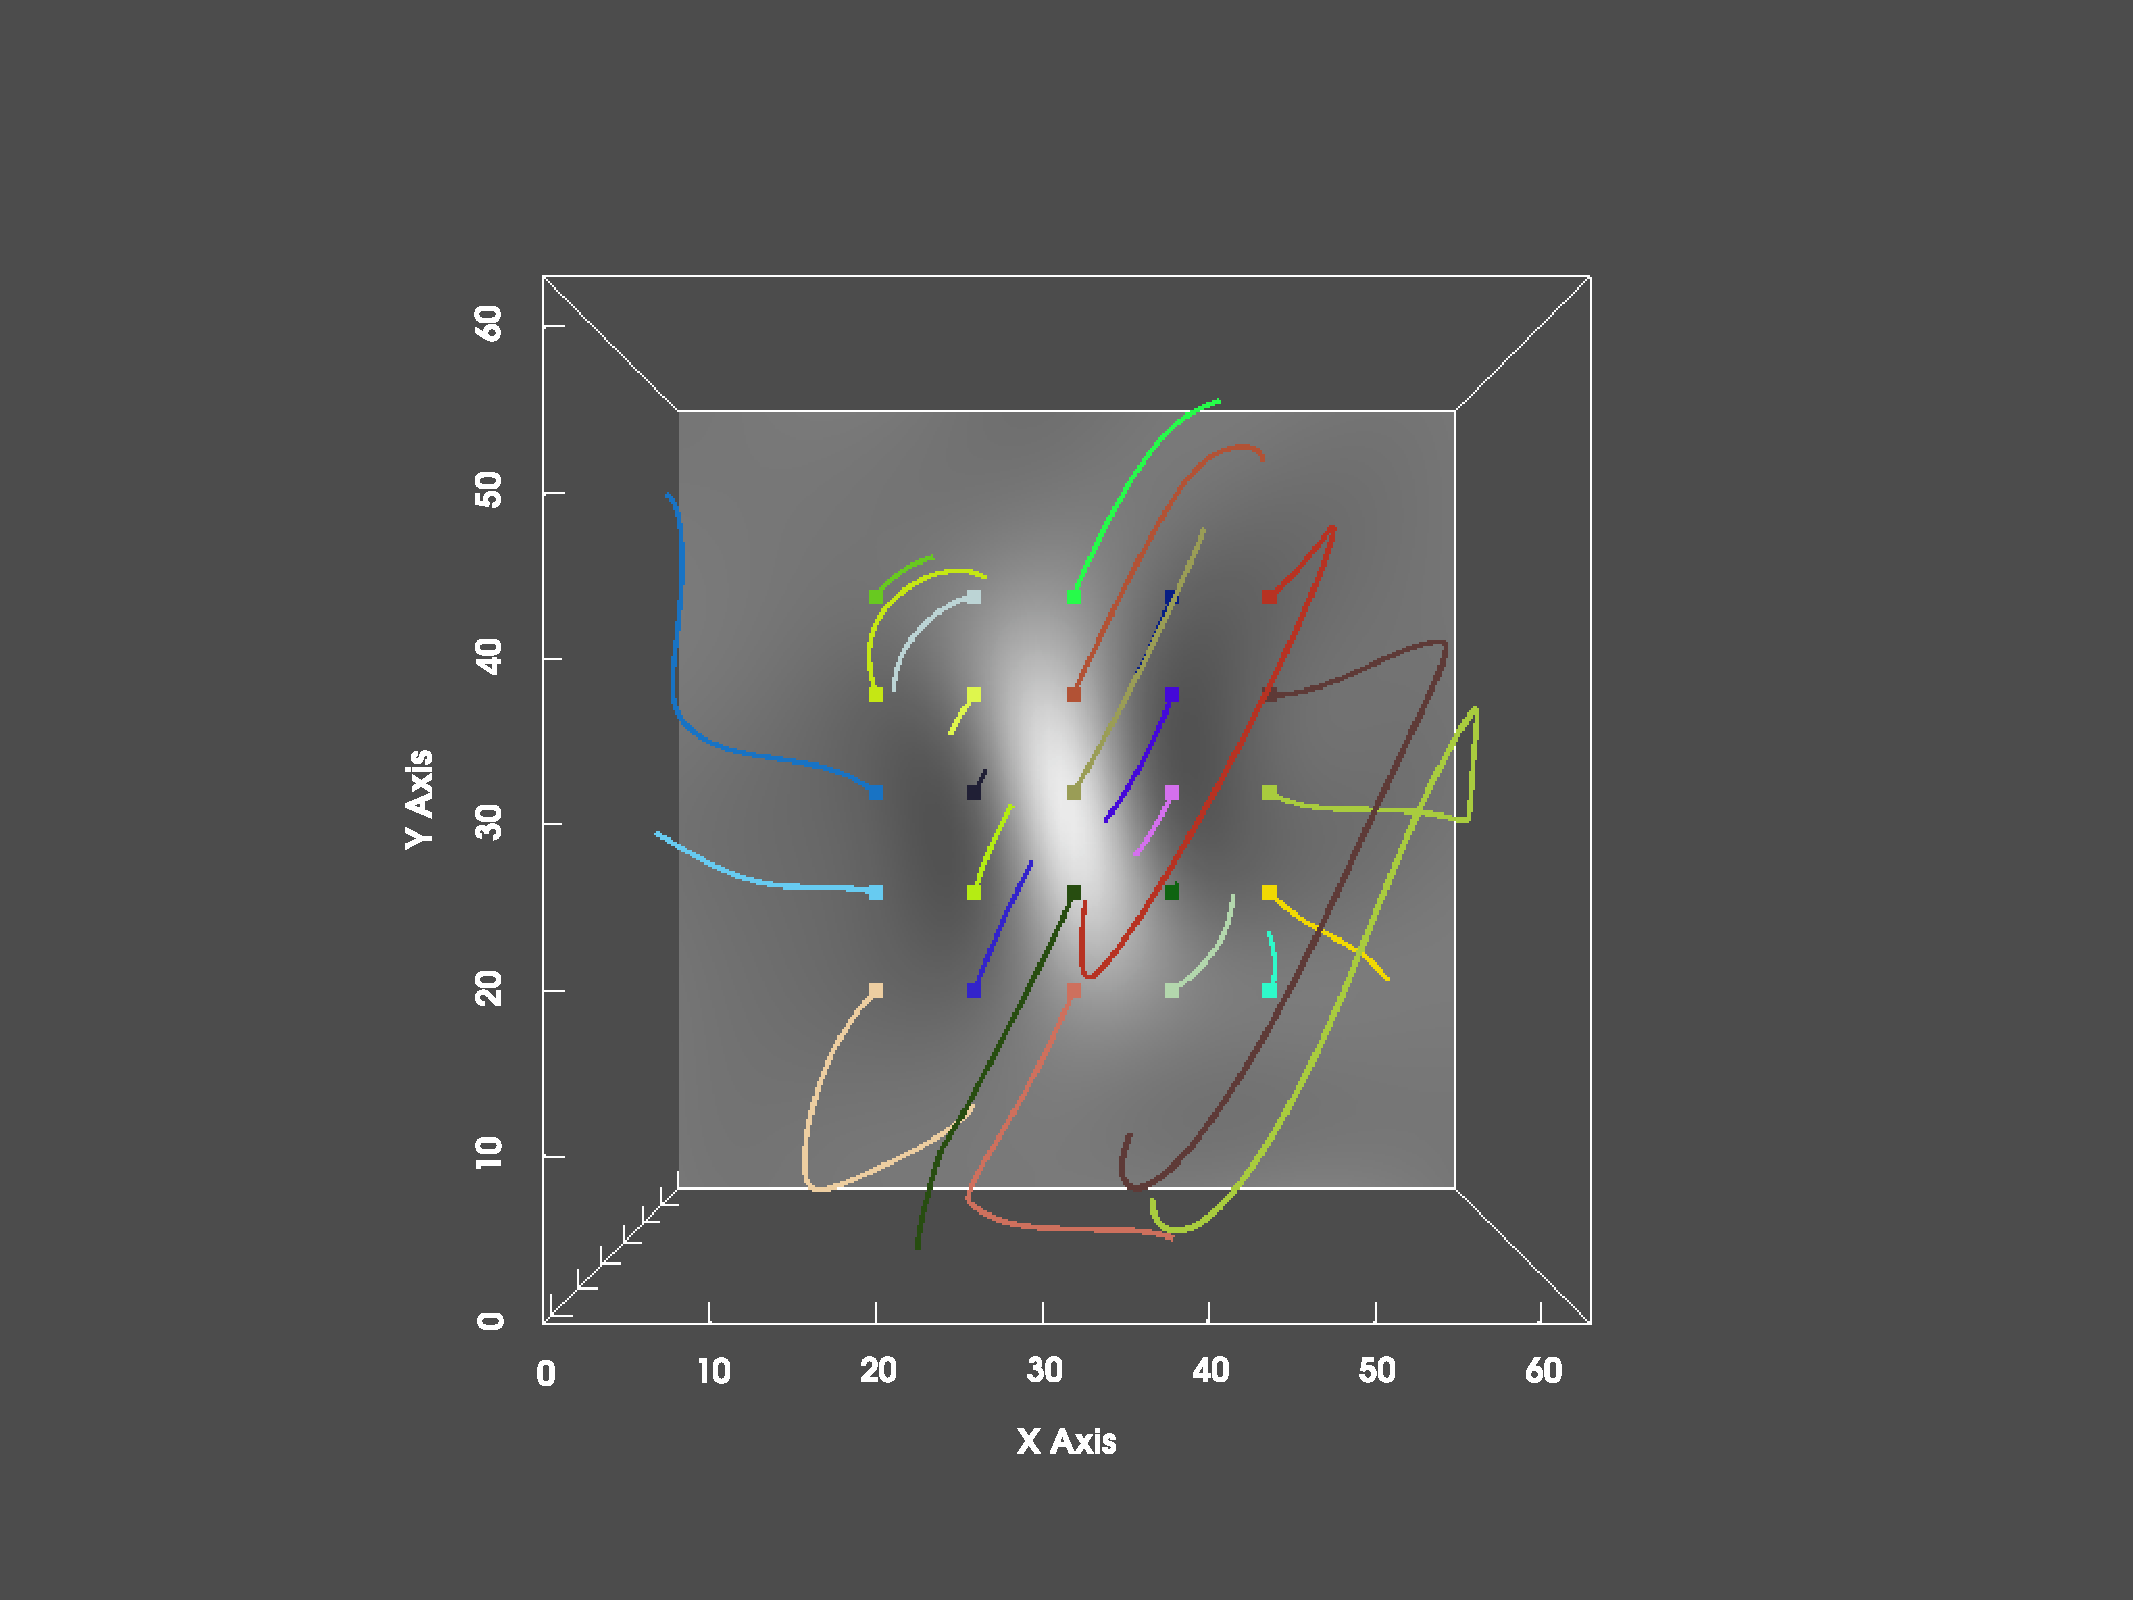
\includegraphics[trim={6cm 1cm 6cm 2cm}, clip, width=\linewidth]{"img/PINN_001000_xy.pdf"}
  \end{subfigure}%
  \begin{subfigure}{.5\linewidth}
    \centering
    \caption{PINN(10000)}
    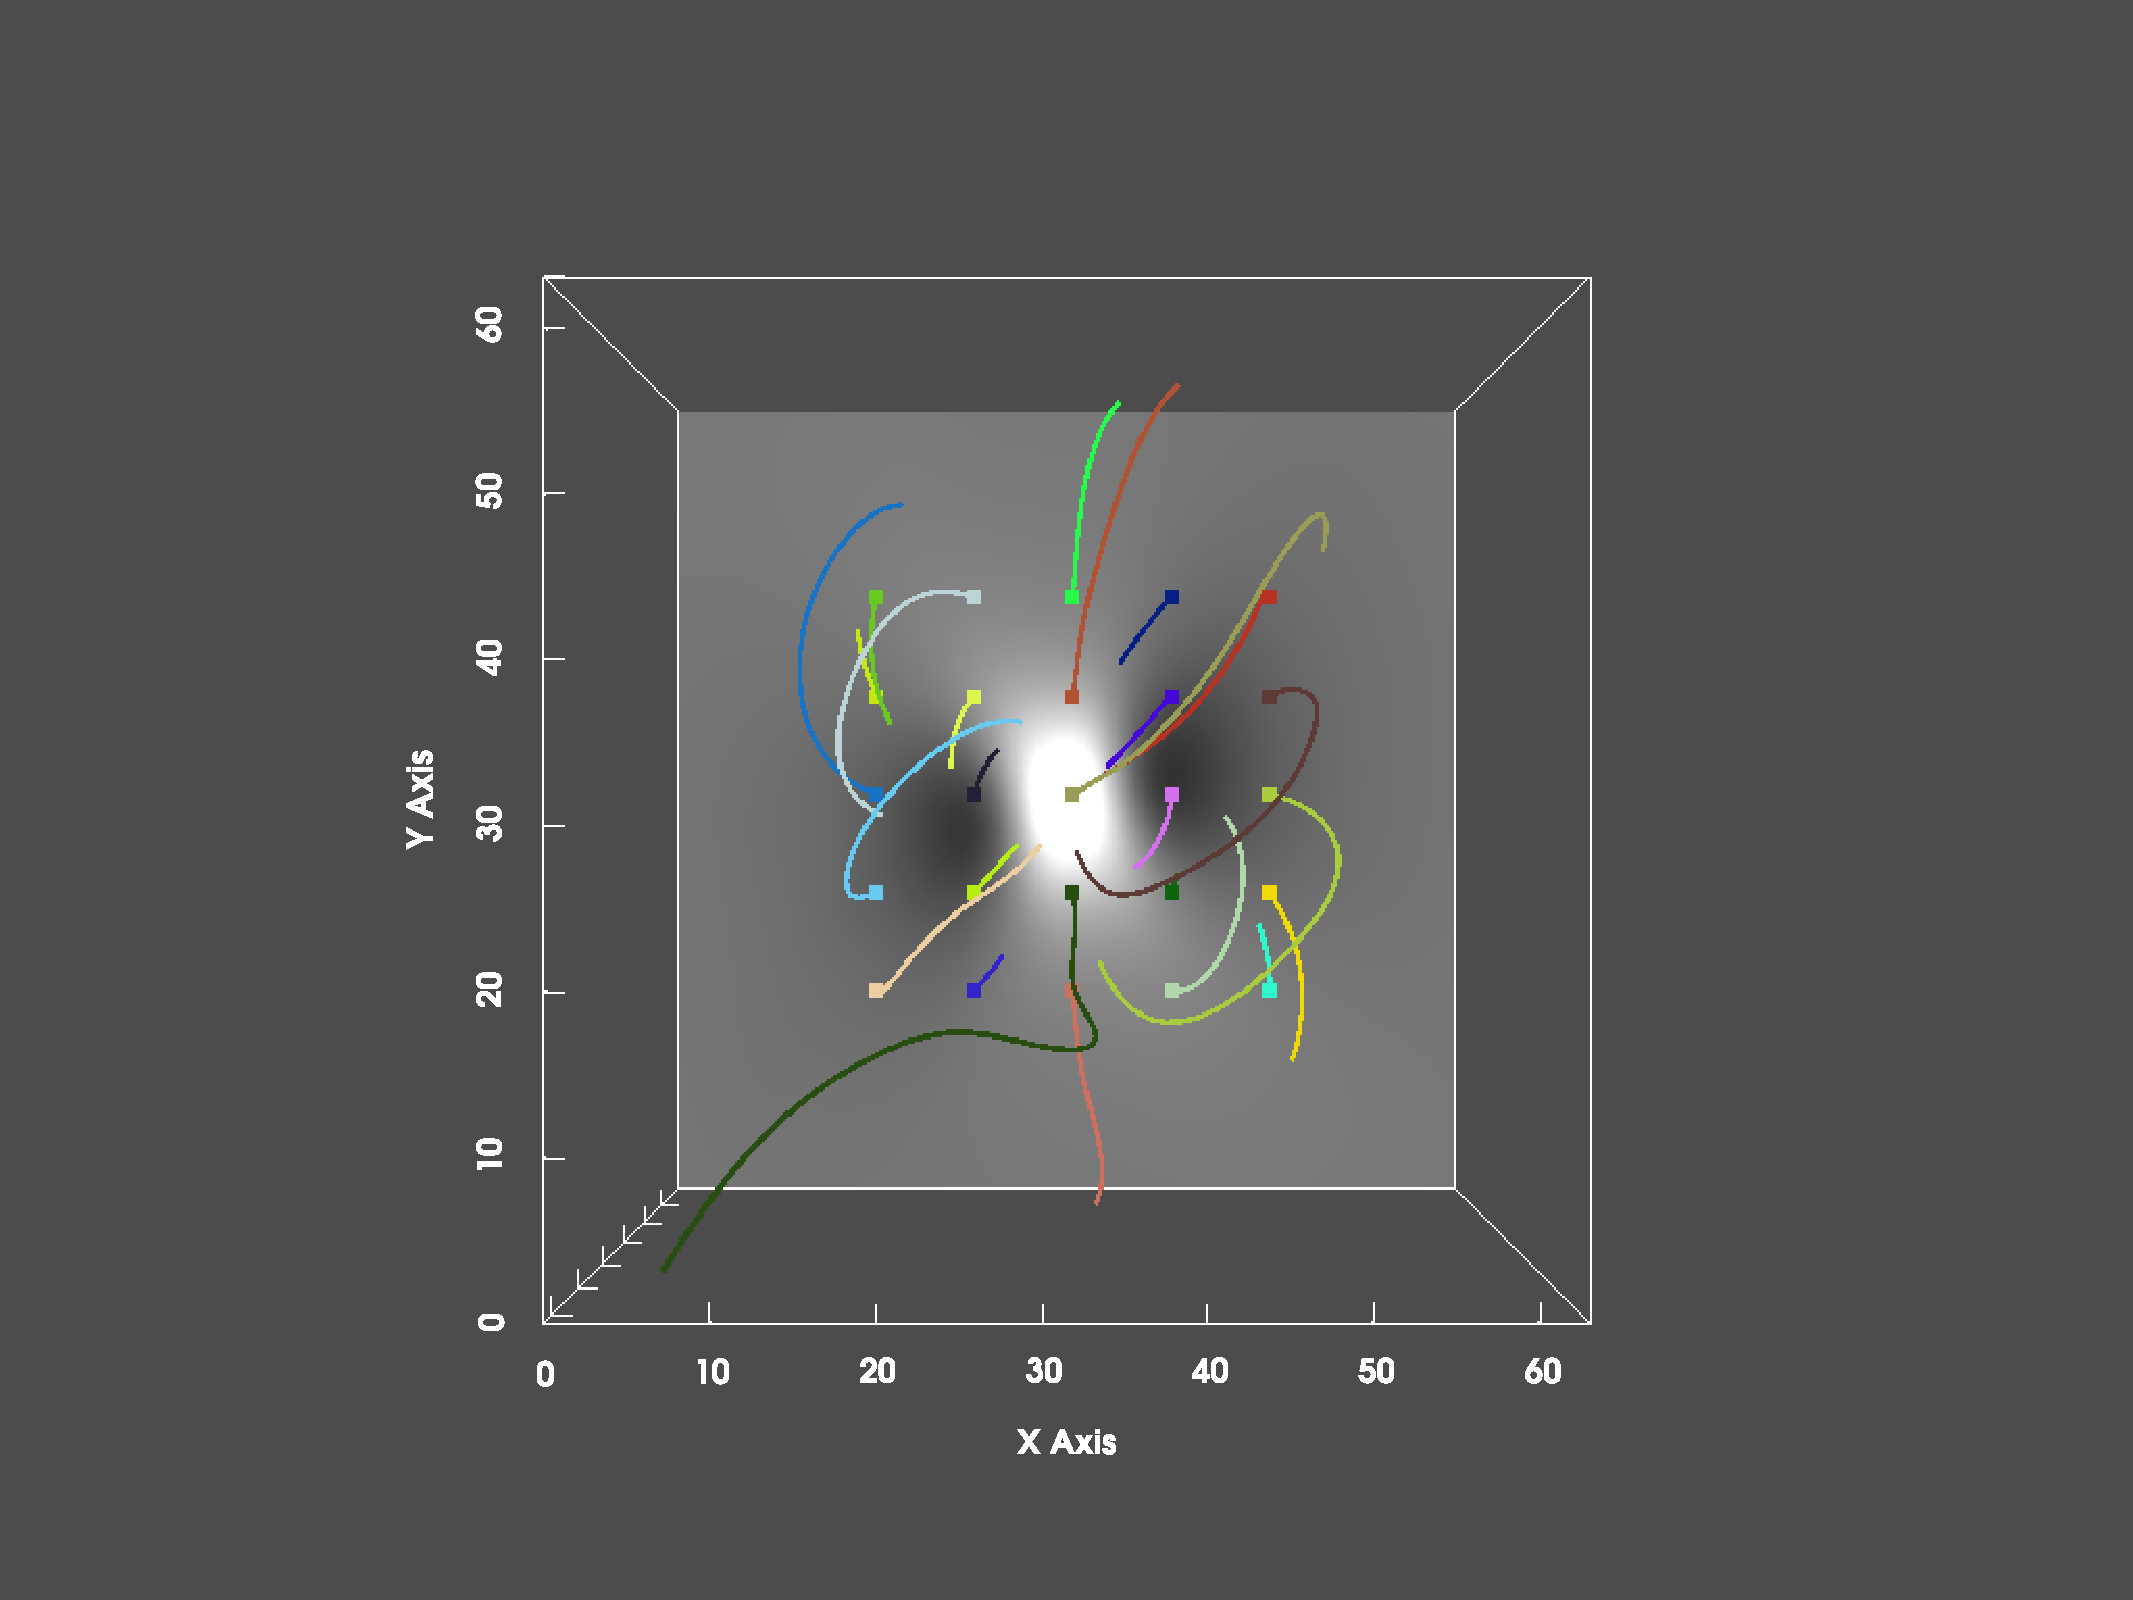
\includegraphics[trim={6cm 1cm 6cm 2cm}, clip, width=\linewidth]{"img/PINN_010000_xy.pdf"}
  \end{subfigure}

  \begin{subfigure}{.5\linewidth}
    \centering
    \caption{PINN(25000)}
    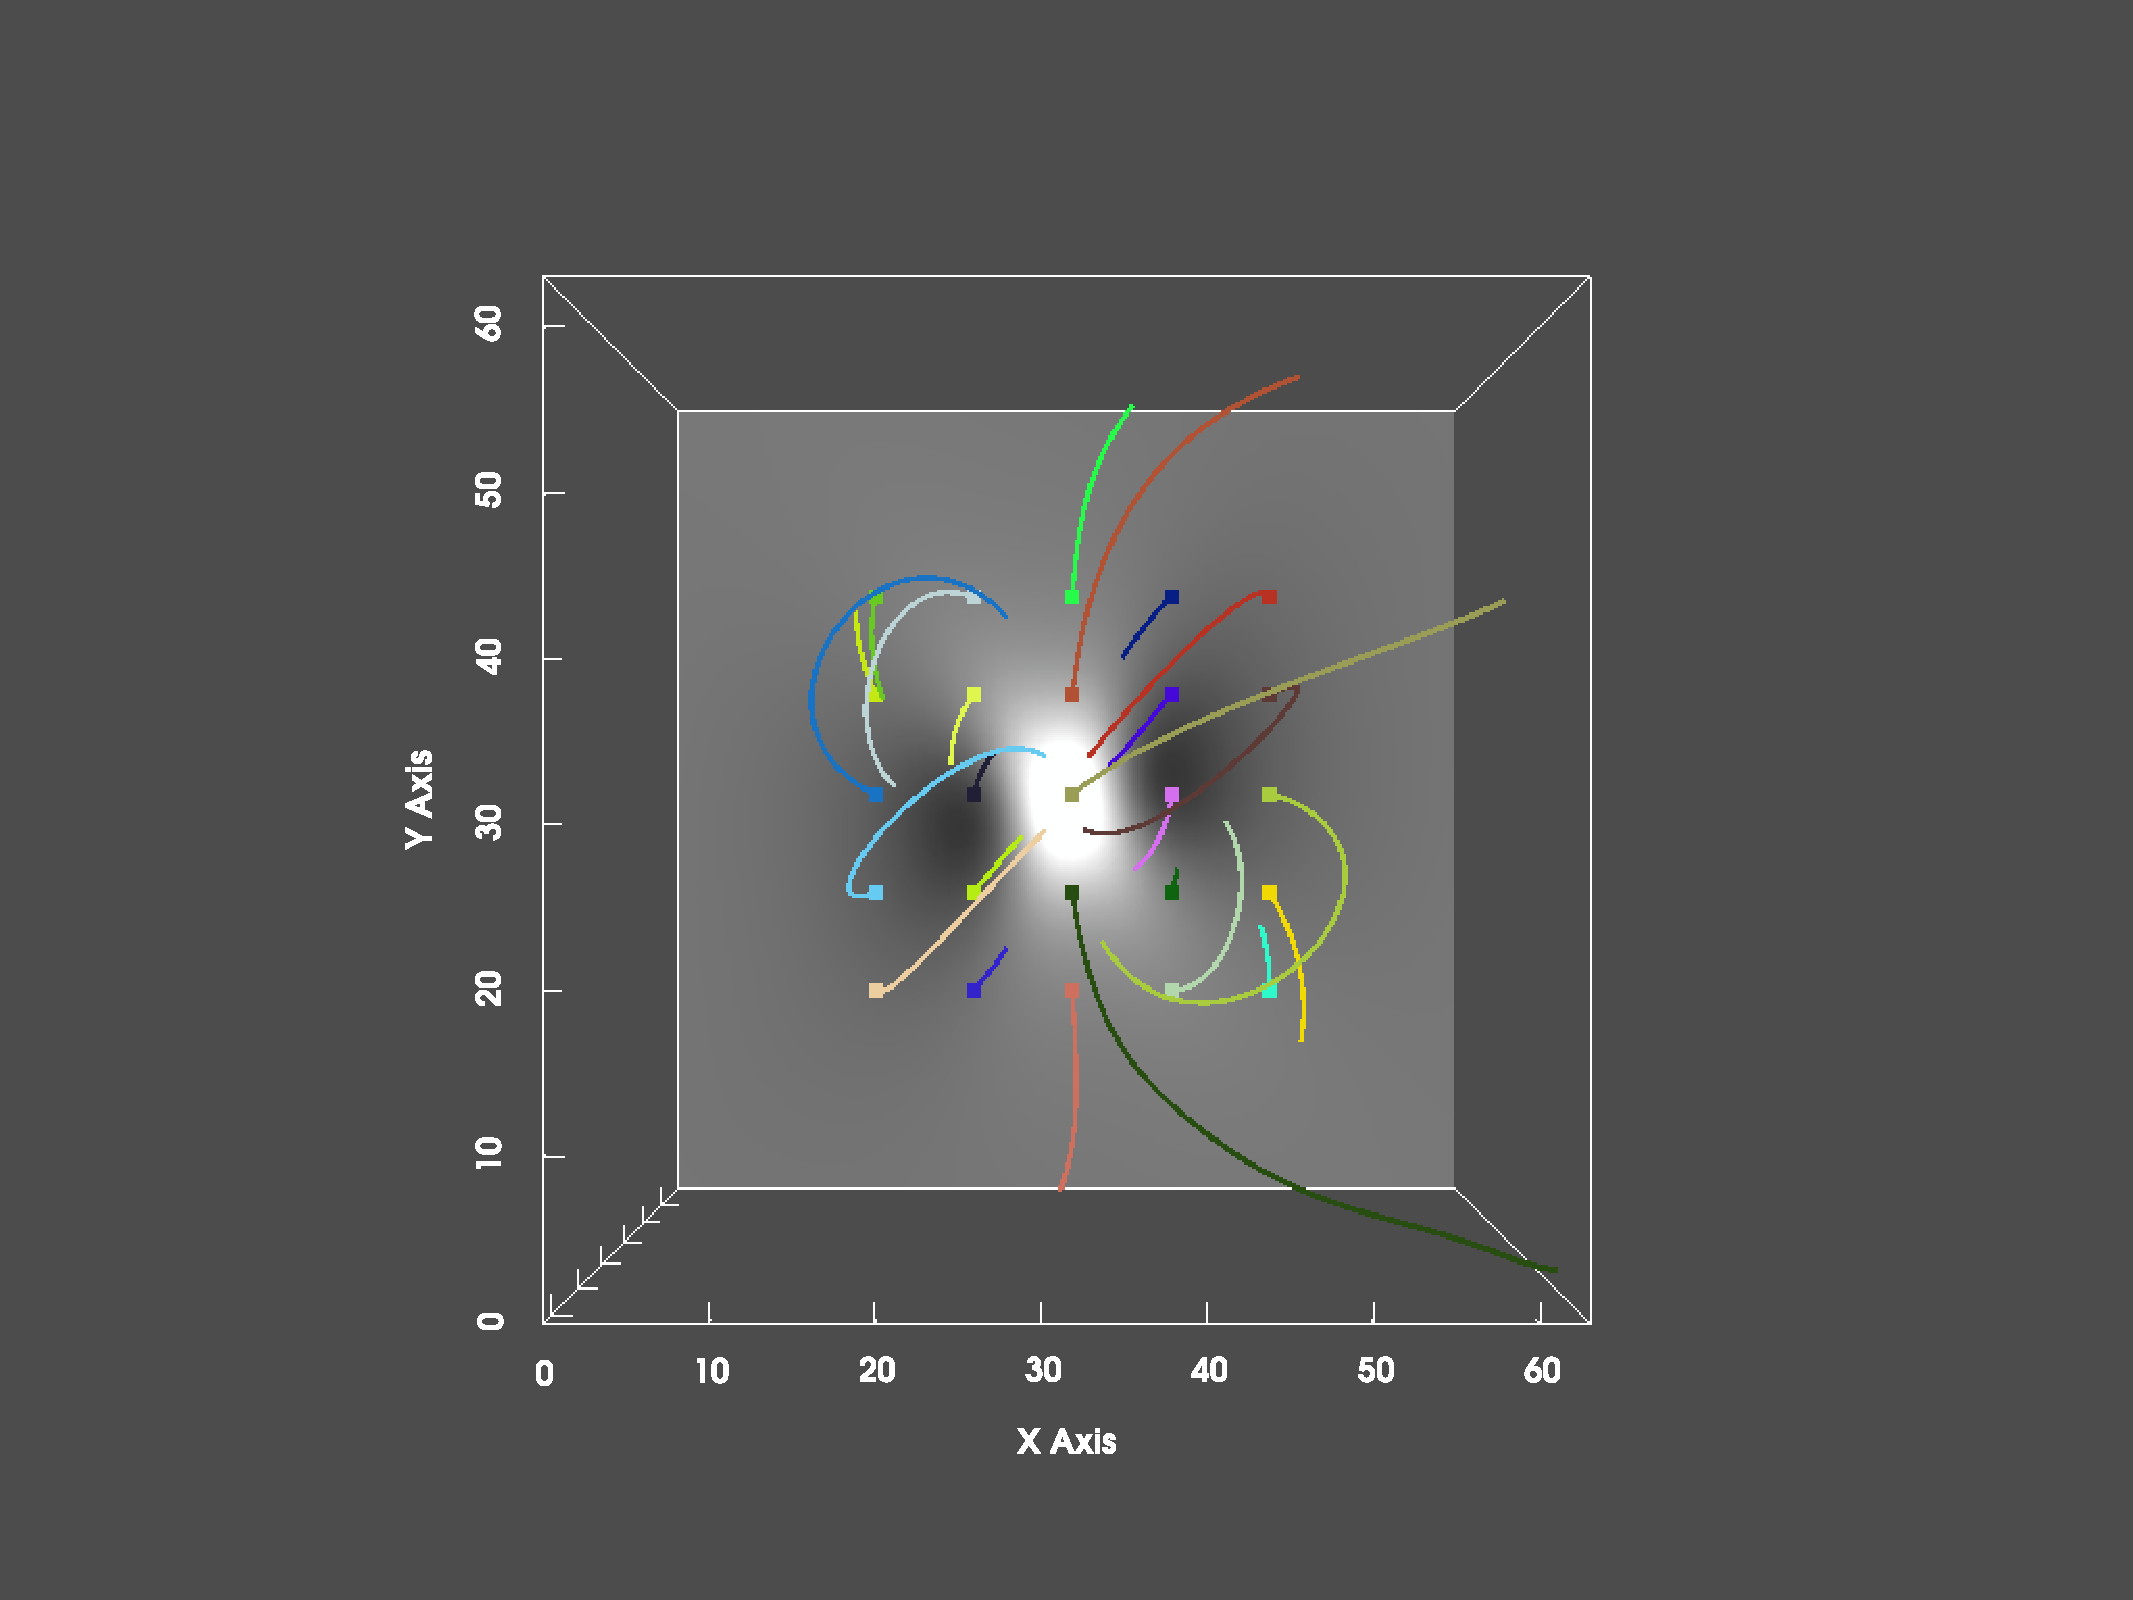
\includegraphics[trim={6cm 1cm 6cm 2cm}, clip, width=\linewidth]{"img/PINN_025000_xy.pdf"}
  \end{subfigure}%
  \begin{subfigure}{.5\linewidth}
    \centering
    \caption{PINN(50000)}
    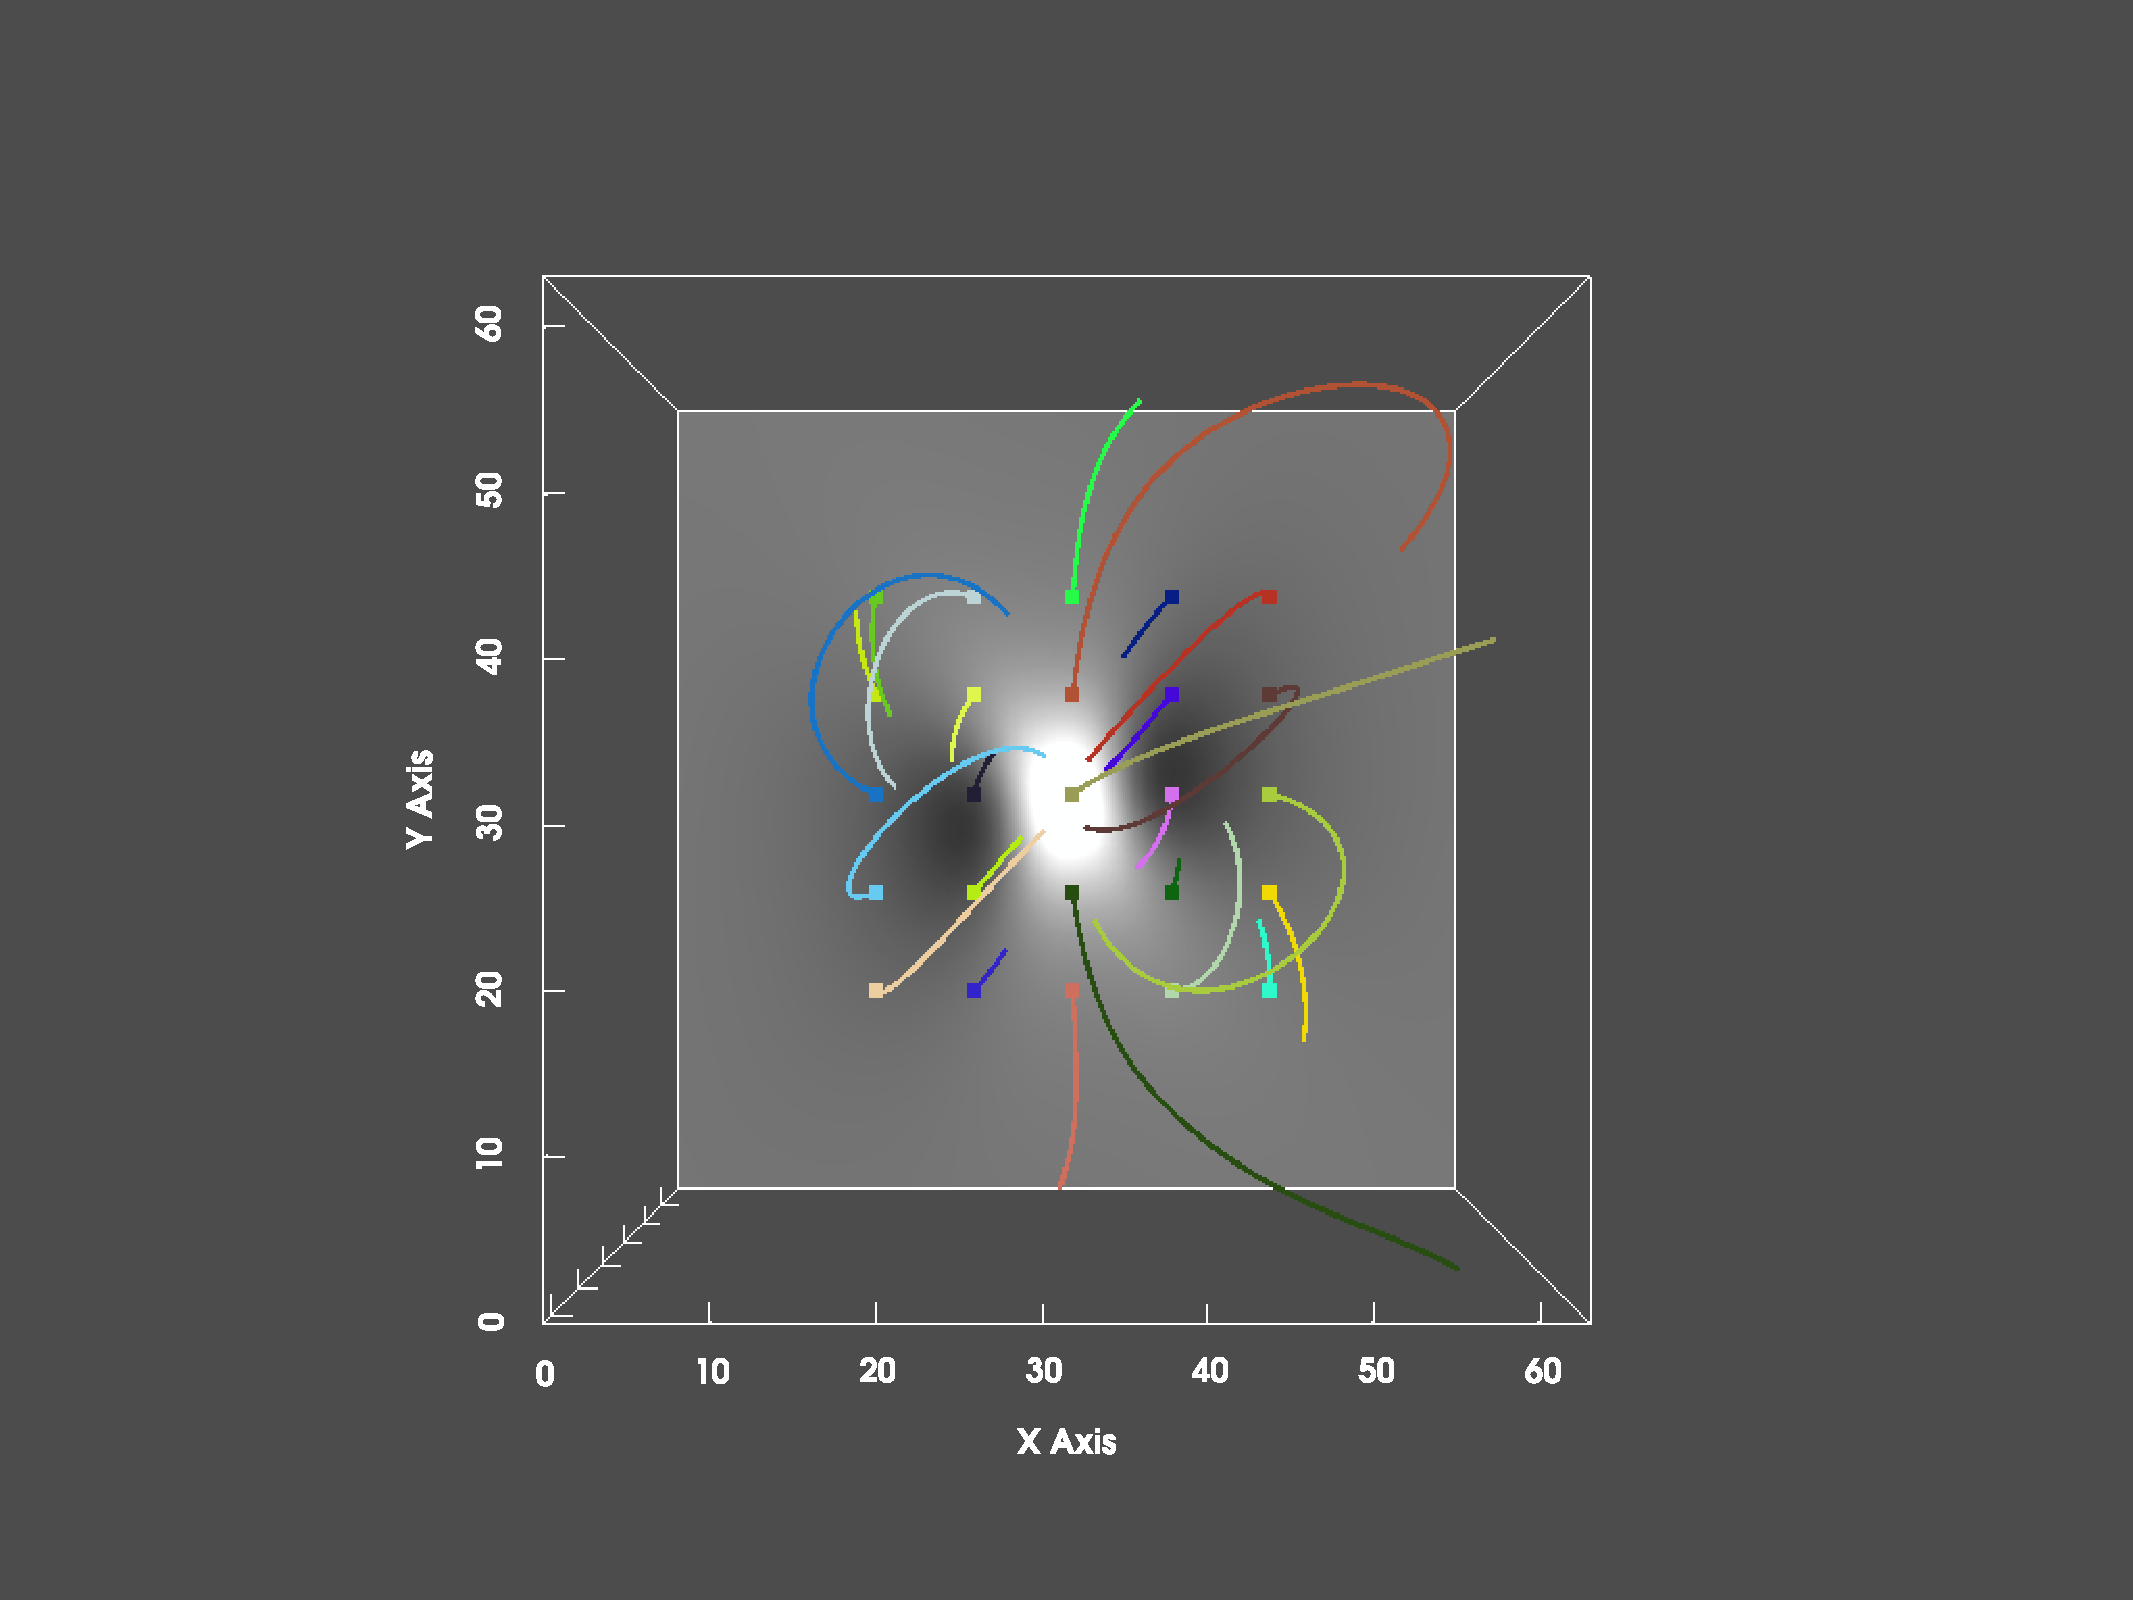
\includegraphics[trim={6cm 1cm 6cm 2cm}, clip, width=\linewidth]{"img/PINN_050000_xy.pdf"}
  \end{subfigure}
  
  \begin{subfigure}{.5\linewidth}
    \centering
    \caption{Potential}
    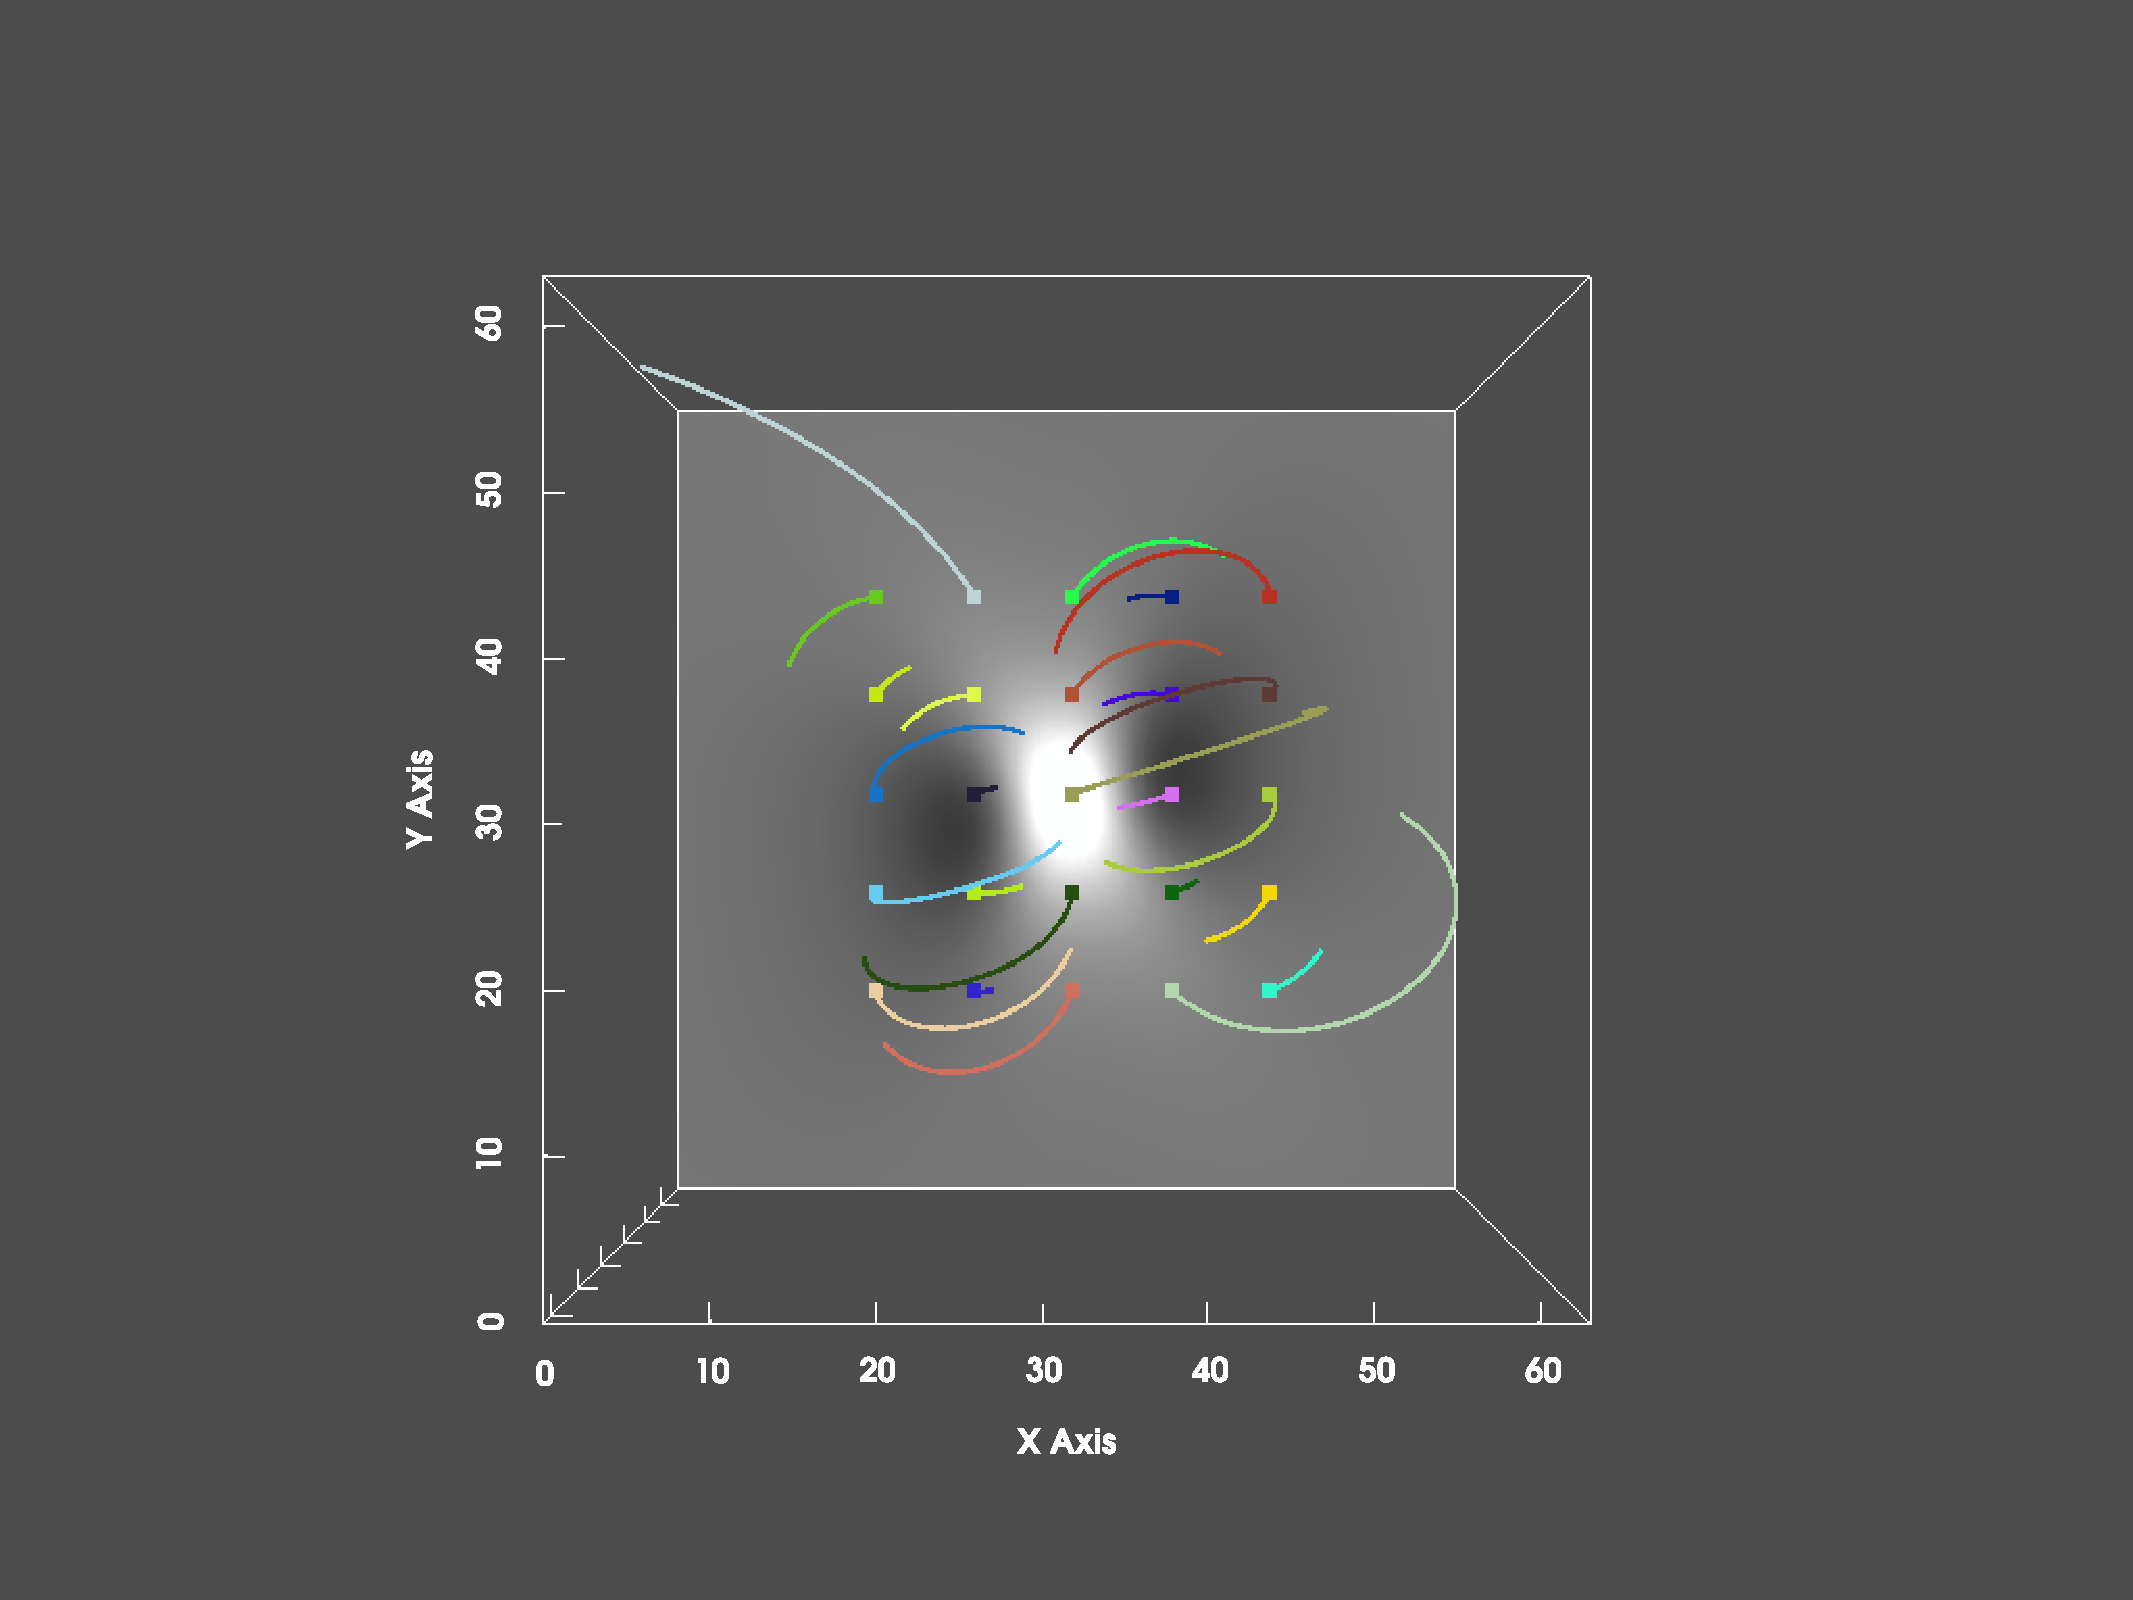
\includegraphics[trim={6cm 1cm 6cm 2cm}, clip, width=\linewidth]{"img/LL_pot_xy.pdf"}
  \end{subfigure}%
  \begin{subfigure}{.5\linewidth}
    \centering
    \caption{Low-Lou}
    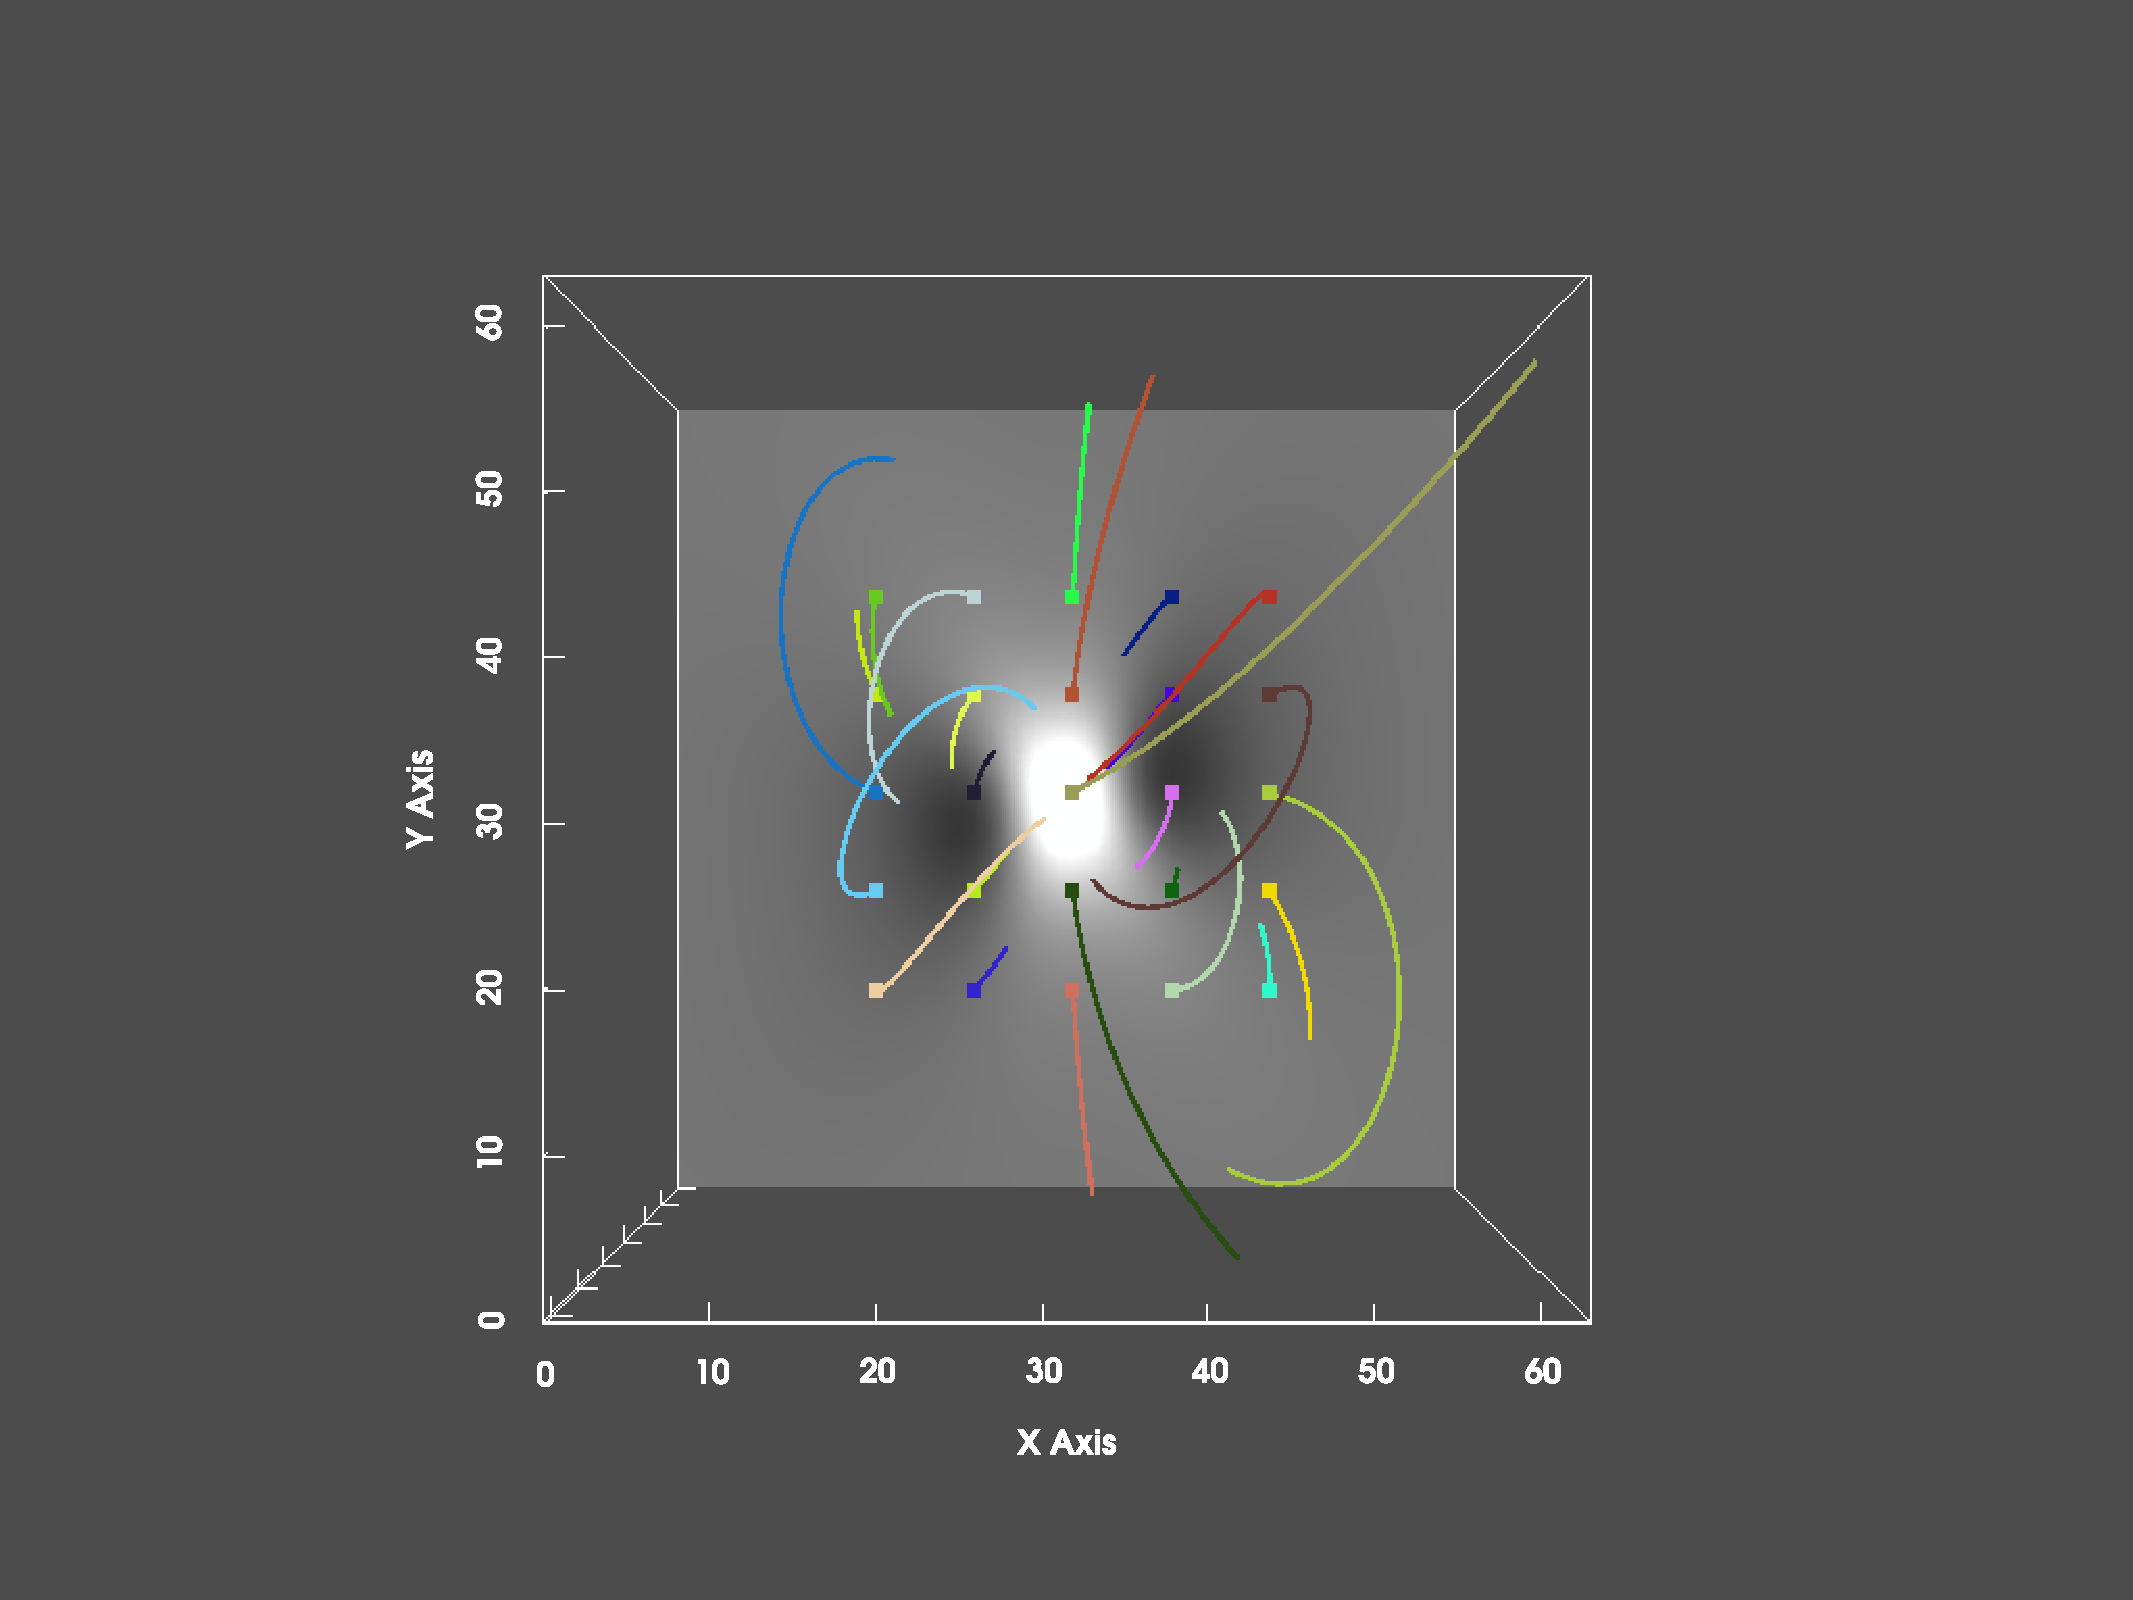
\includegraphics[trim={6cm 1cm 6cm 2cm}, clip, width=\linewidth]{"img/LL_xy.pdf"}
  \end{subfigure}
  
  \caption{The magnetic fields in the xy plane. Each field line is distinguished by its unique color, which is determined by its footpoint at $z=0$ plane.}\label{fig:xy}
\end{figure}

\begin{figure}
  \begin{subfigure}{.5\linewidth}
    \centering
    \caption{PINN(0)}\label{fig:yz0}
    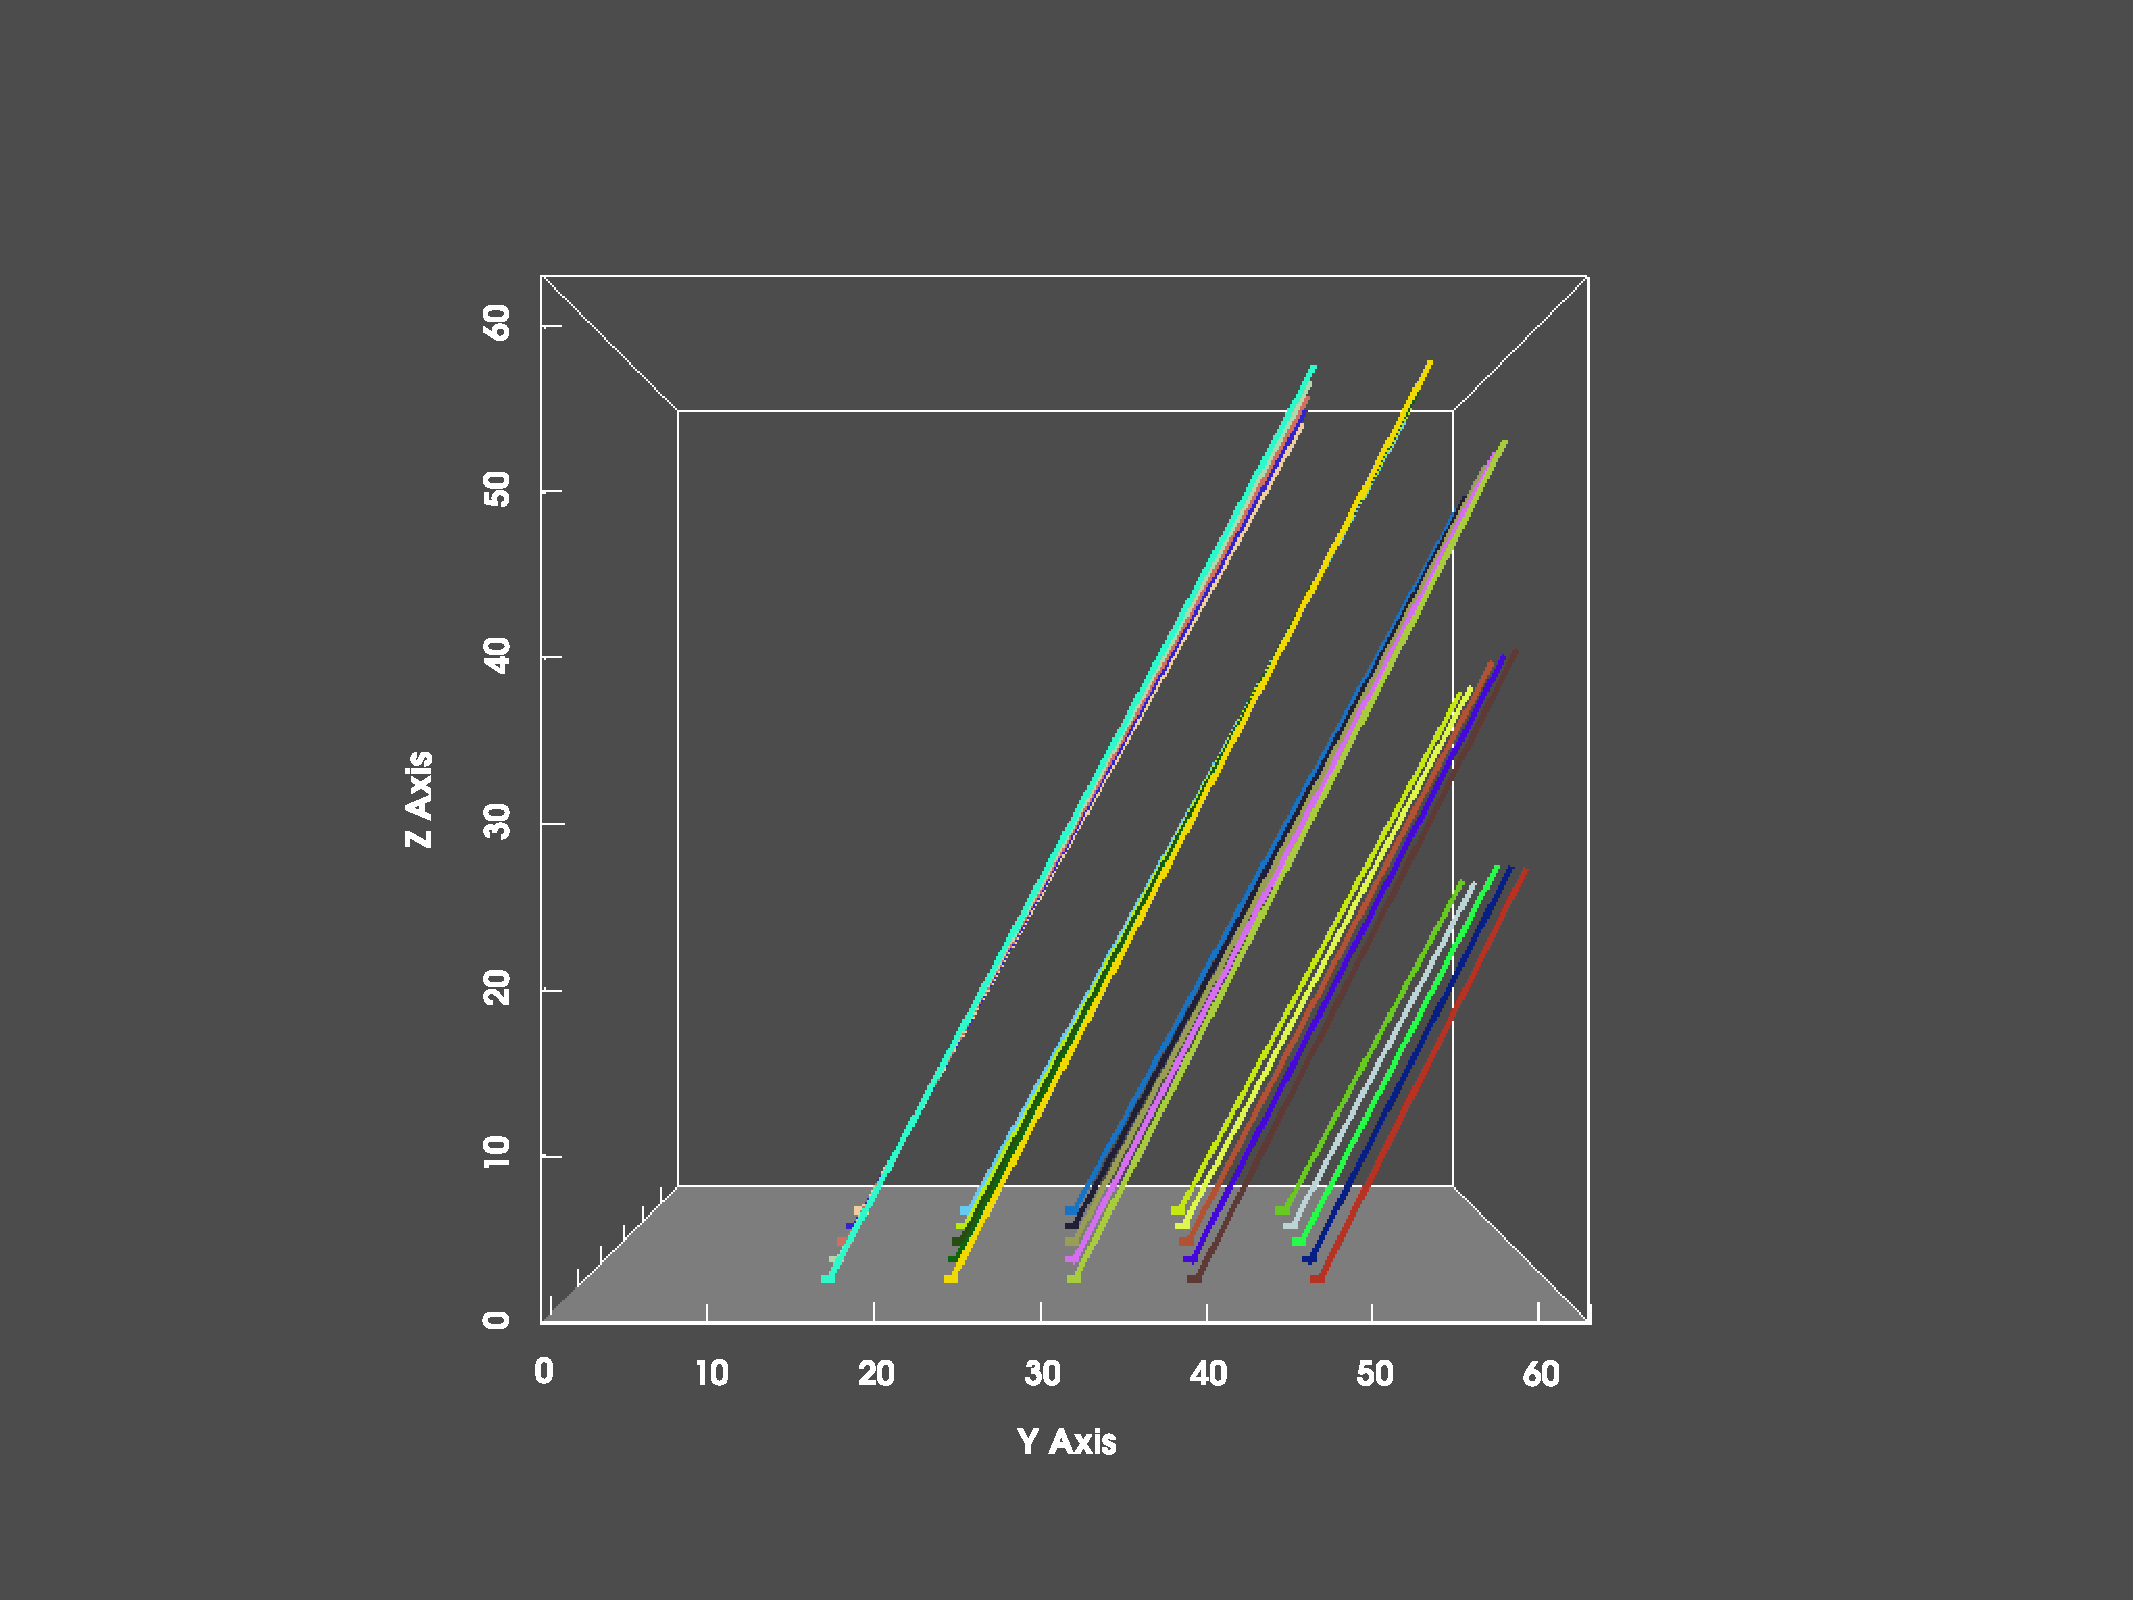
\includegraphics[trim={6cm 1cm 6cm 2cm}, clip, width=\linewidth]{"img/PINN_000000_yz.pdf"}
  \end{subfigure}%
  \begin{subfigure}{.5\linewidth}
    \centering
    \caption{PINN(100)}
    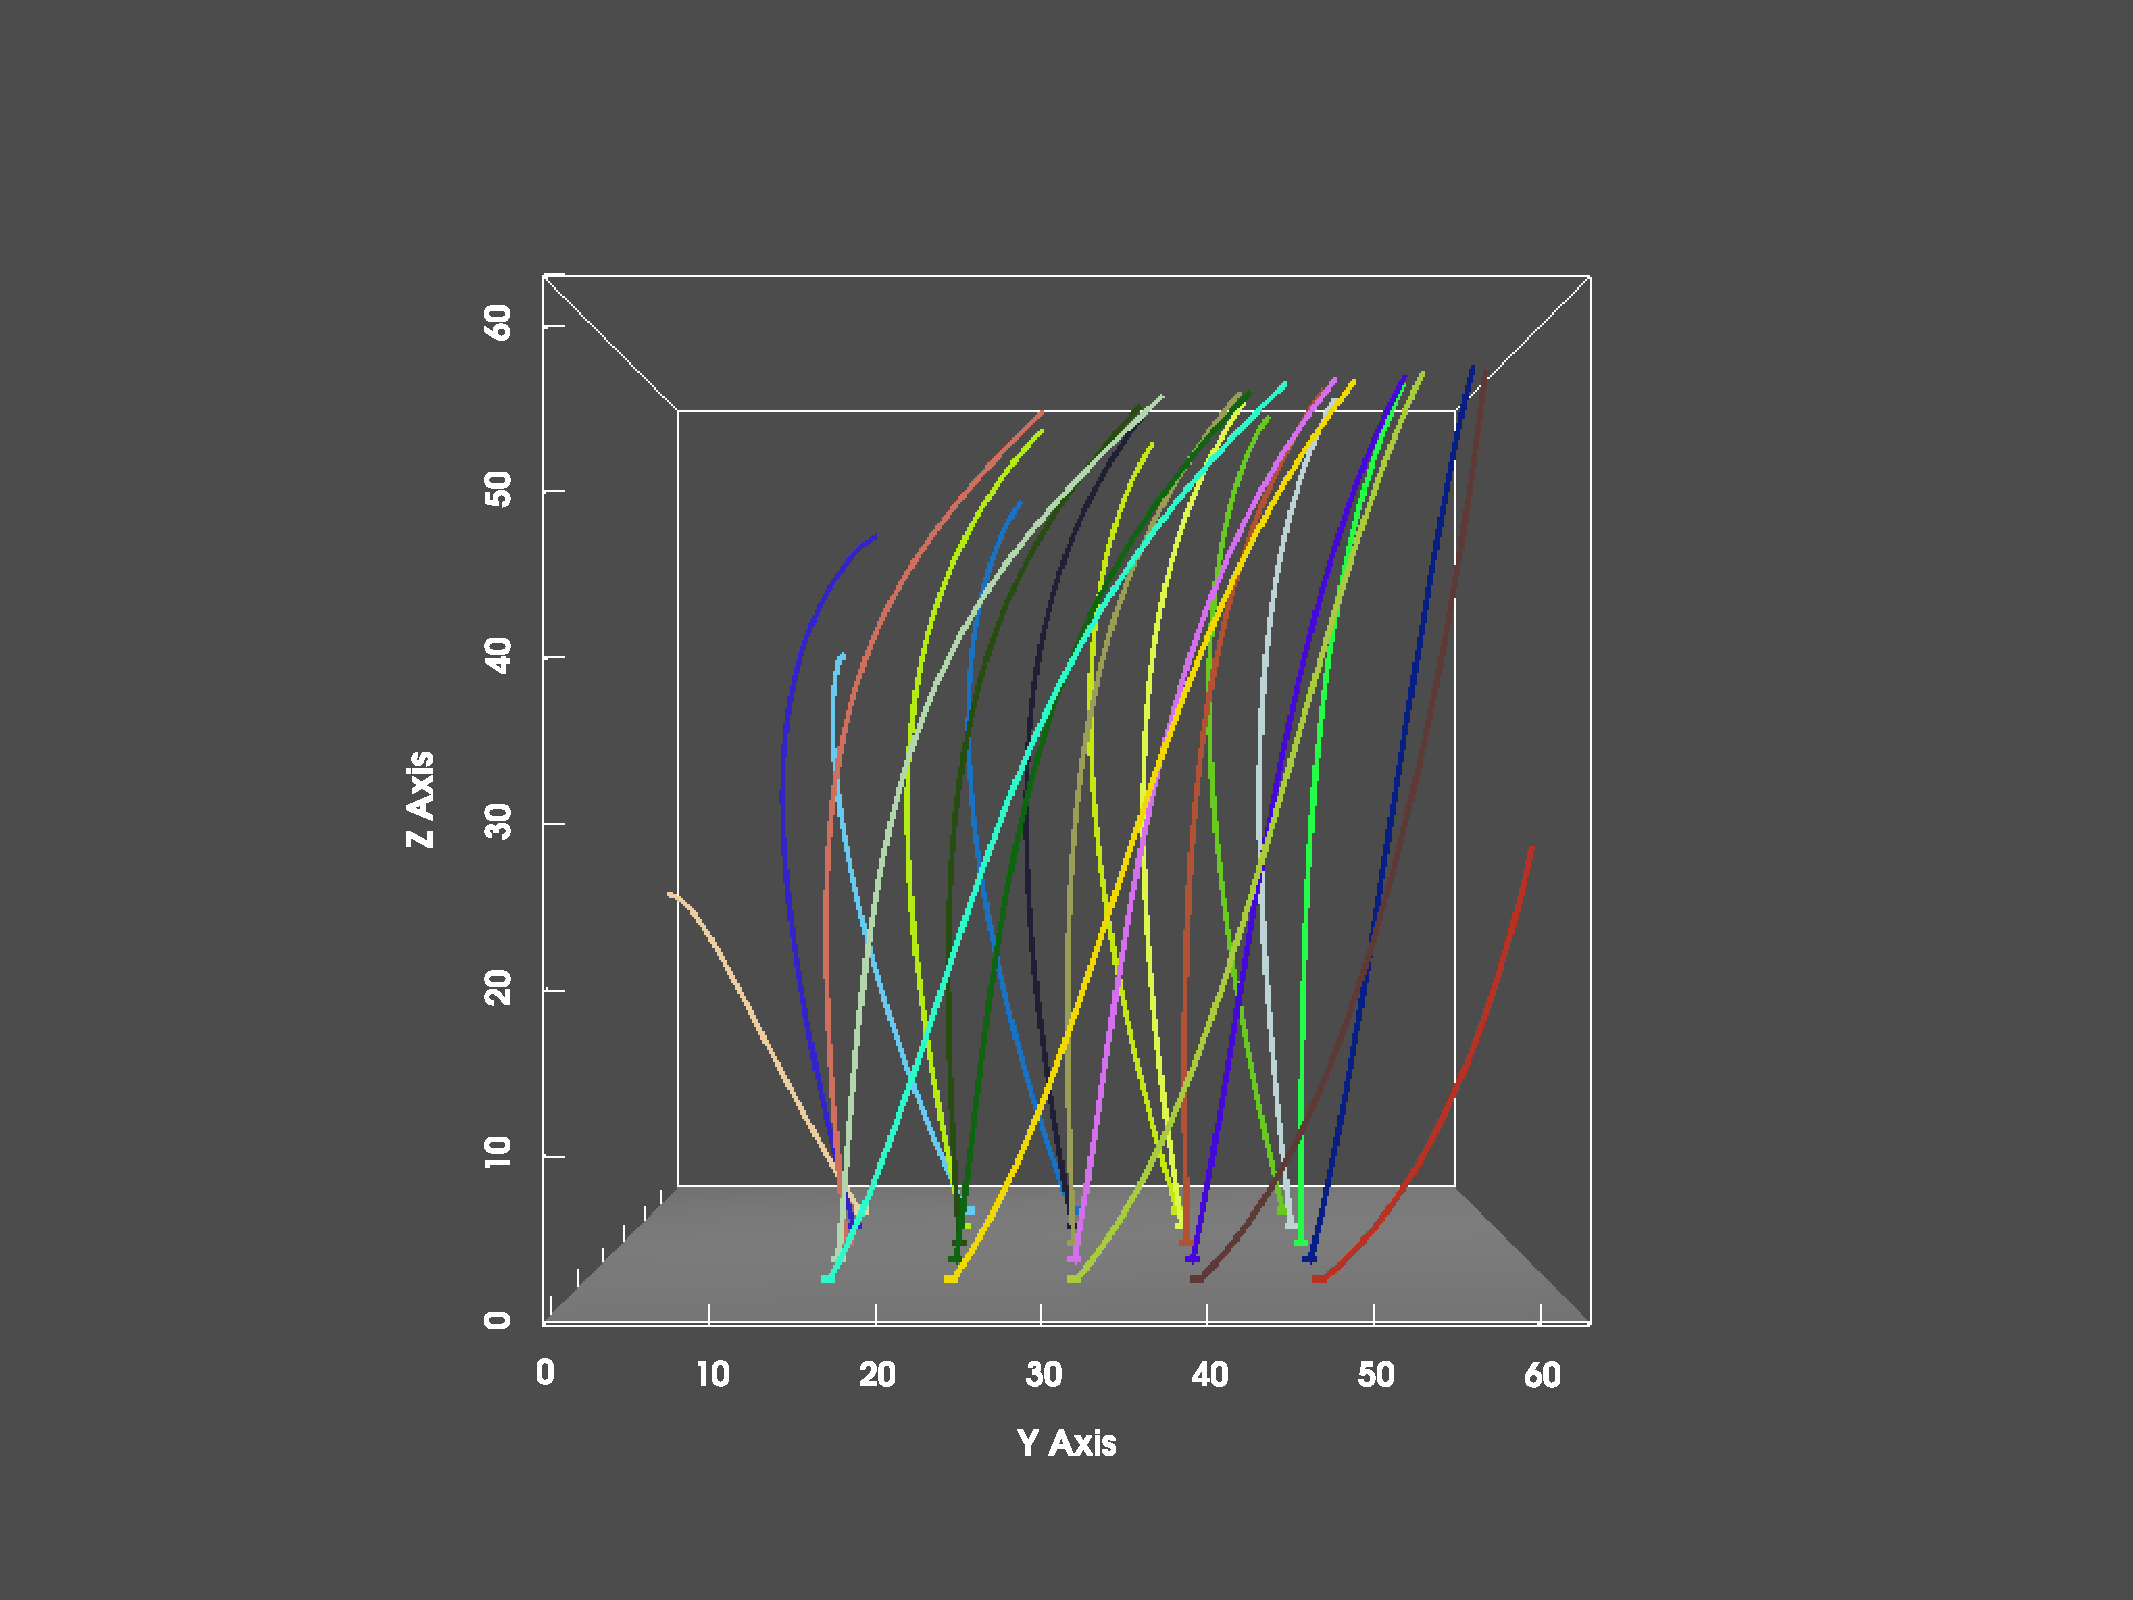
\includegraphics[trim={6cm 1cm 6cm 2cm}, clip, width=\linewidth]{"img/PINN_000100_yz.pdf"}
  \end{subfigure}

  \begin{subfigure}{.5\linewidth}
    \centering
    \caption{PINN(1000)}
    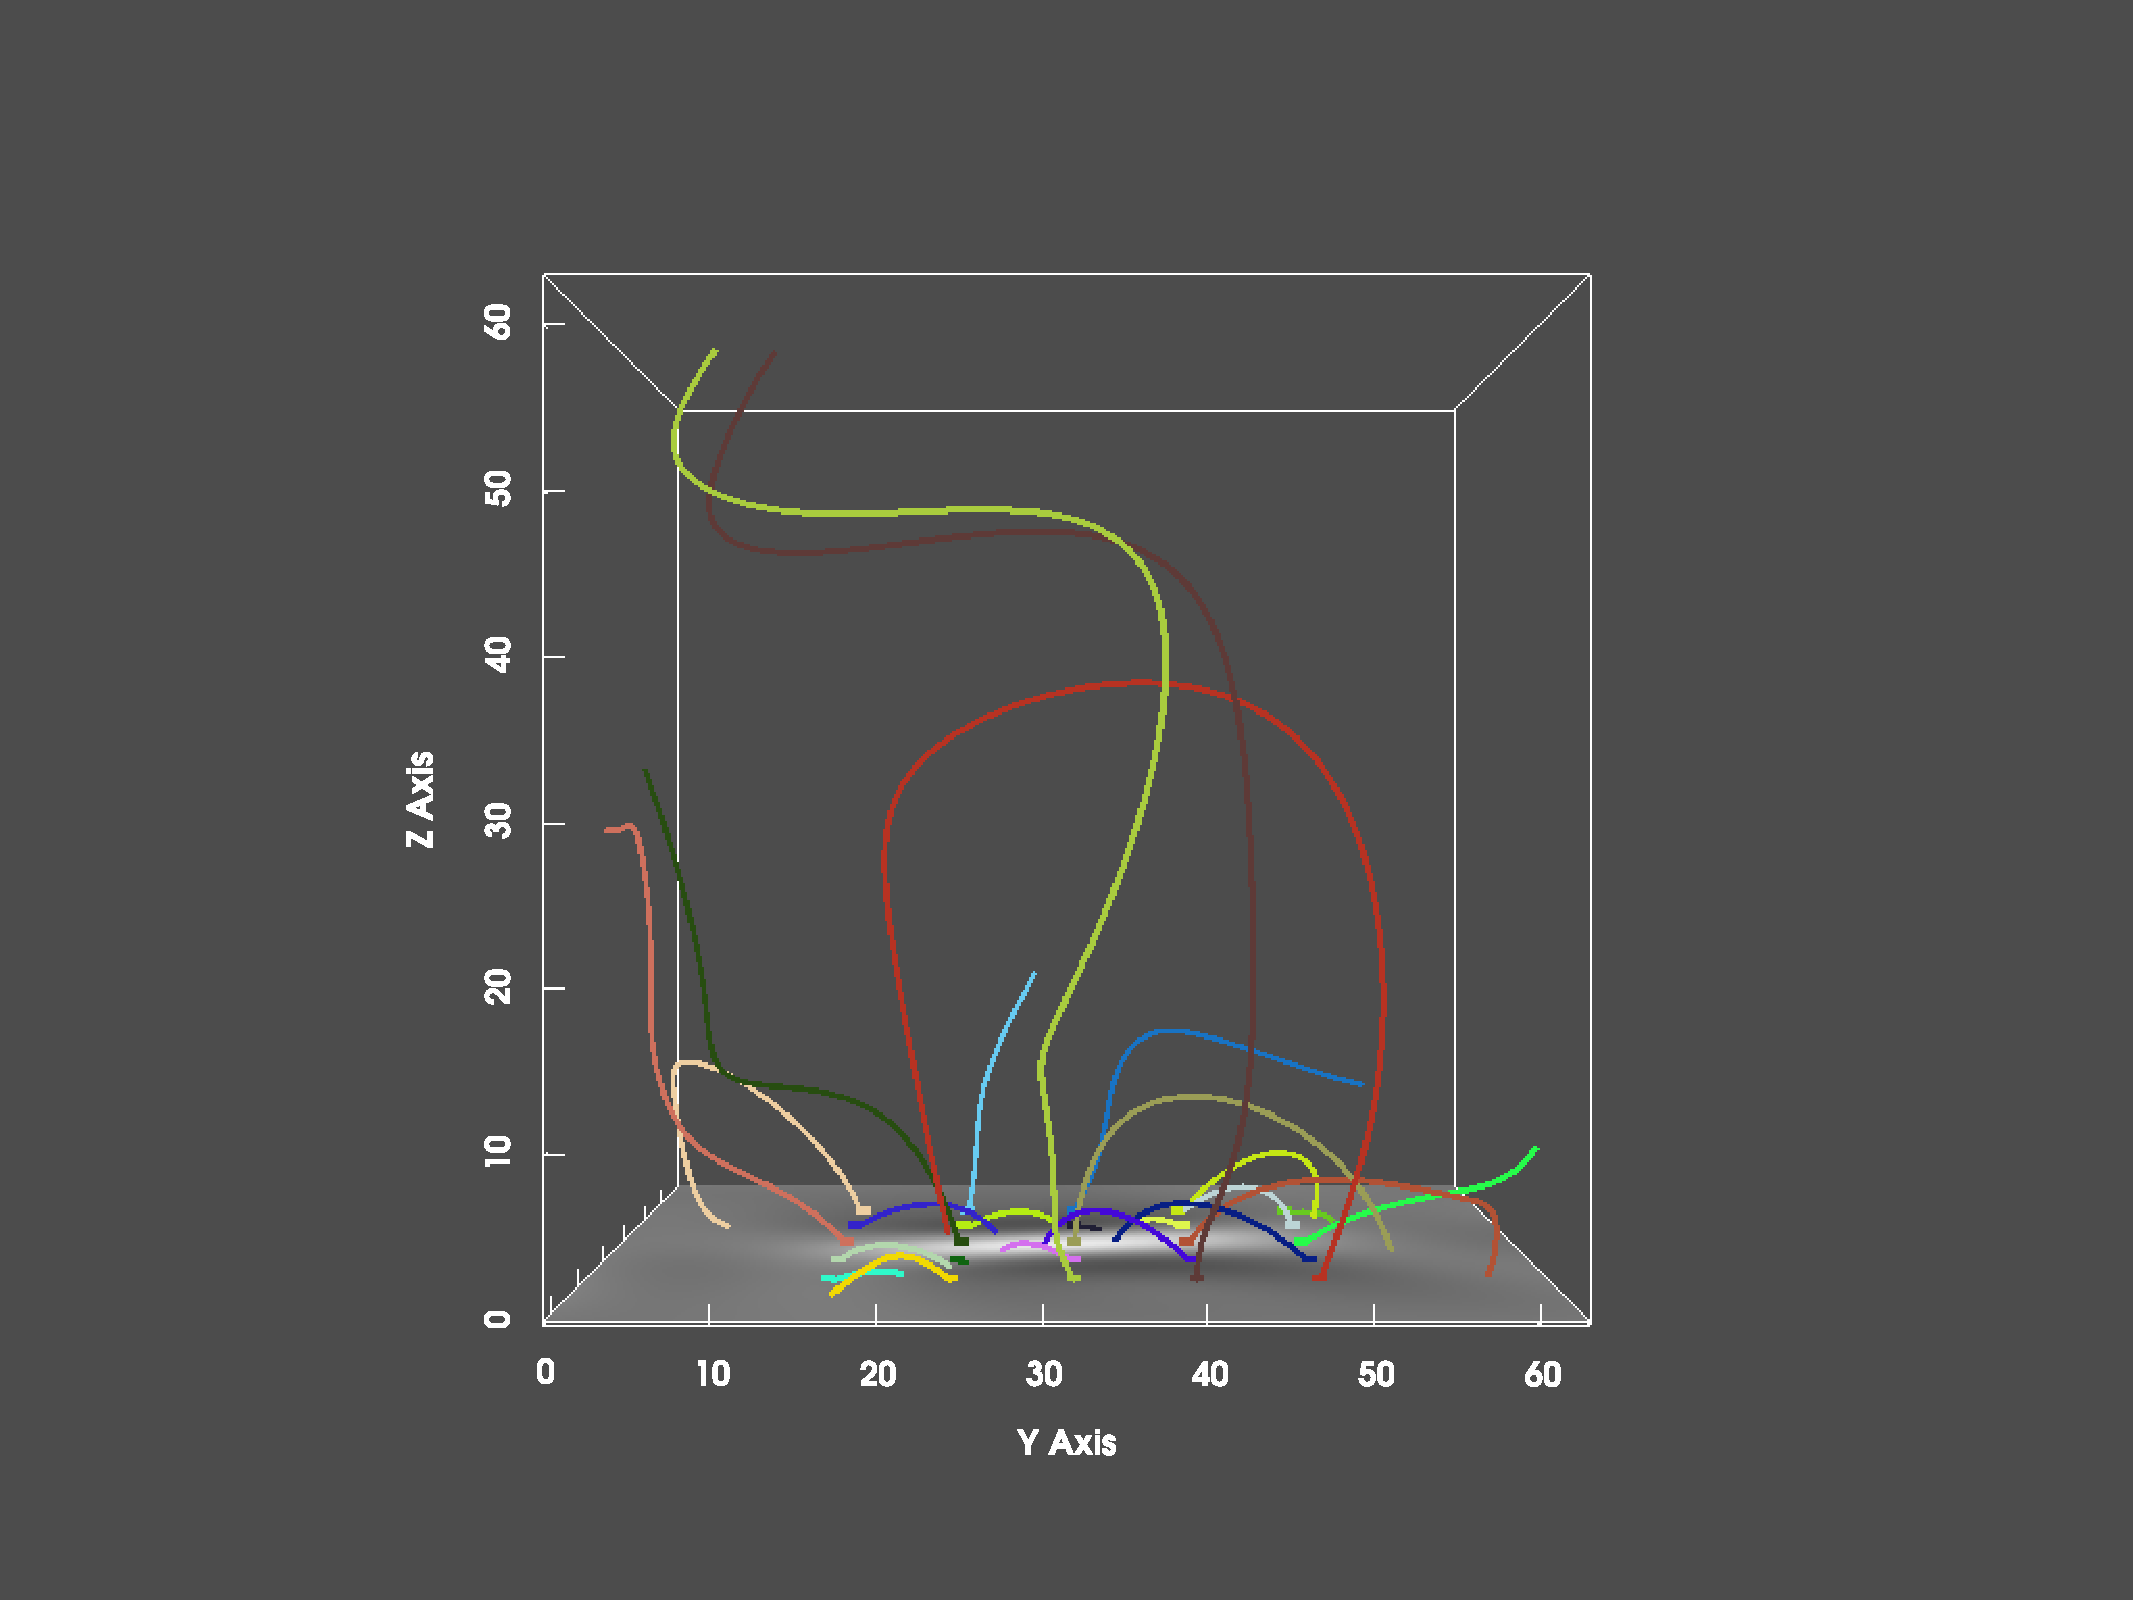
\includegraphics[trim={6cm 1cm 6cm 2cm}, clip, width=\linewidth]{"img/PINN_001000_yz.pdf"}
  \end{subfigure}%
  \begin{subfigure}{.5\linewidth}
    \centering
    \caption{PINN(10000)}
    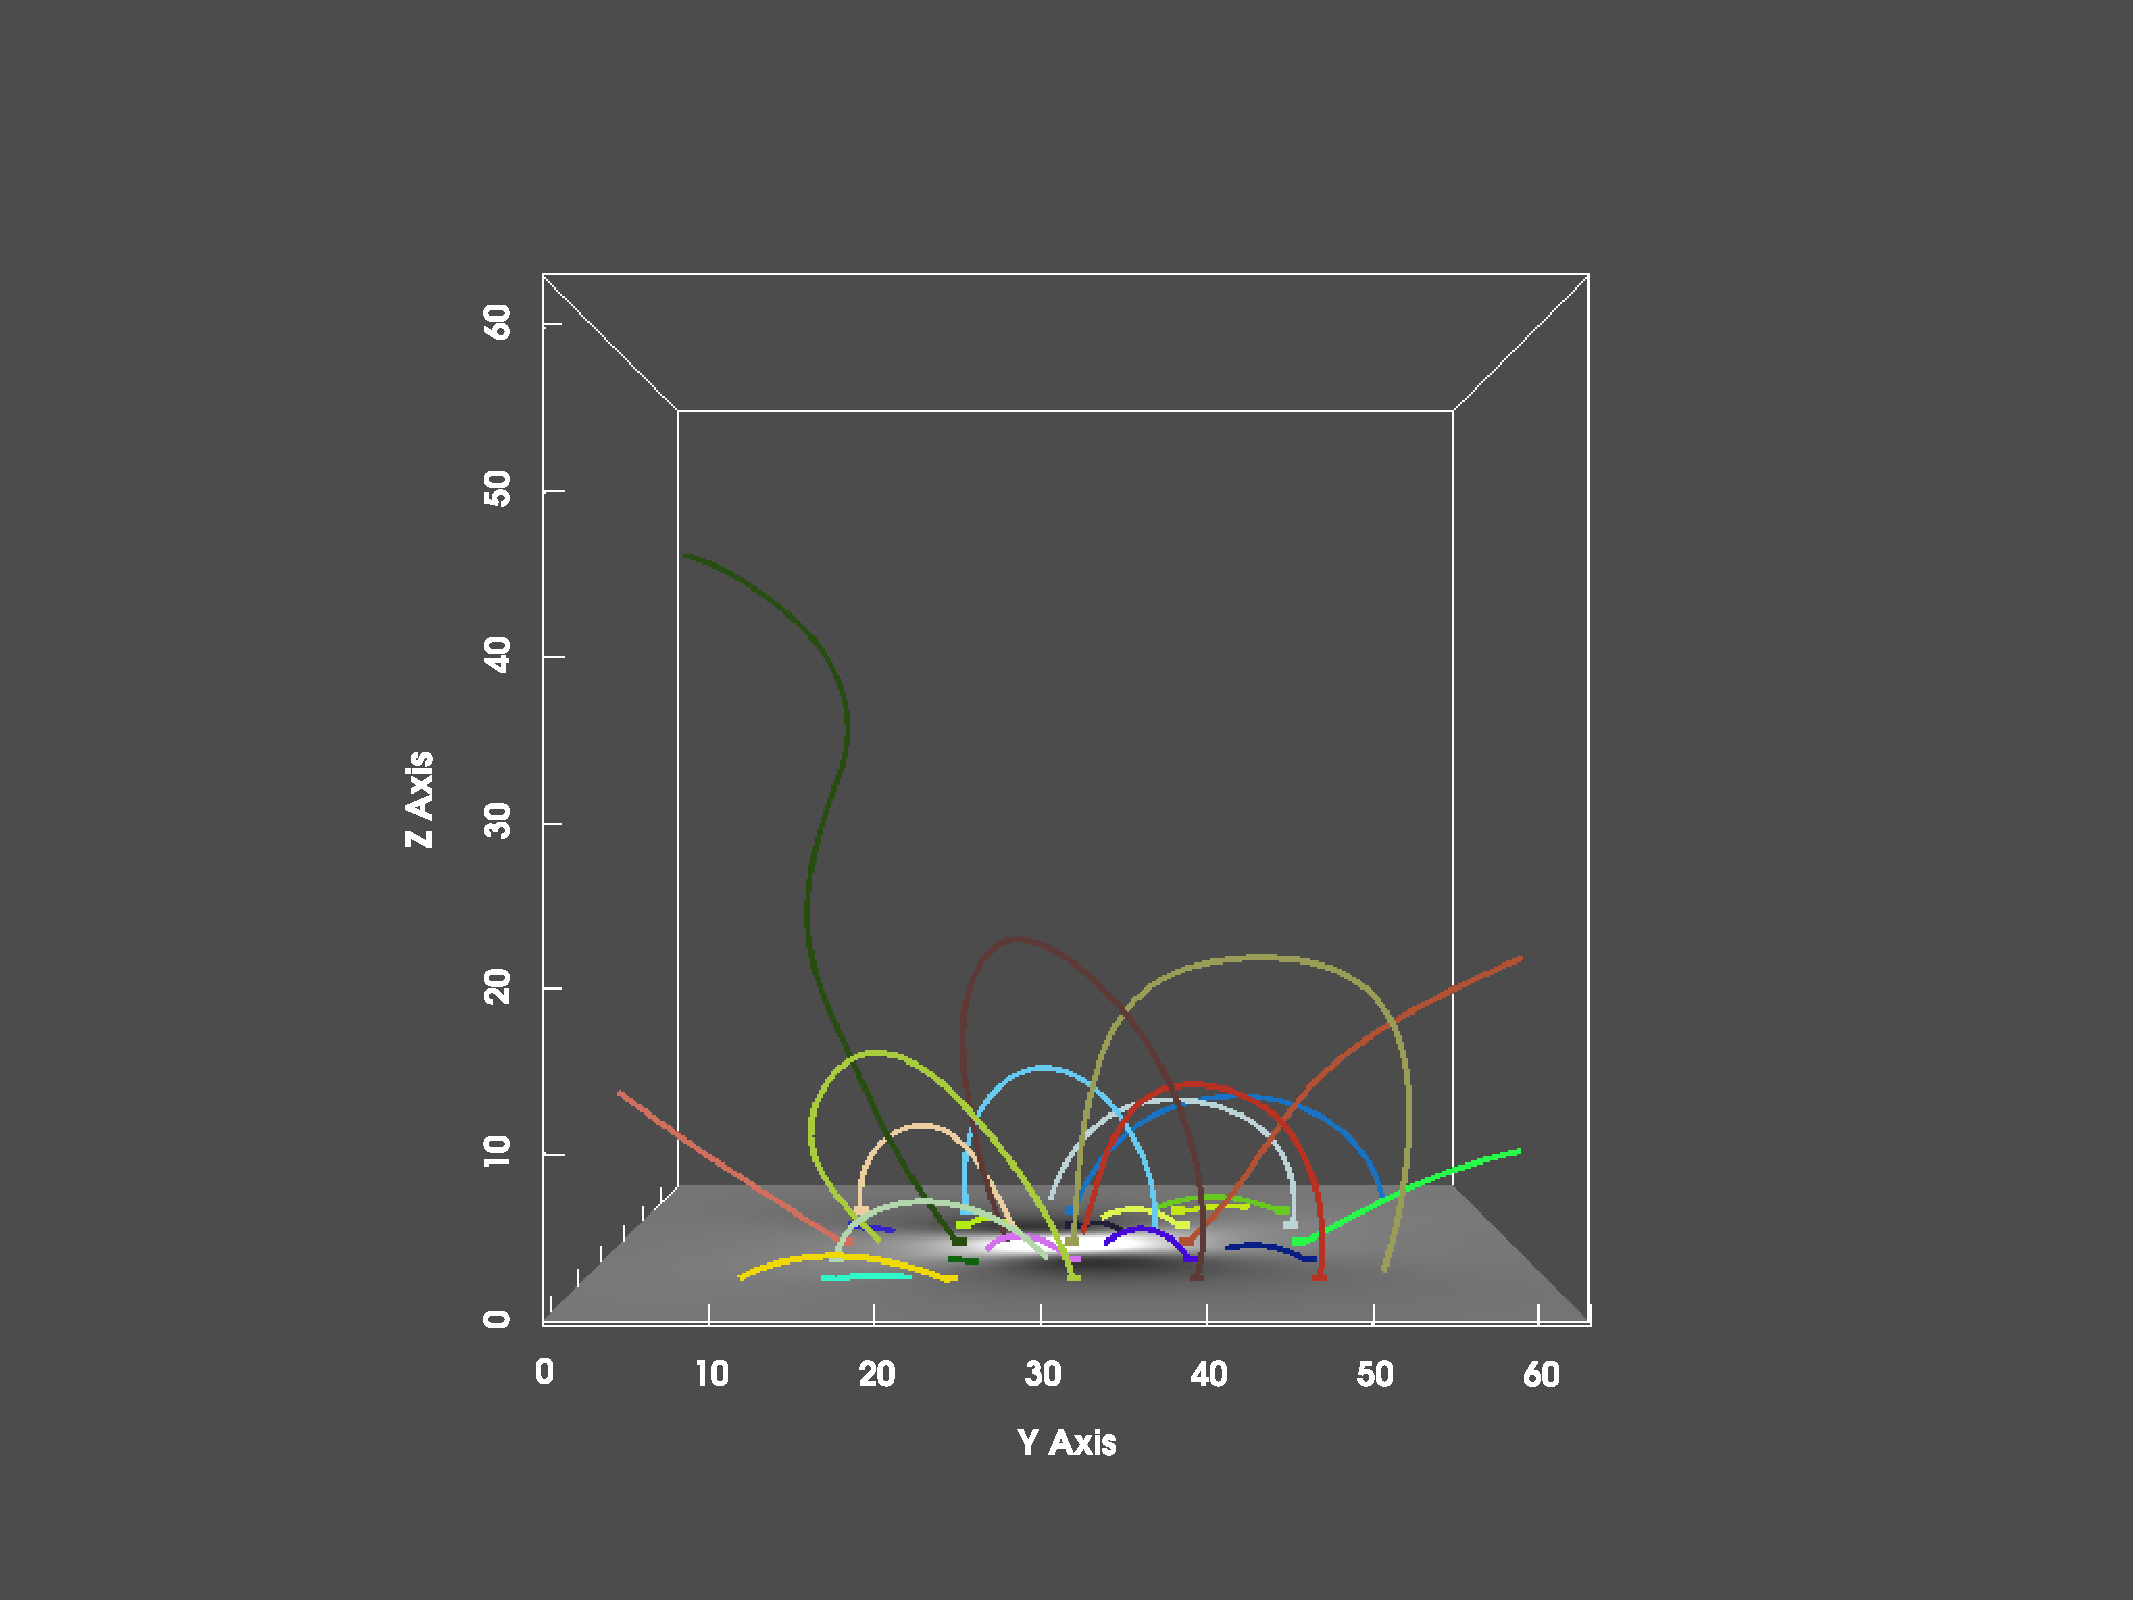
\includegraphics[trim={6cm 1cm 6cm 2cm}, clip, width=\linewidth]{"img/PINN_010000_yz.pdf"}
  \end{subfigure}

  \begin{subfigure}{.5\linewidth}
    \centering
    \caption{PINN(25000)}
    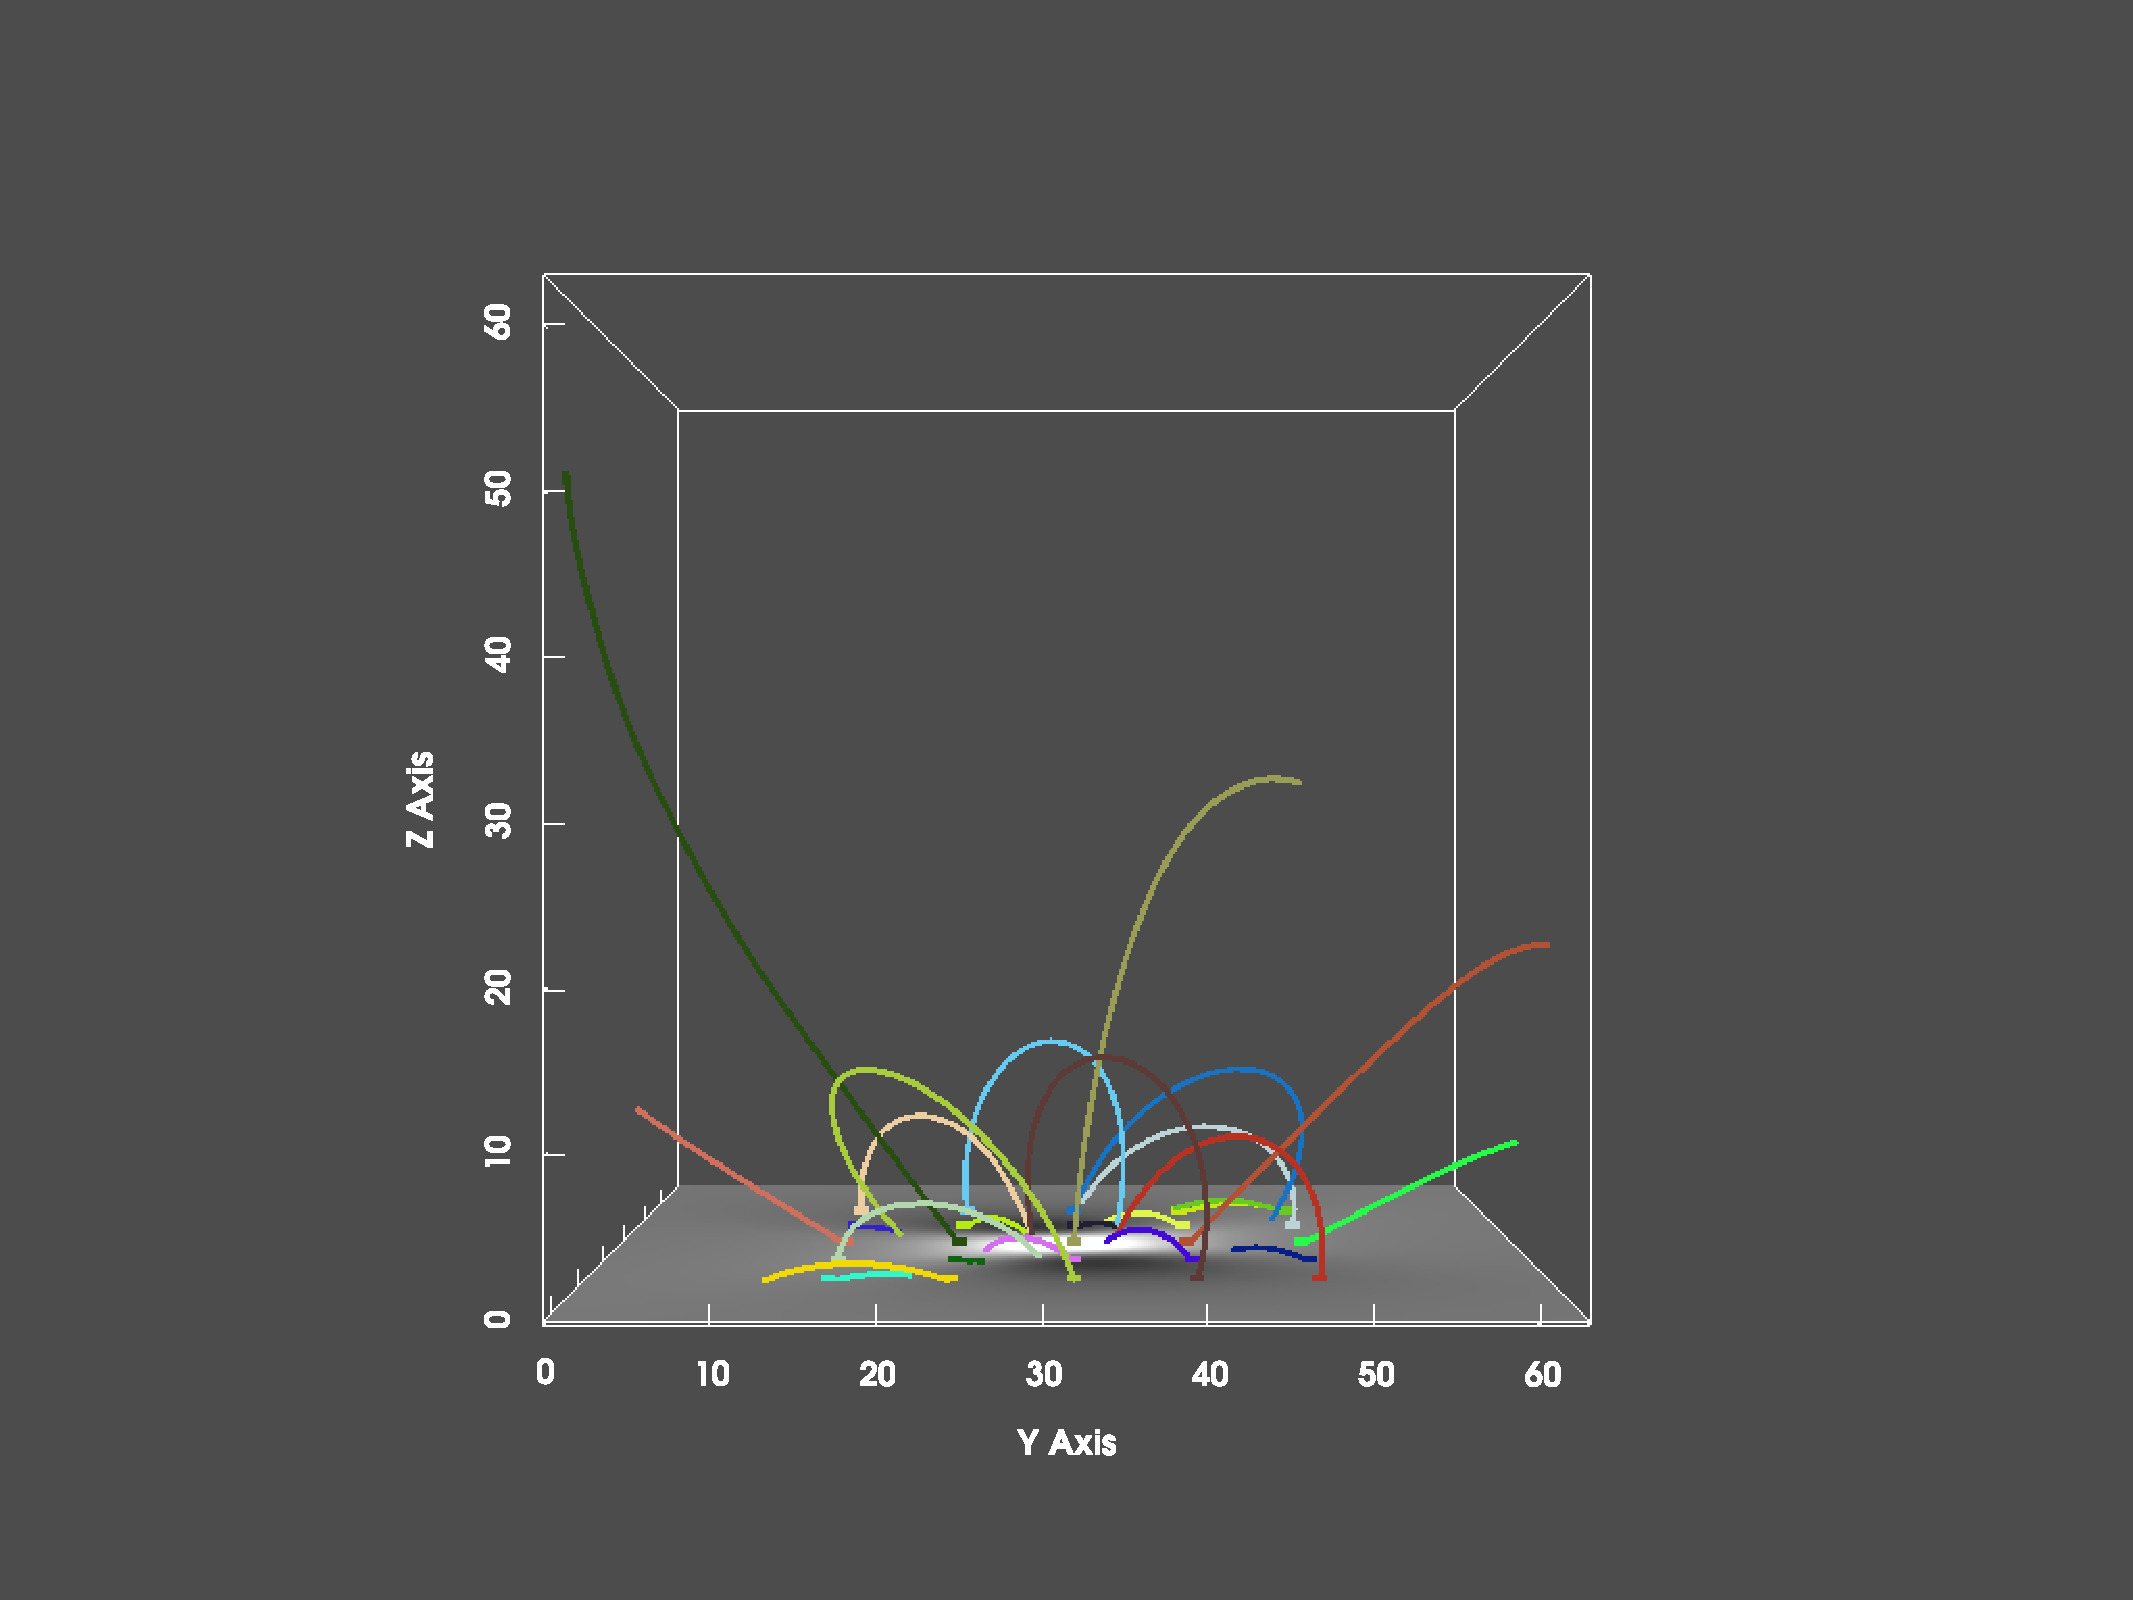
\includegraphics[trim={6cm 1cm 6cm 2cm}, clip, width=\linewidth]{"img/PINN_025000_yz.pdf"}
  \end{subfigure}%
  \begin{subfigure}{.5\linewidth}
    \centering
    \caption{PINN(50000)}
    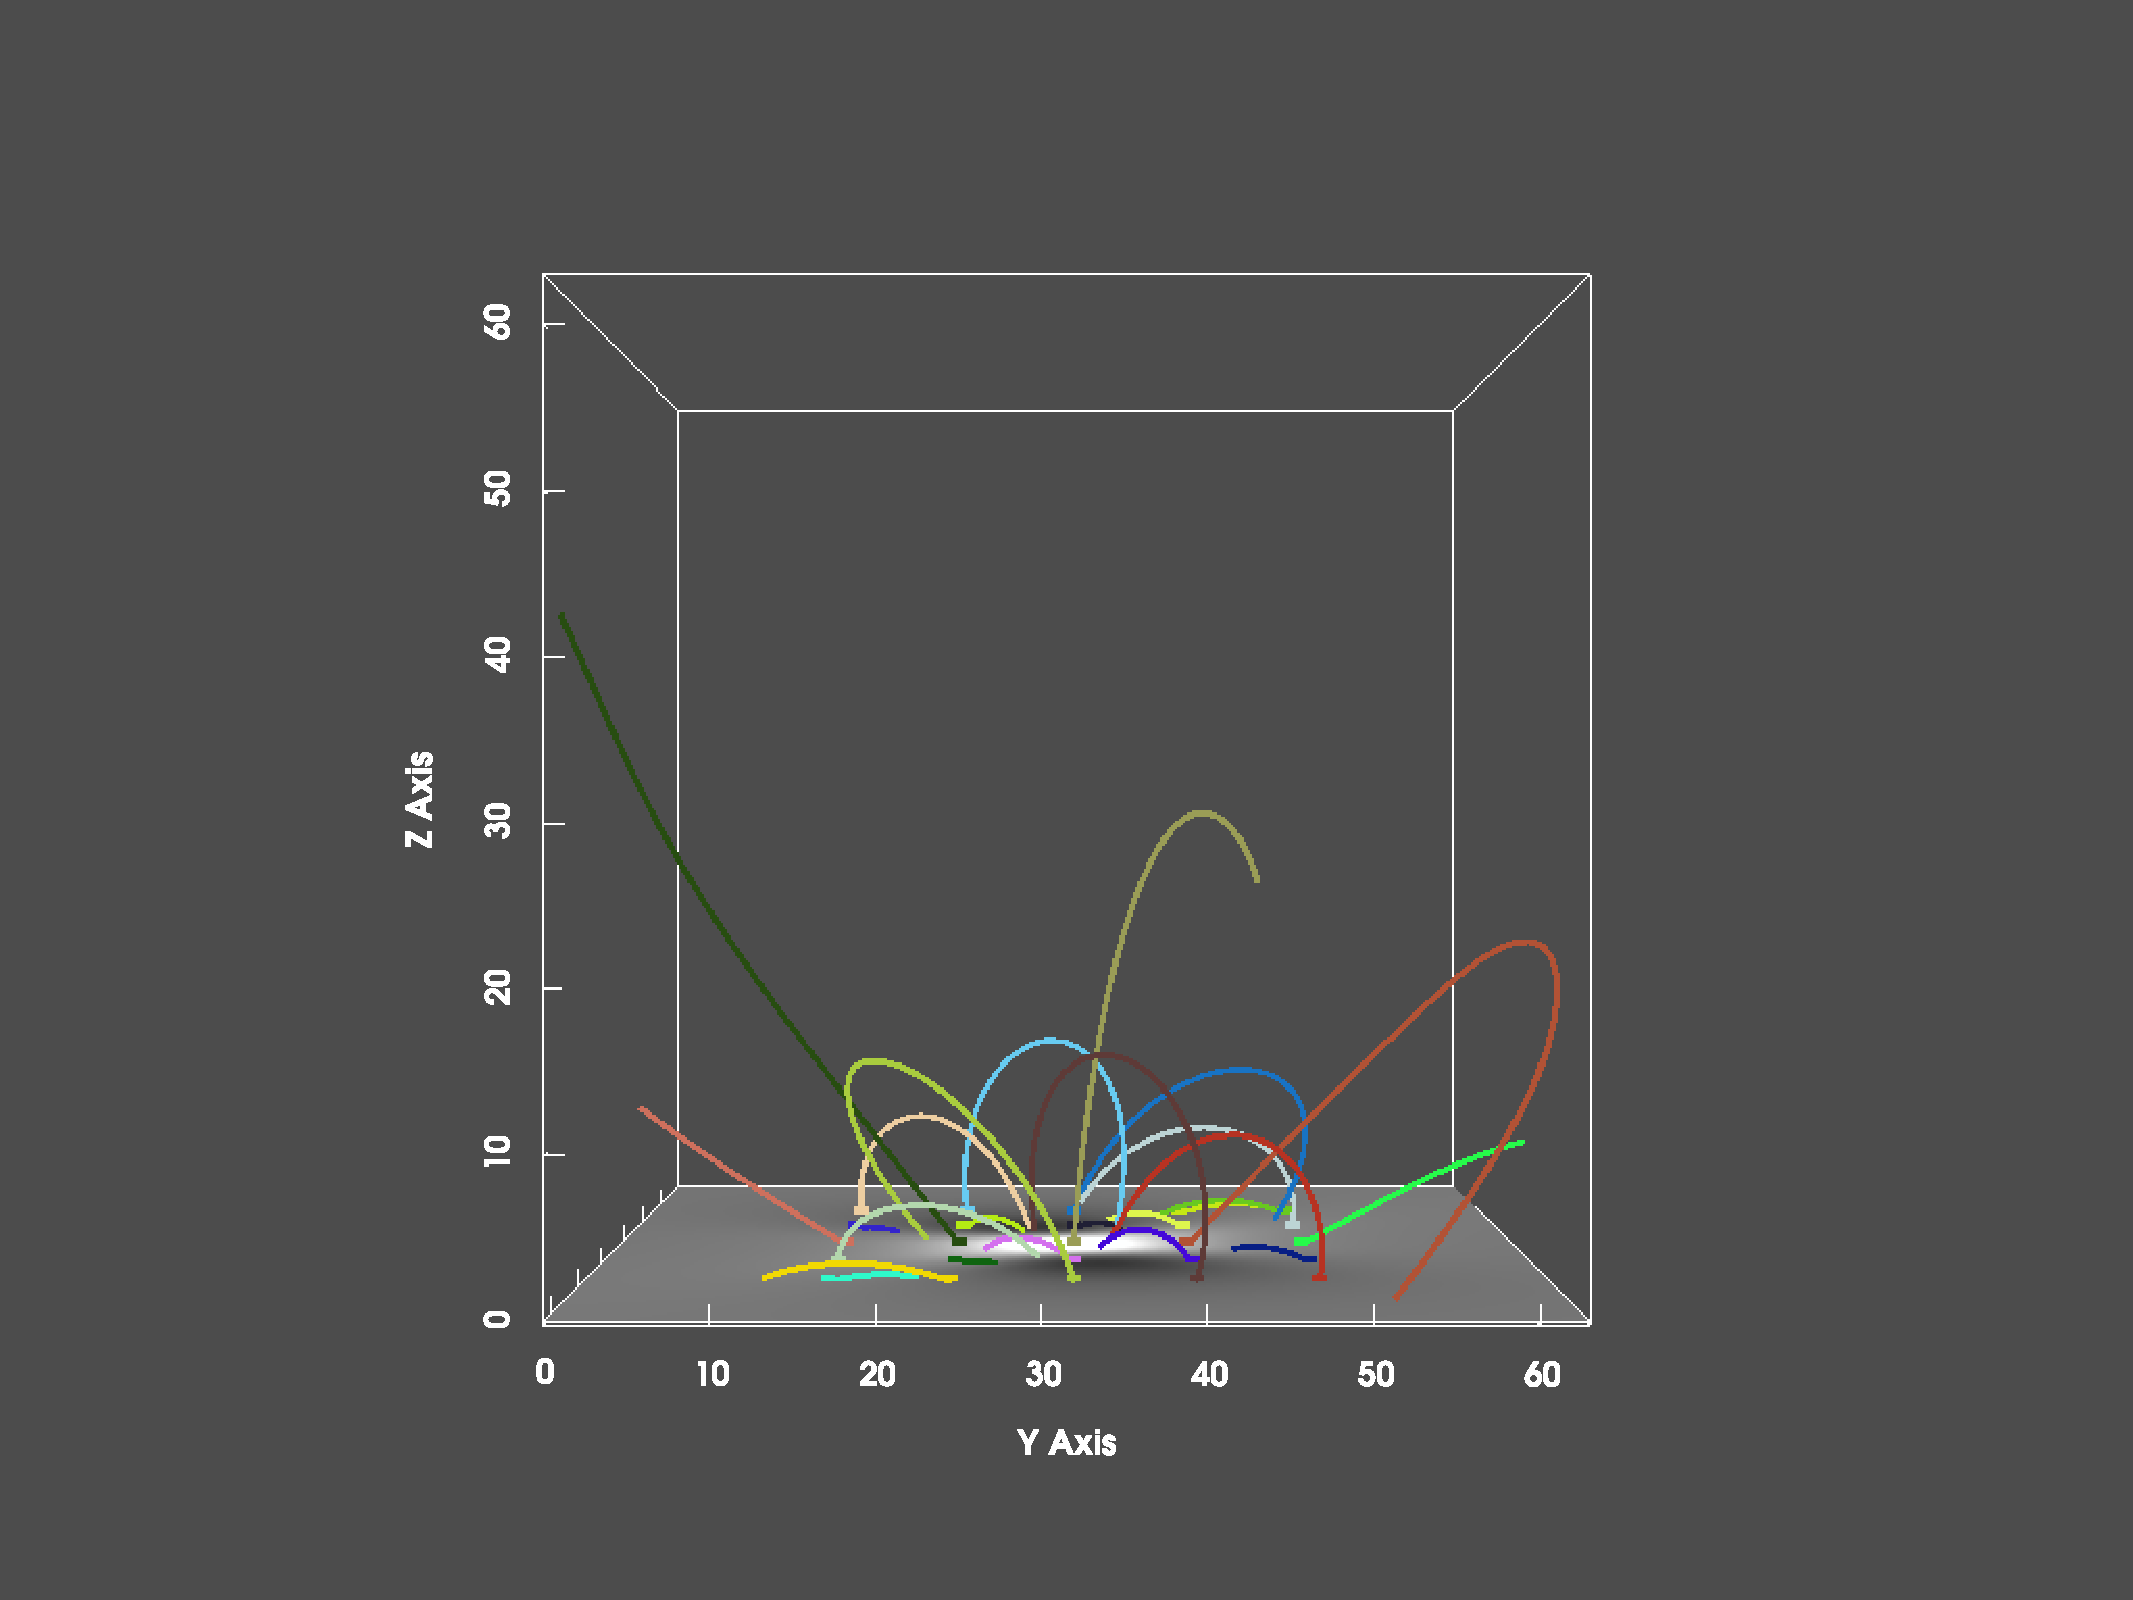
\includegraphics[trim={6cm 1cm 6cm 2cm}, clip, width=\linewidth]{"img/PINN_050000_yz.pdf"}
  \end{subfigure}
  
  \begin{subfigure}{.5\linewidth}
    \centering
    \caption{Potential}
    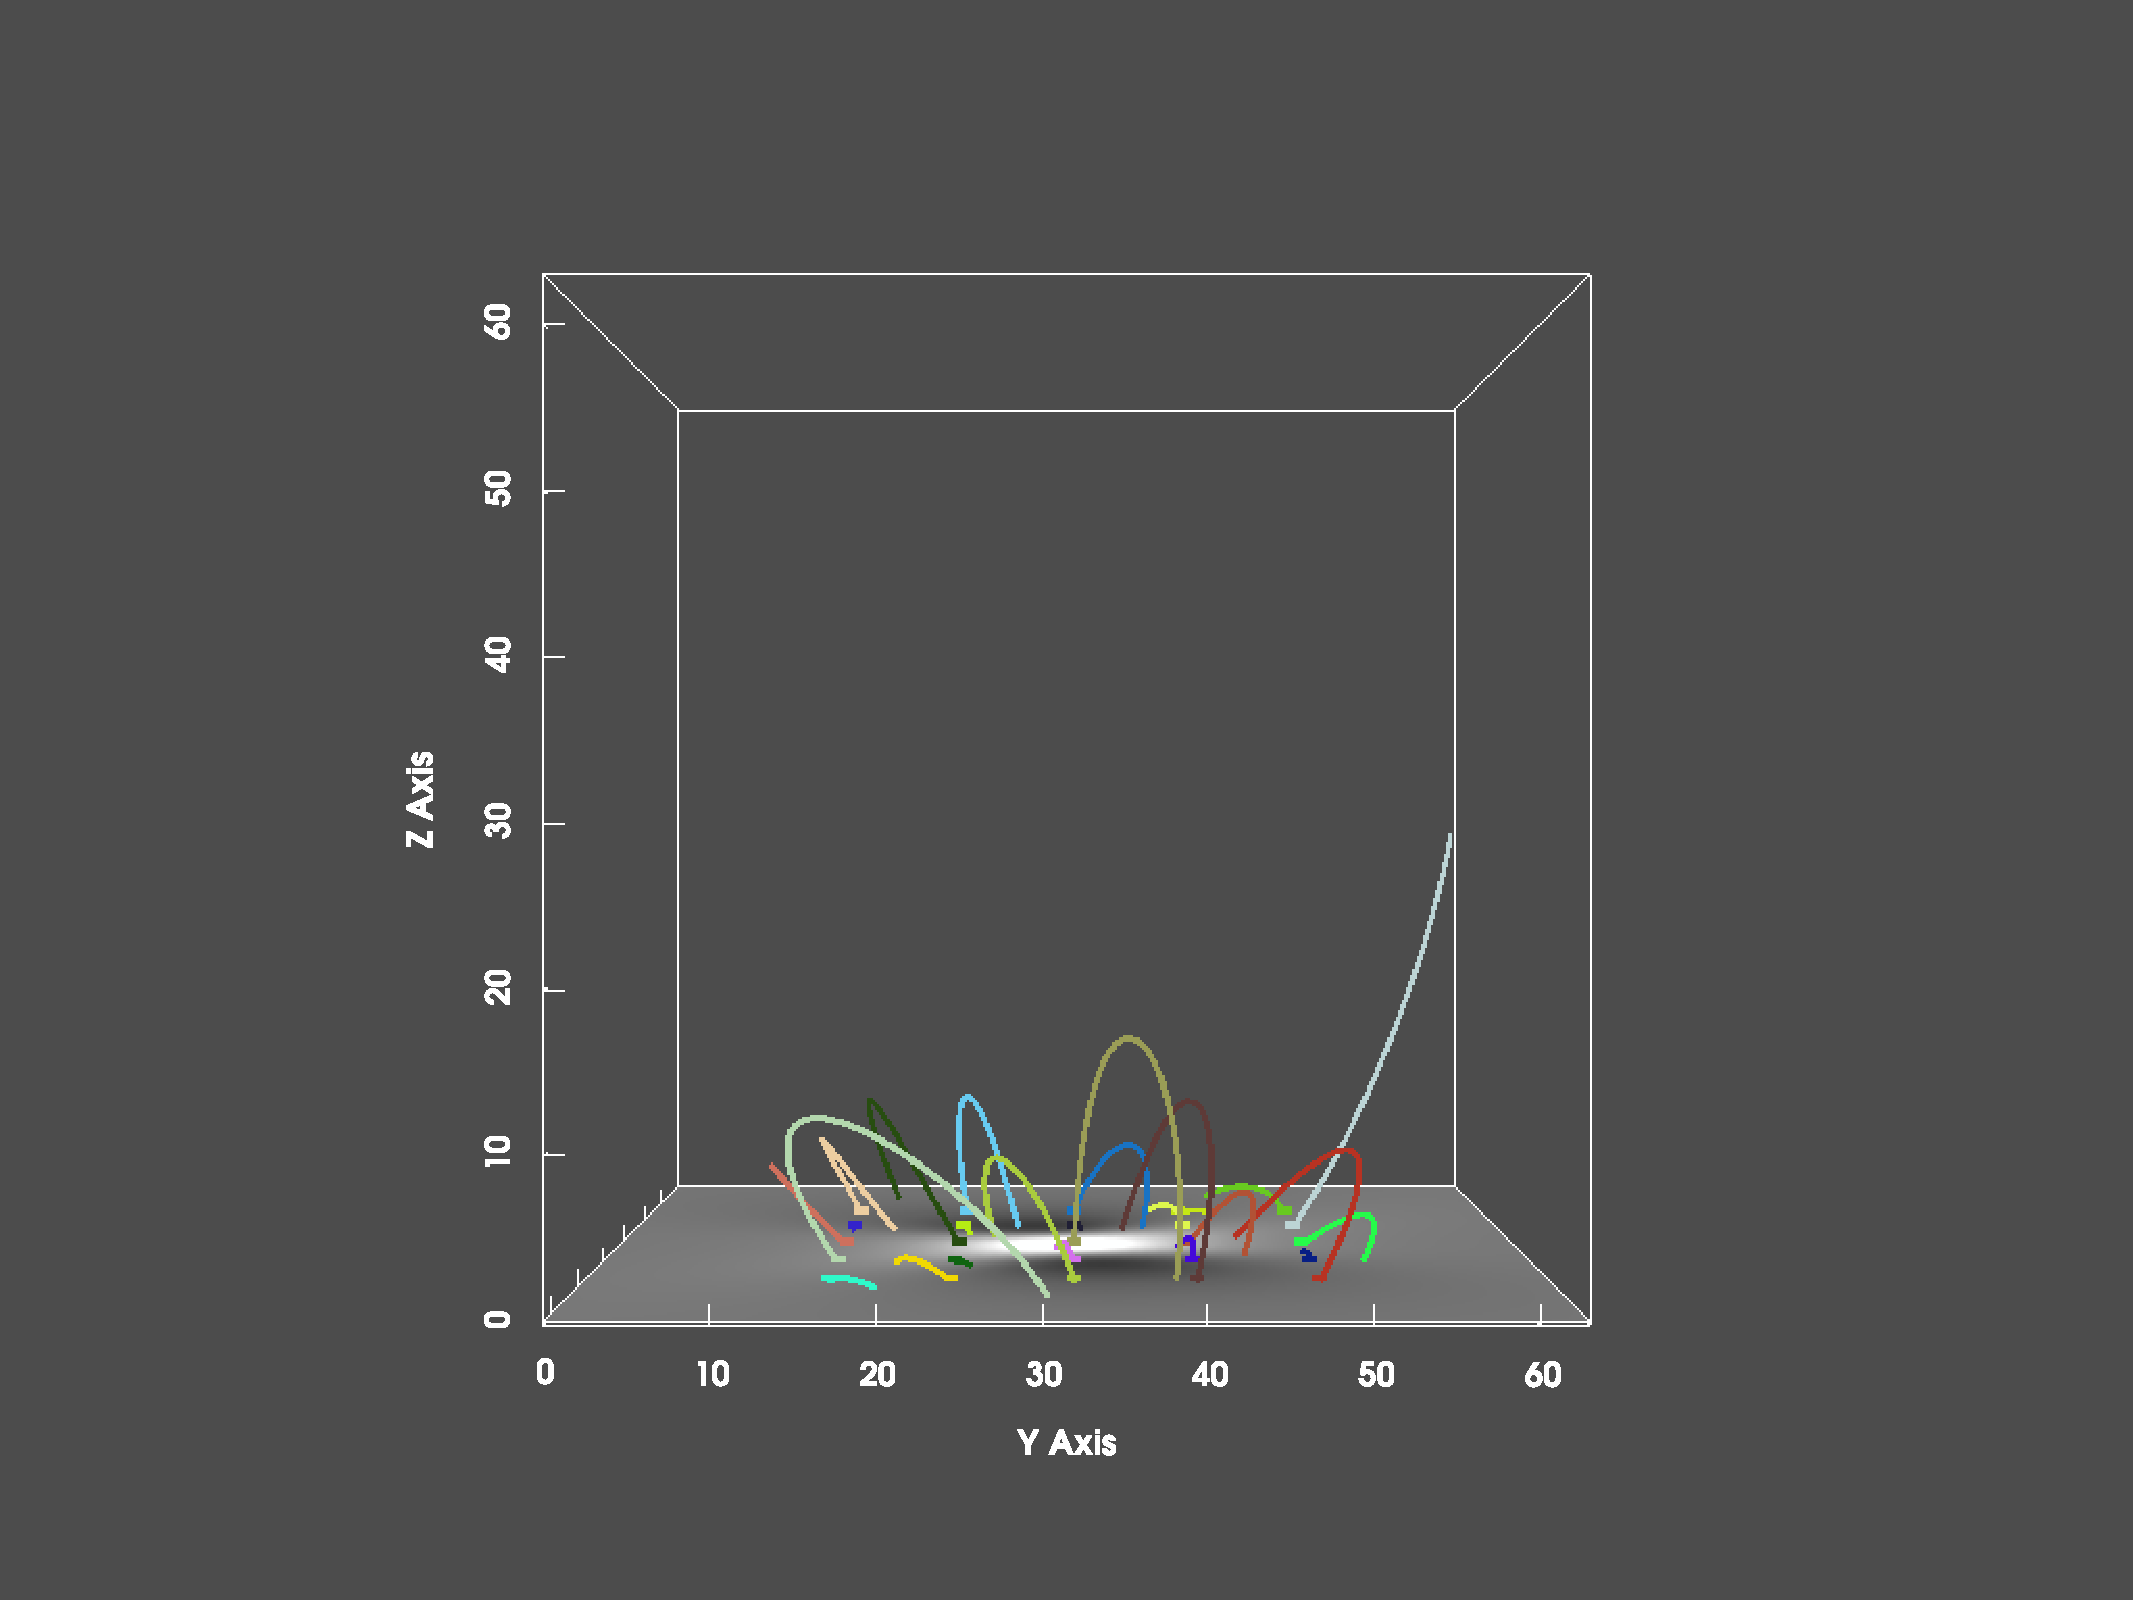
\includegraphics[trim={6cm 1cm 6cm 2cm}, clip, width=\linewidth]{"img/LL_pot_yz.pdf"}
  \end{subfigure}%
  \begin{subfigure}{.5\linewidth}
    \centering
    \caption{Low-Lou}
    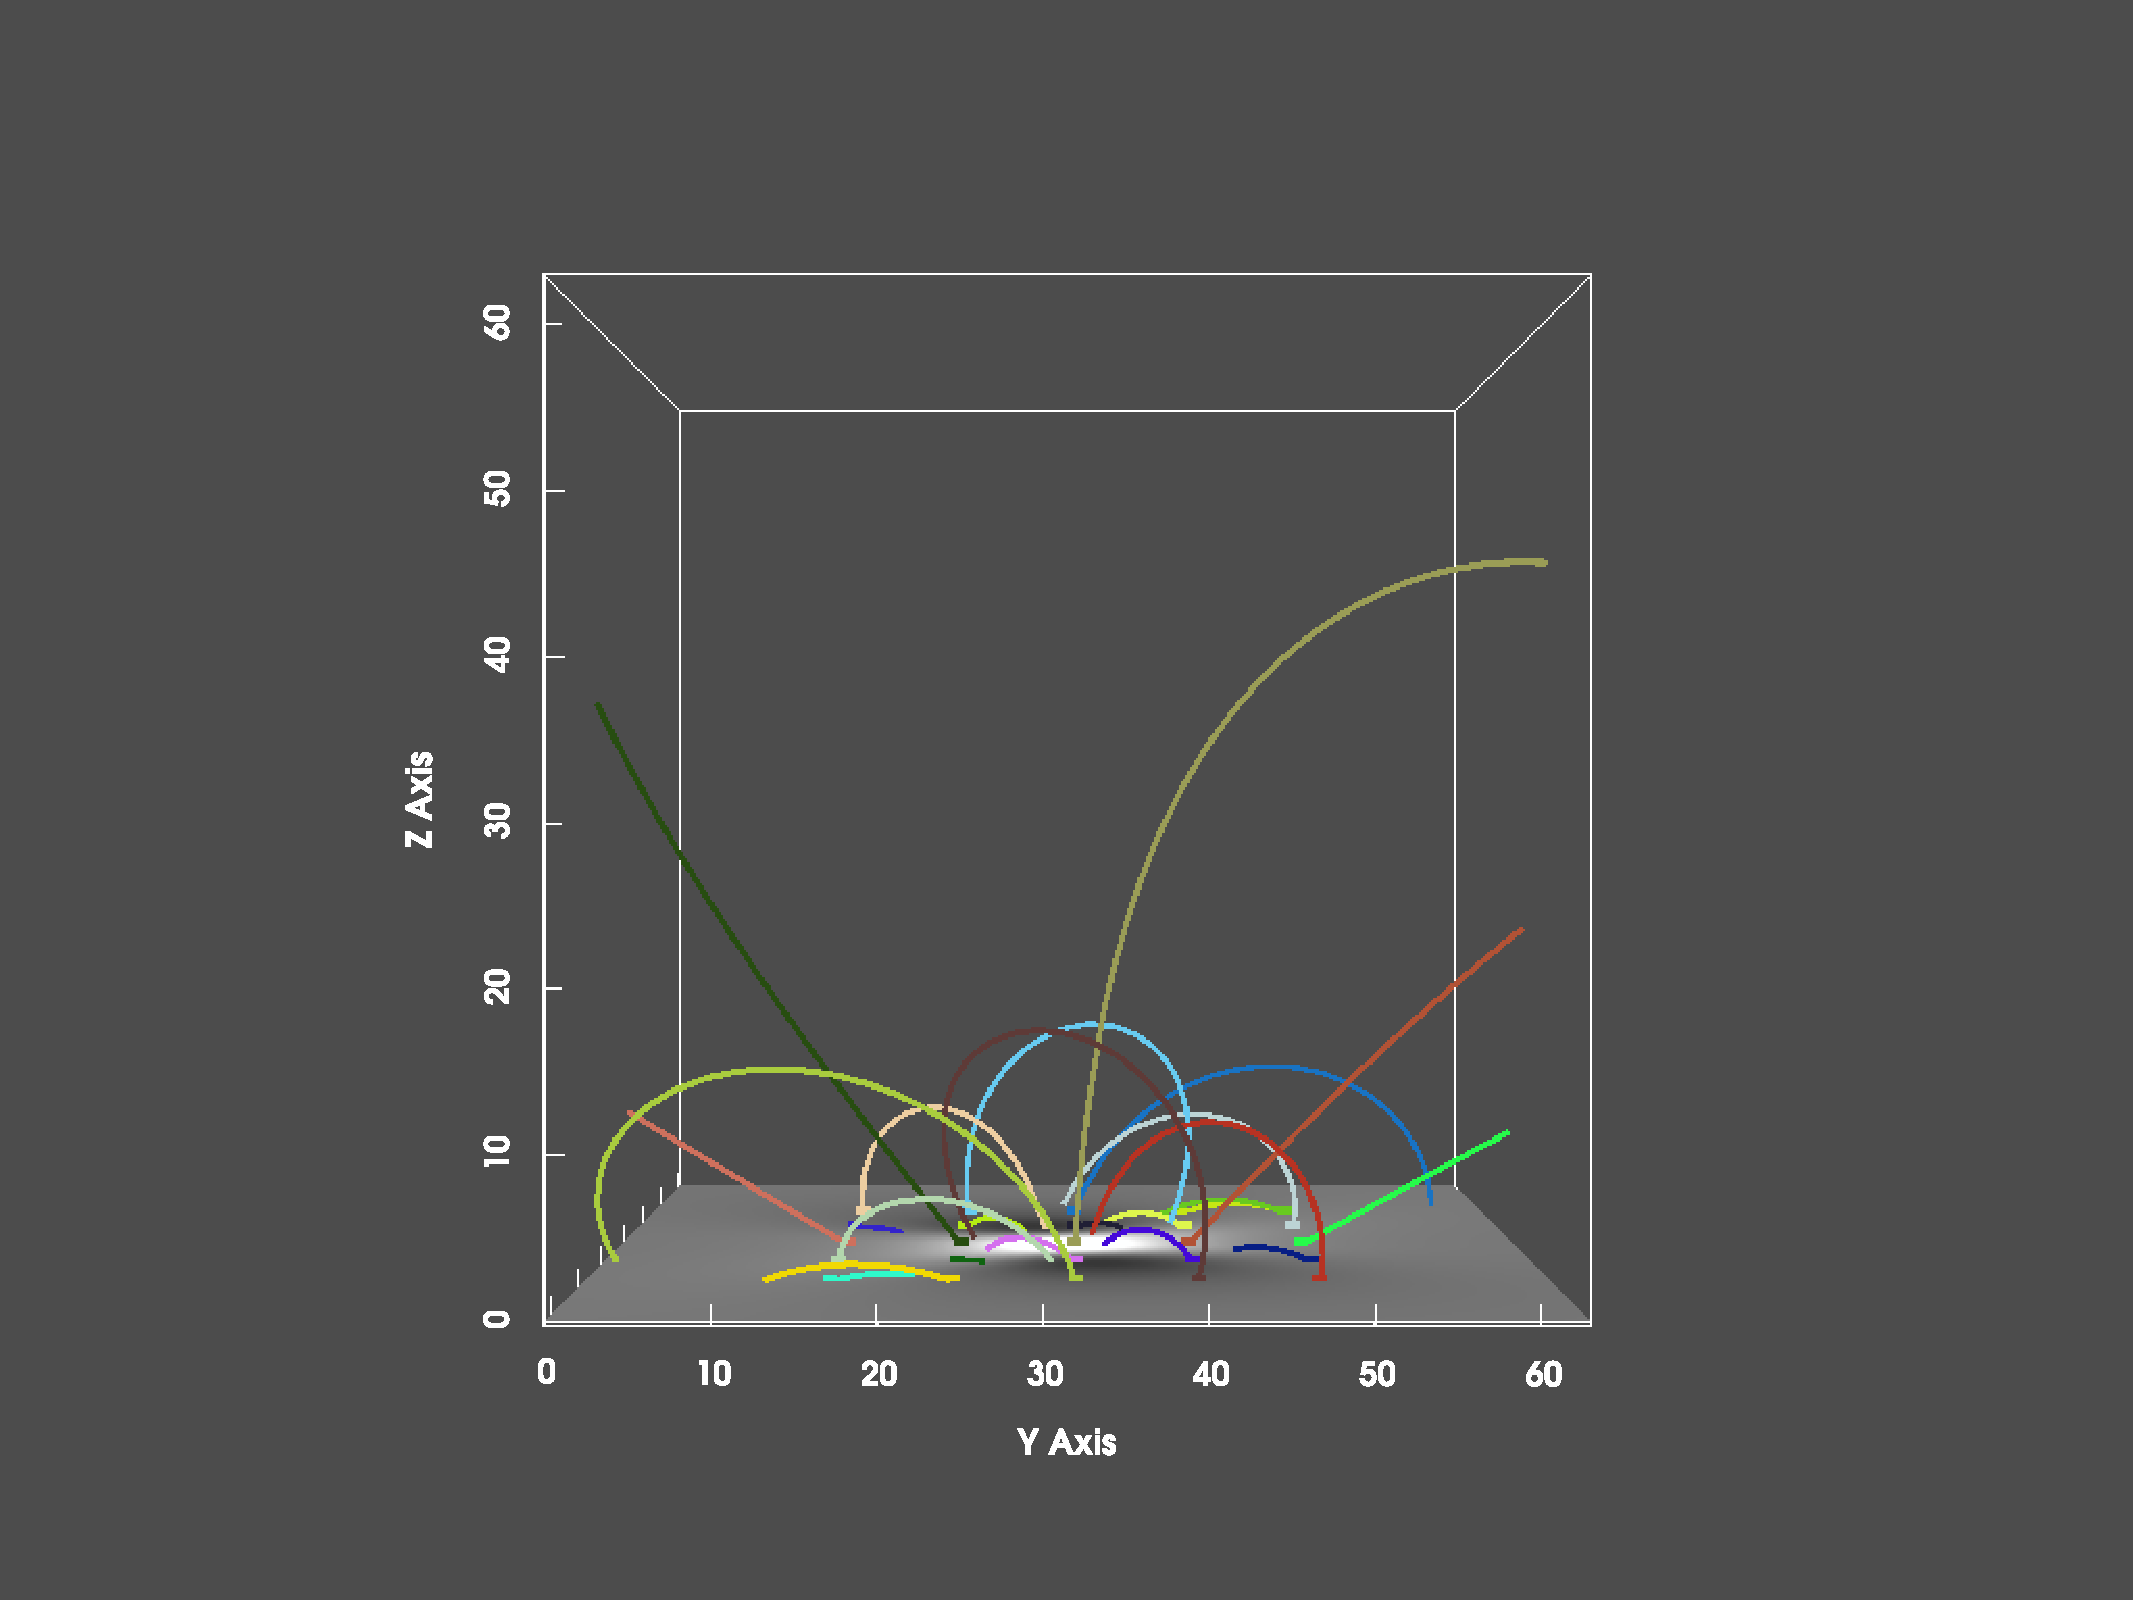
\includegraphics[trim={6cm 1cm 6cm 2cm}, clip, width=\linewidth]{"img/LL_yz.pdf"}
  \end{subfigure}
  
  \caption{The magnetic fields in the yz plane. Each field line is distinguished by its unique color, which is determined by its footpoint at $z=0$ plane.}\label{fig:yz}
\end{figure}

\begin{figure}
  \begin{subfigure}{.5\linewidth}
    \centering
    \caption{PINN(0)}\label{fig:xz0}
    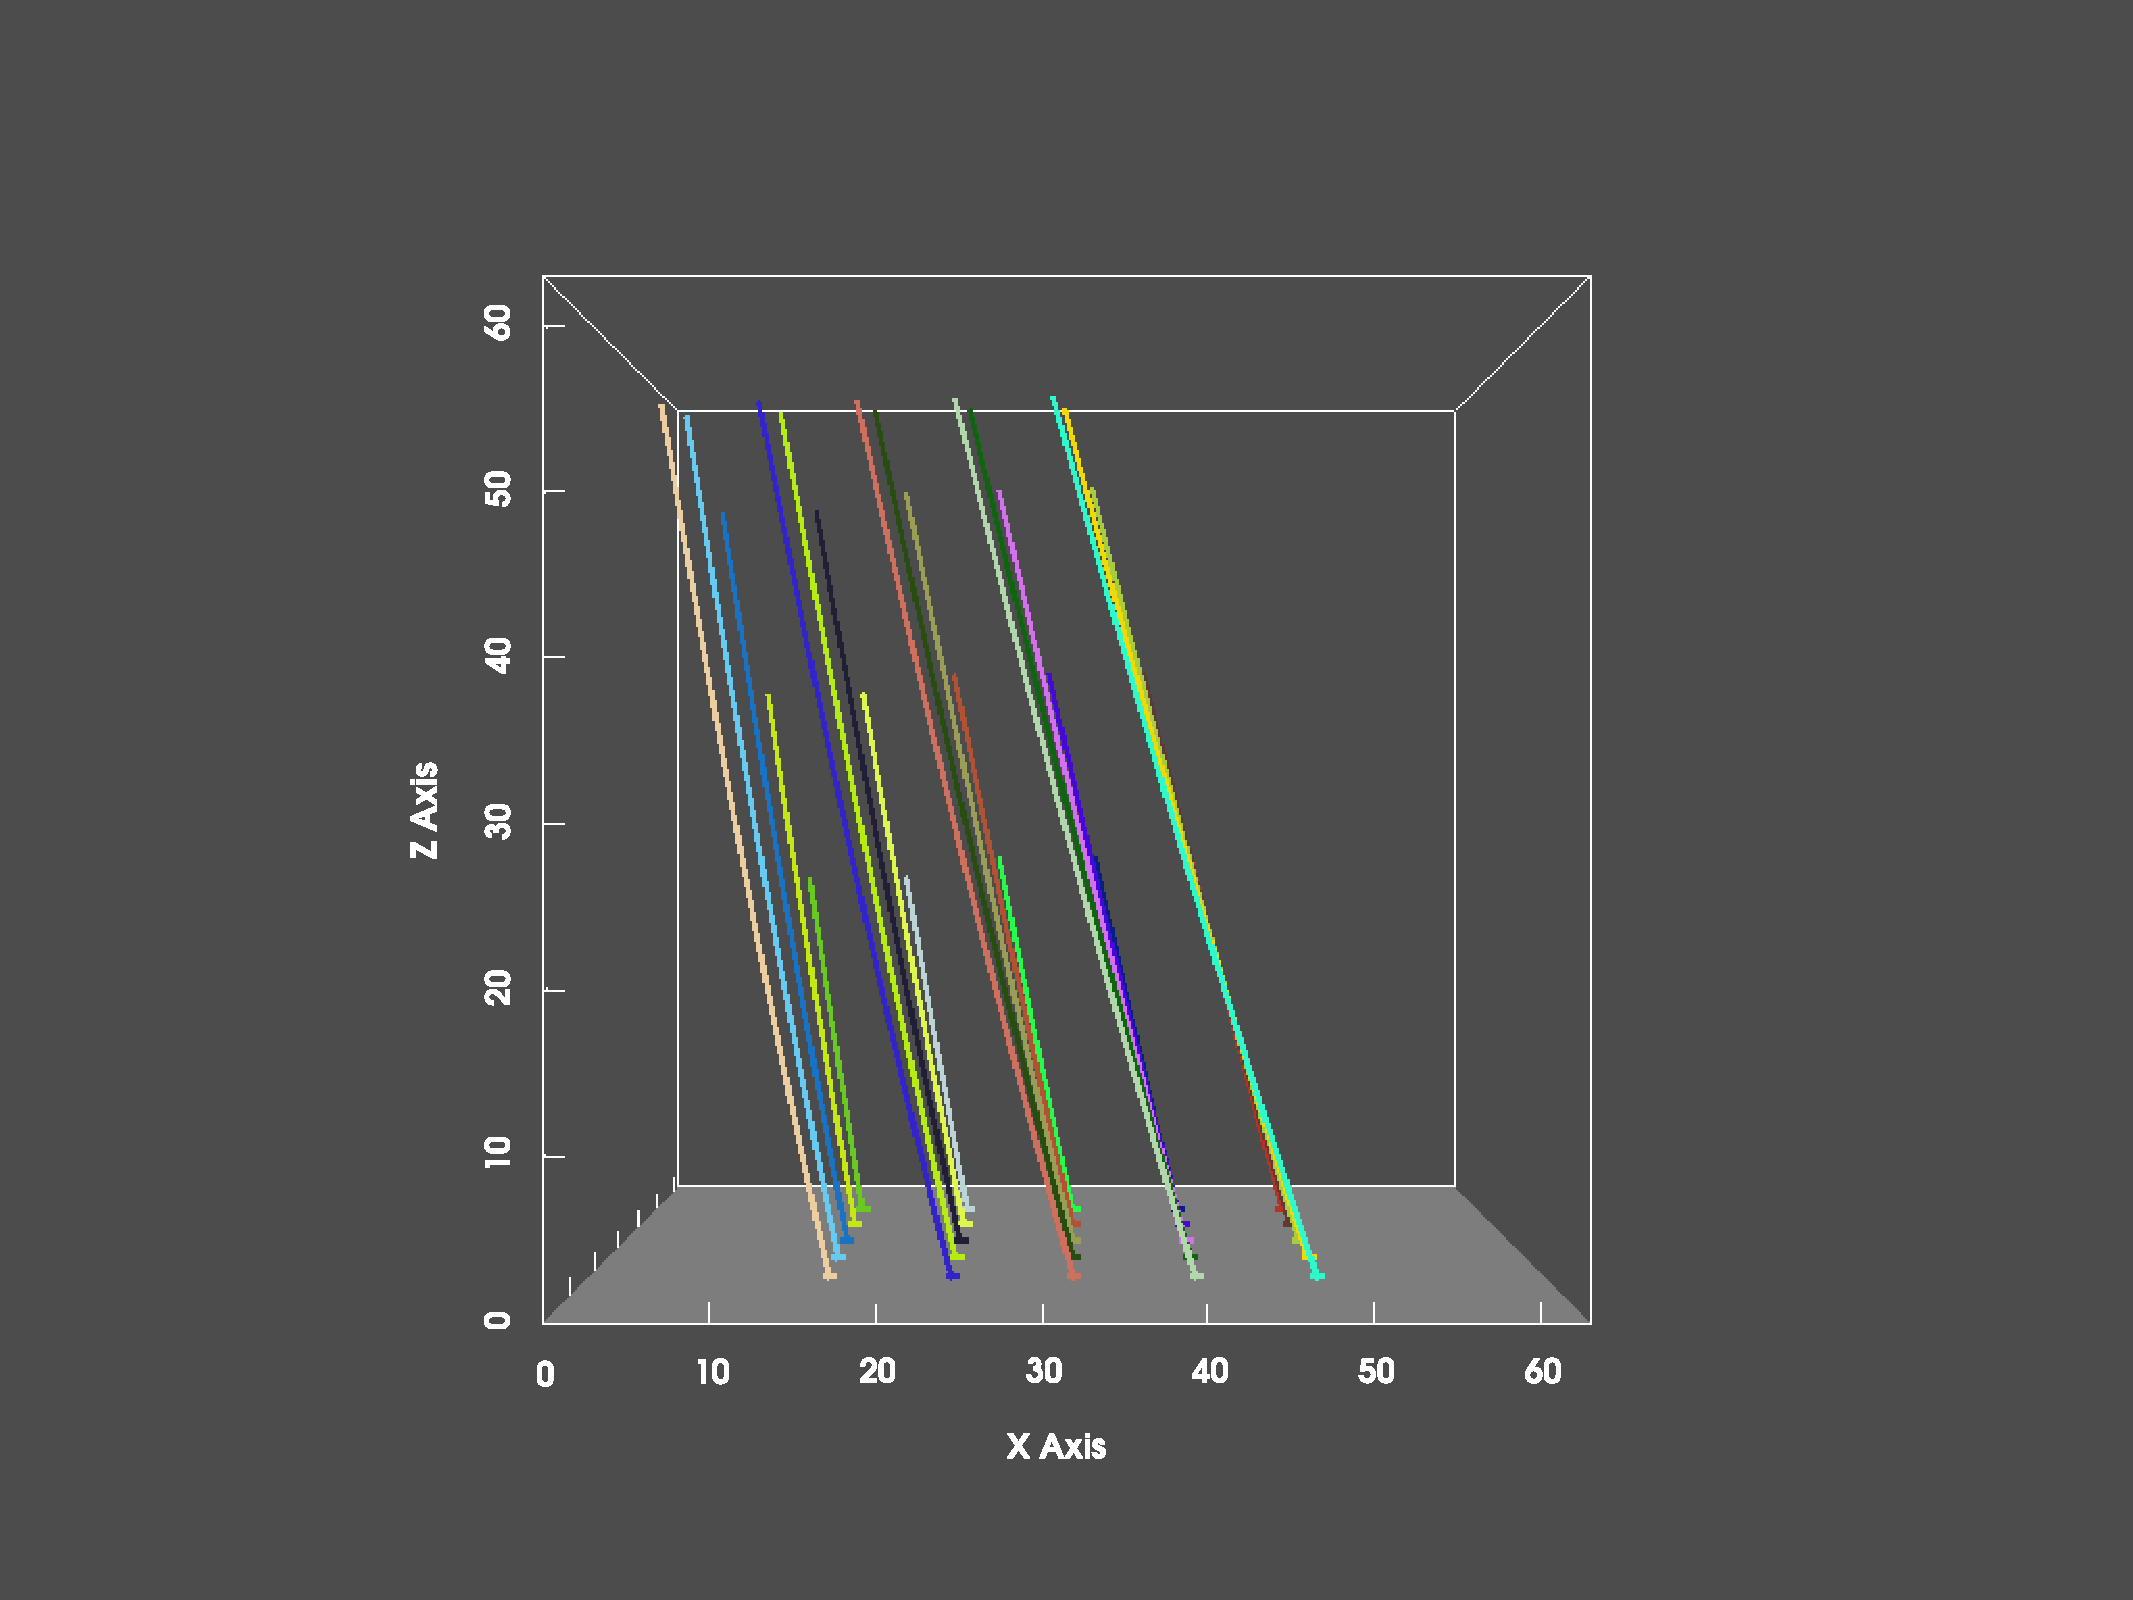
\includegraphics[trim={6cm 1cm 6cm 2cm}, clip, width=\linewidth]{"img/PINN_000000_xz.pdf"}
  \end{subfigure}%
  \begin{subfigure}{.5\linewidth}
    \centering
    \caption{PINN(100)}
    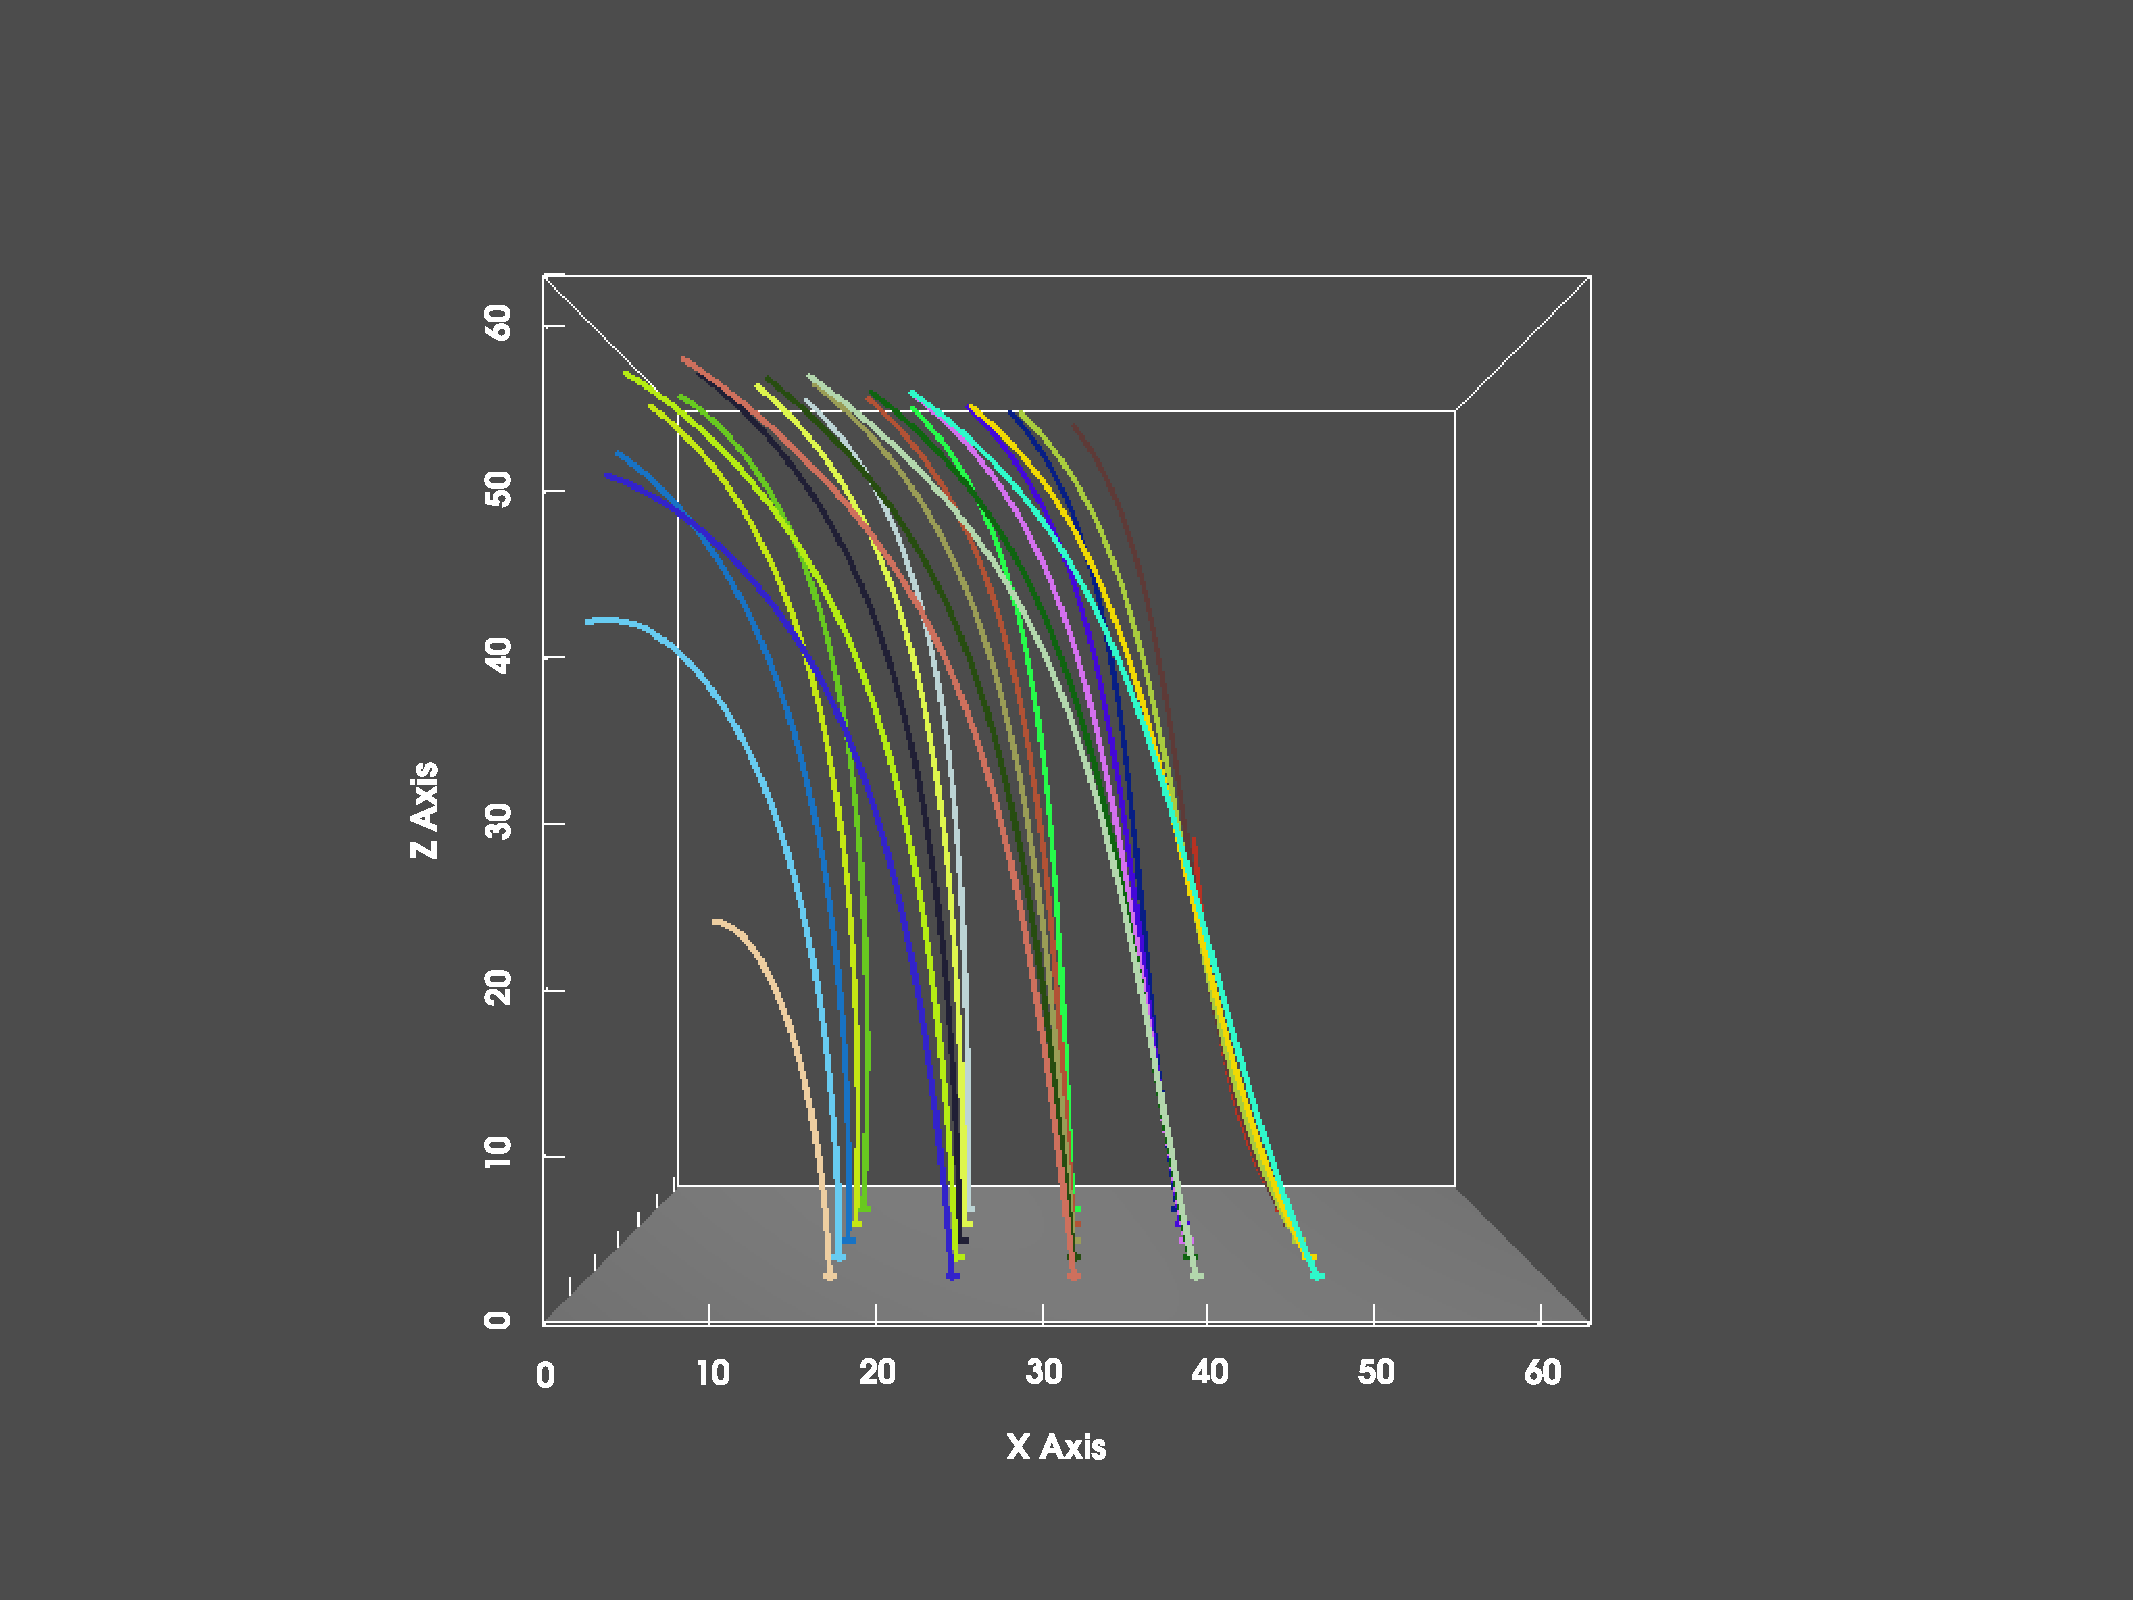
\includegraphics[trim={6cm 1cm 6cm 2cm}, clip, width=\linewidth]{"img/PINN_000100_xz.pdf"}
  \end{subfigure}

  \begin{subfigure}{.5\linewidth}
    \centering
    \caption{PINN(1000)}
    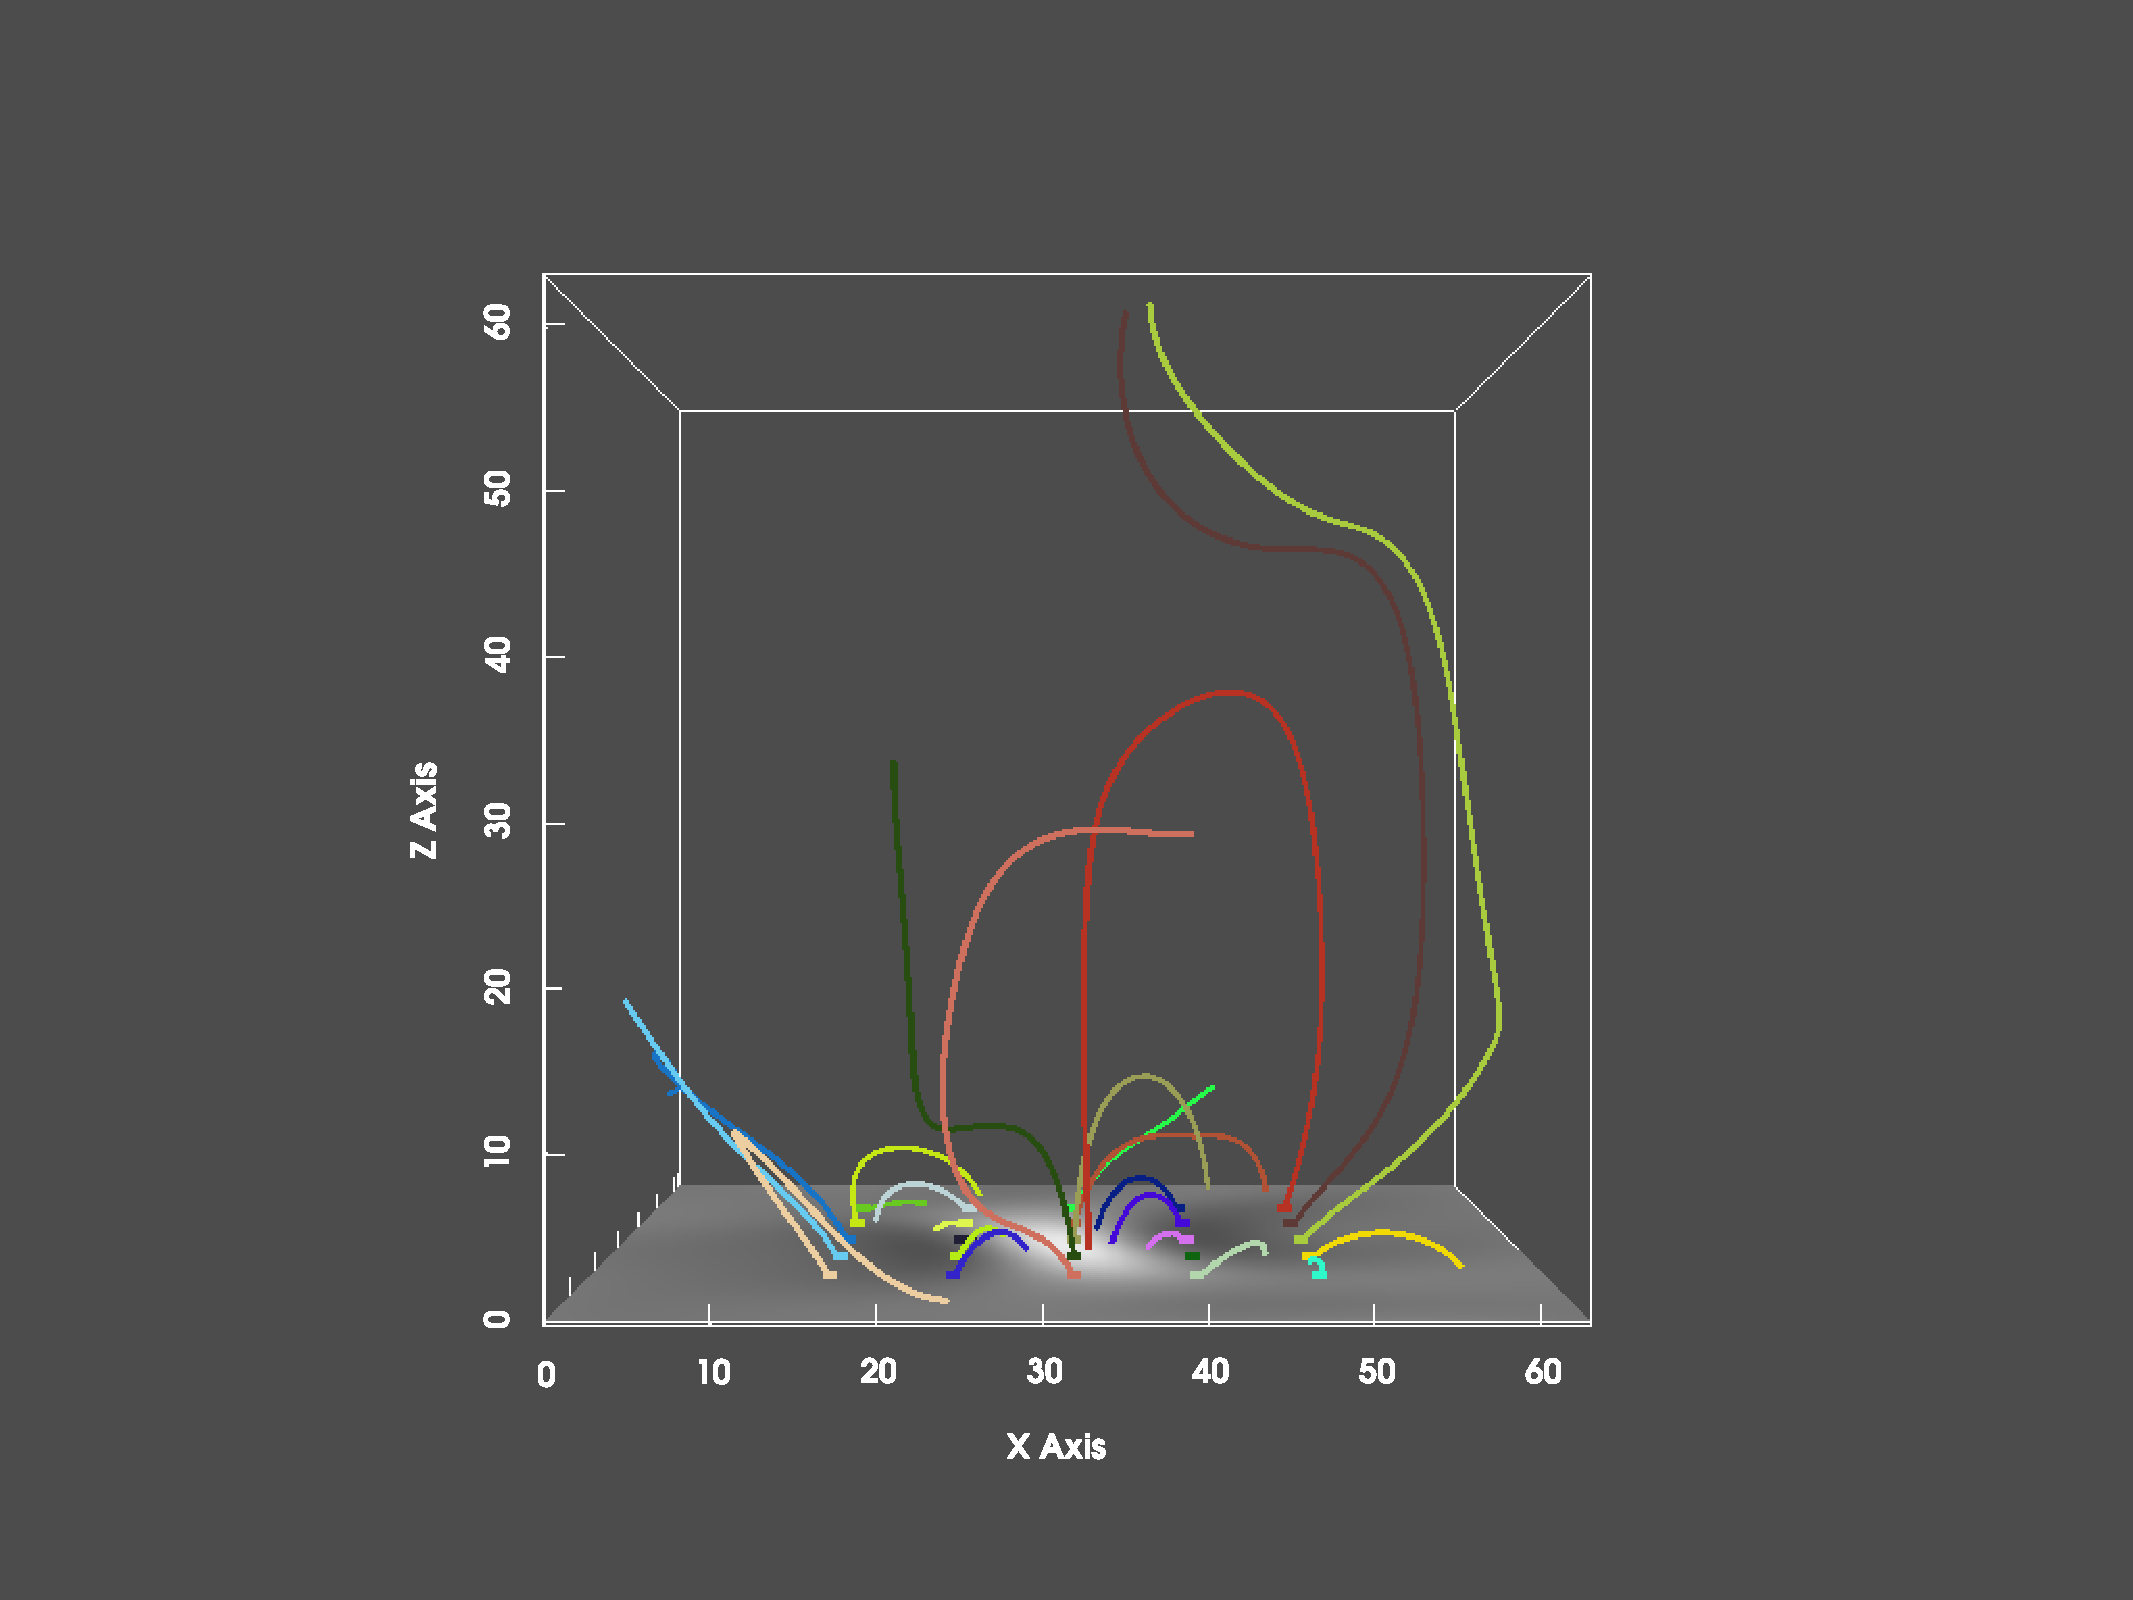
\includegraphics[trim={6cm 1cm 6cm 2cm}, clip, width=\linewidth]{"img/PINN_001000_xz.pdf"}
  \end{subfigure}%
  \begin{subfigure}{.5\linewidth}
    \centering
    \caption{PINN(10000)}
    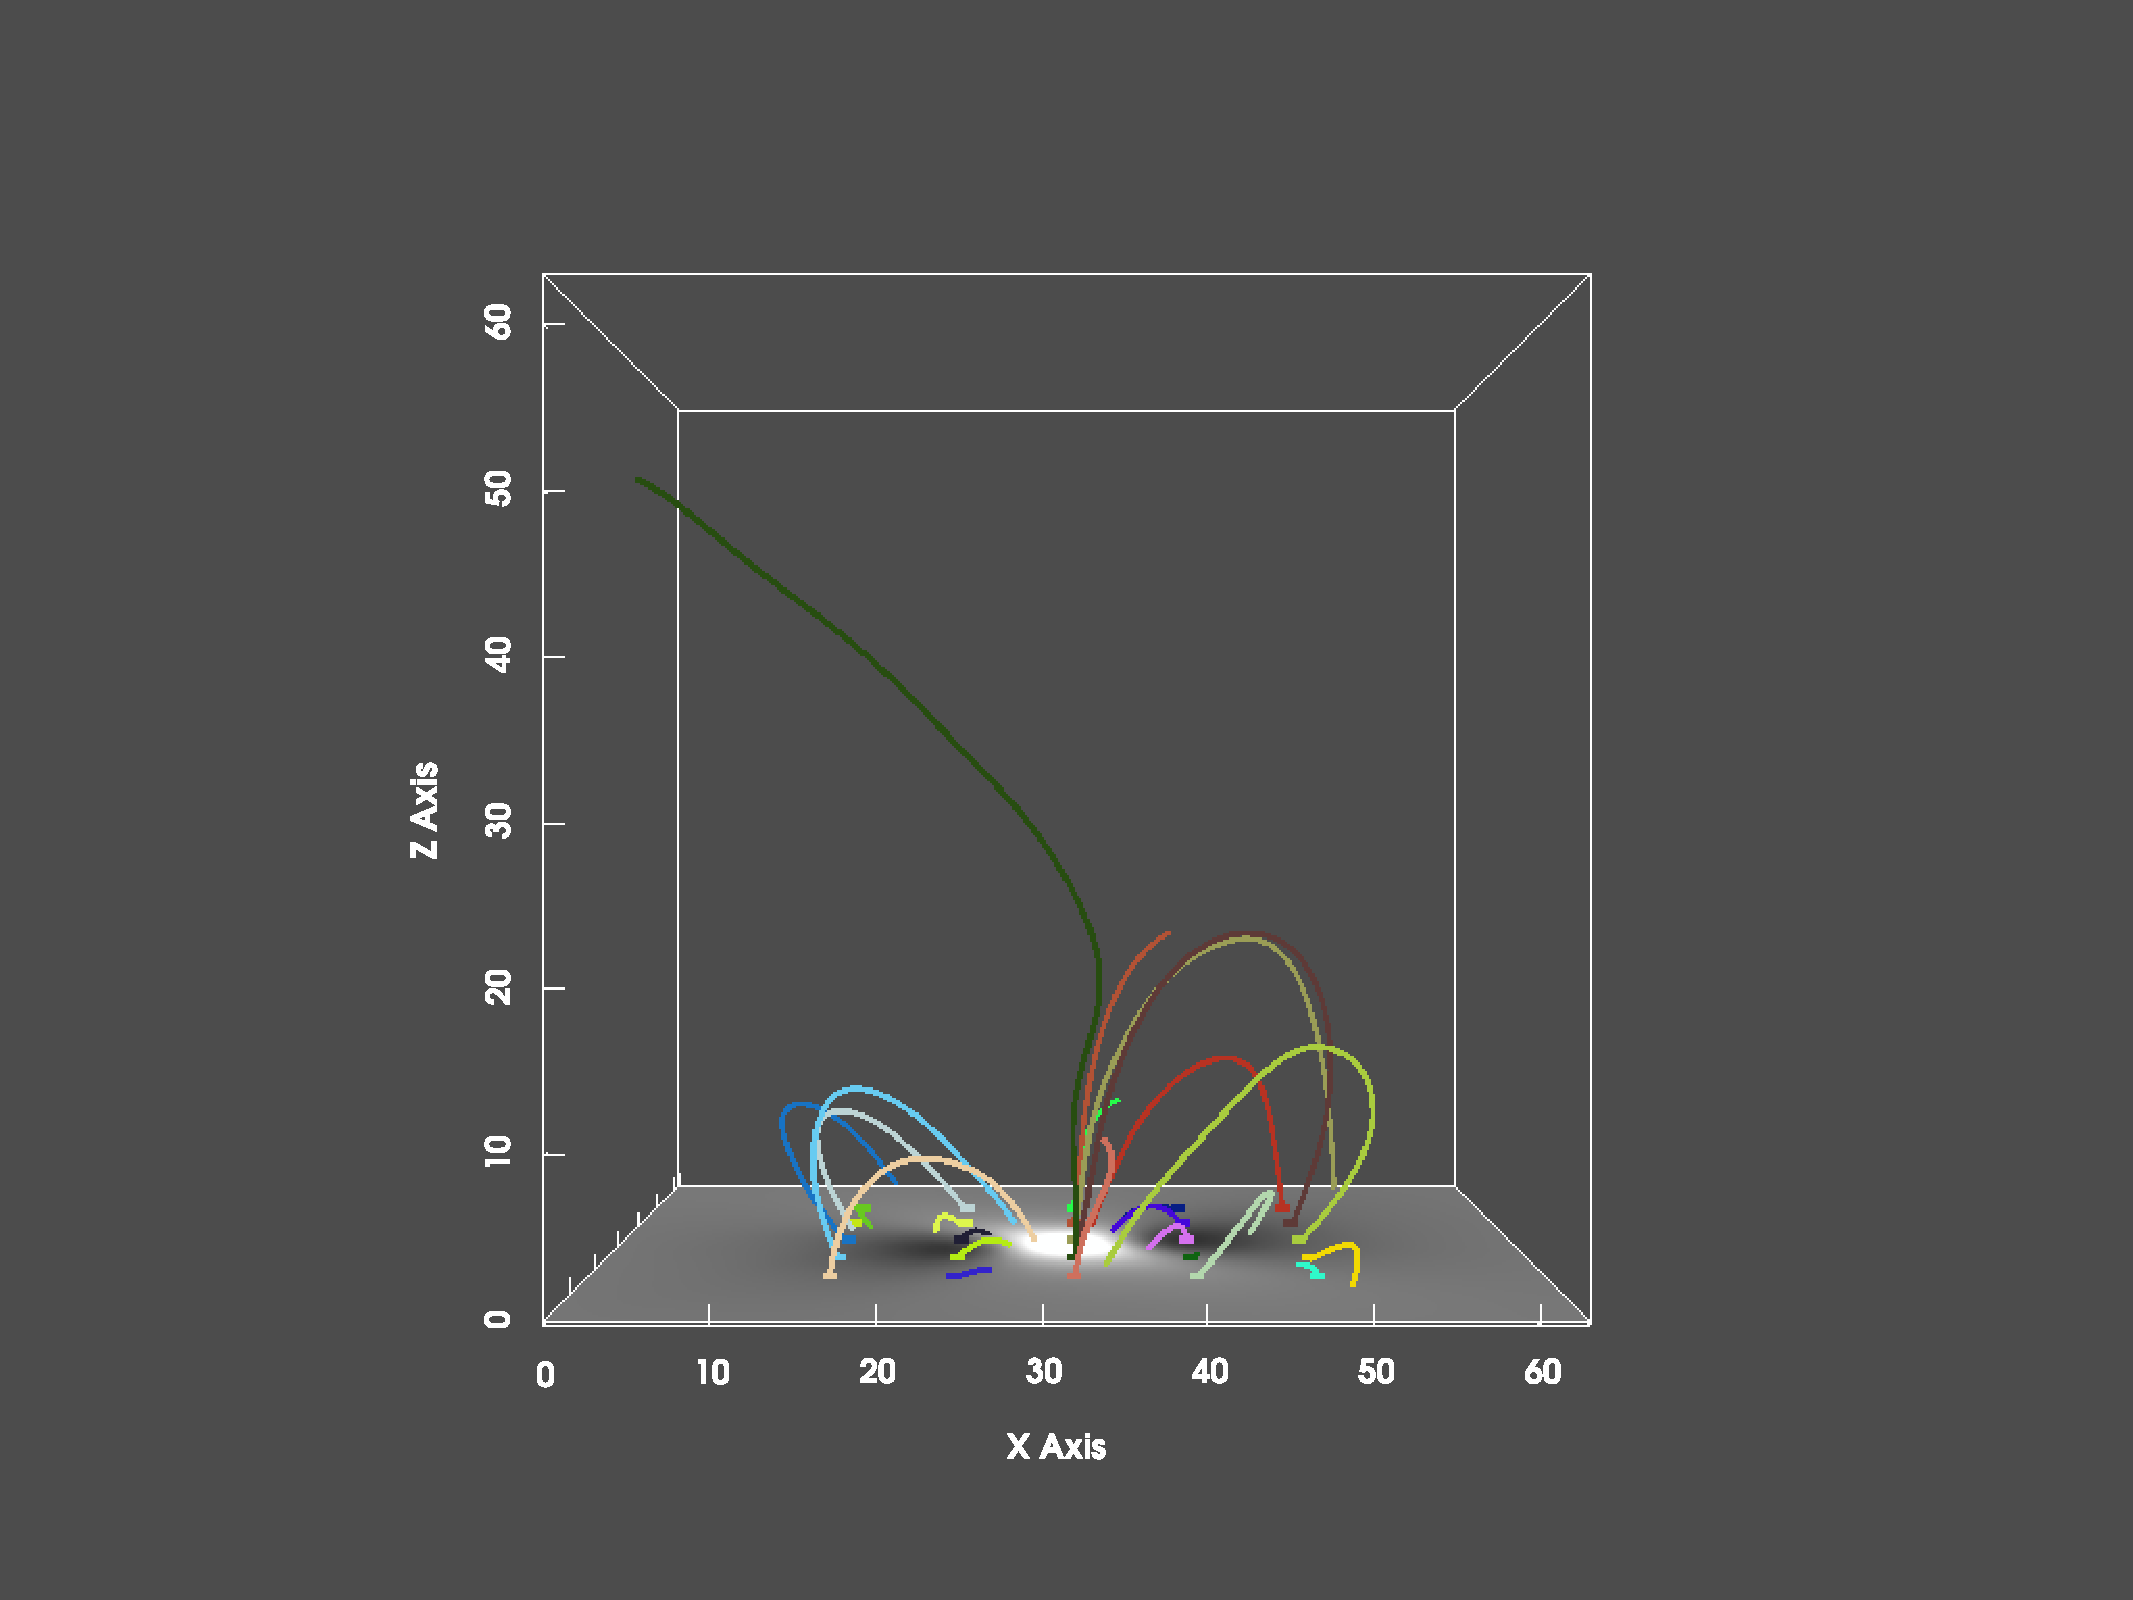
\includegraphics[trim={6cm 1cm 6cm 2cm}, clip, width=\linewidth]{"img/PINN_010000_xz.pdf"}
  \end{subfigure}

  \begin{subfigure}{.5\linewidth}
    \centering
    \caption{PINN(25000)}
    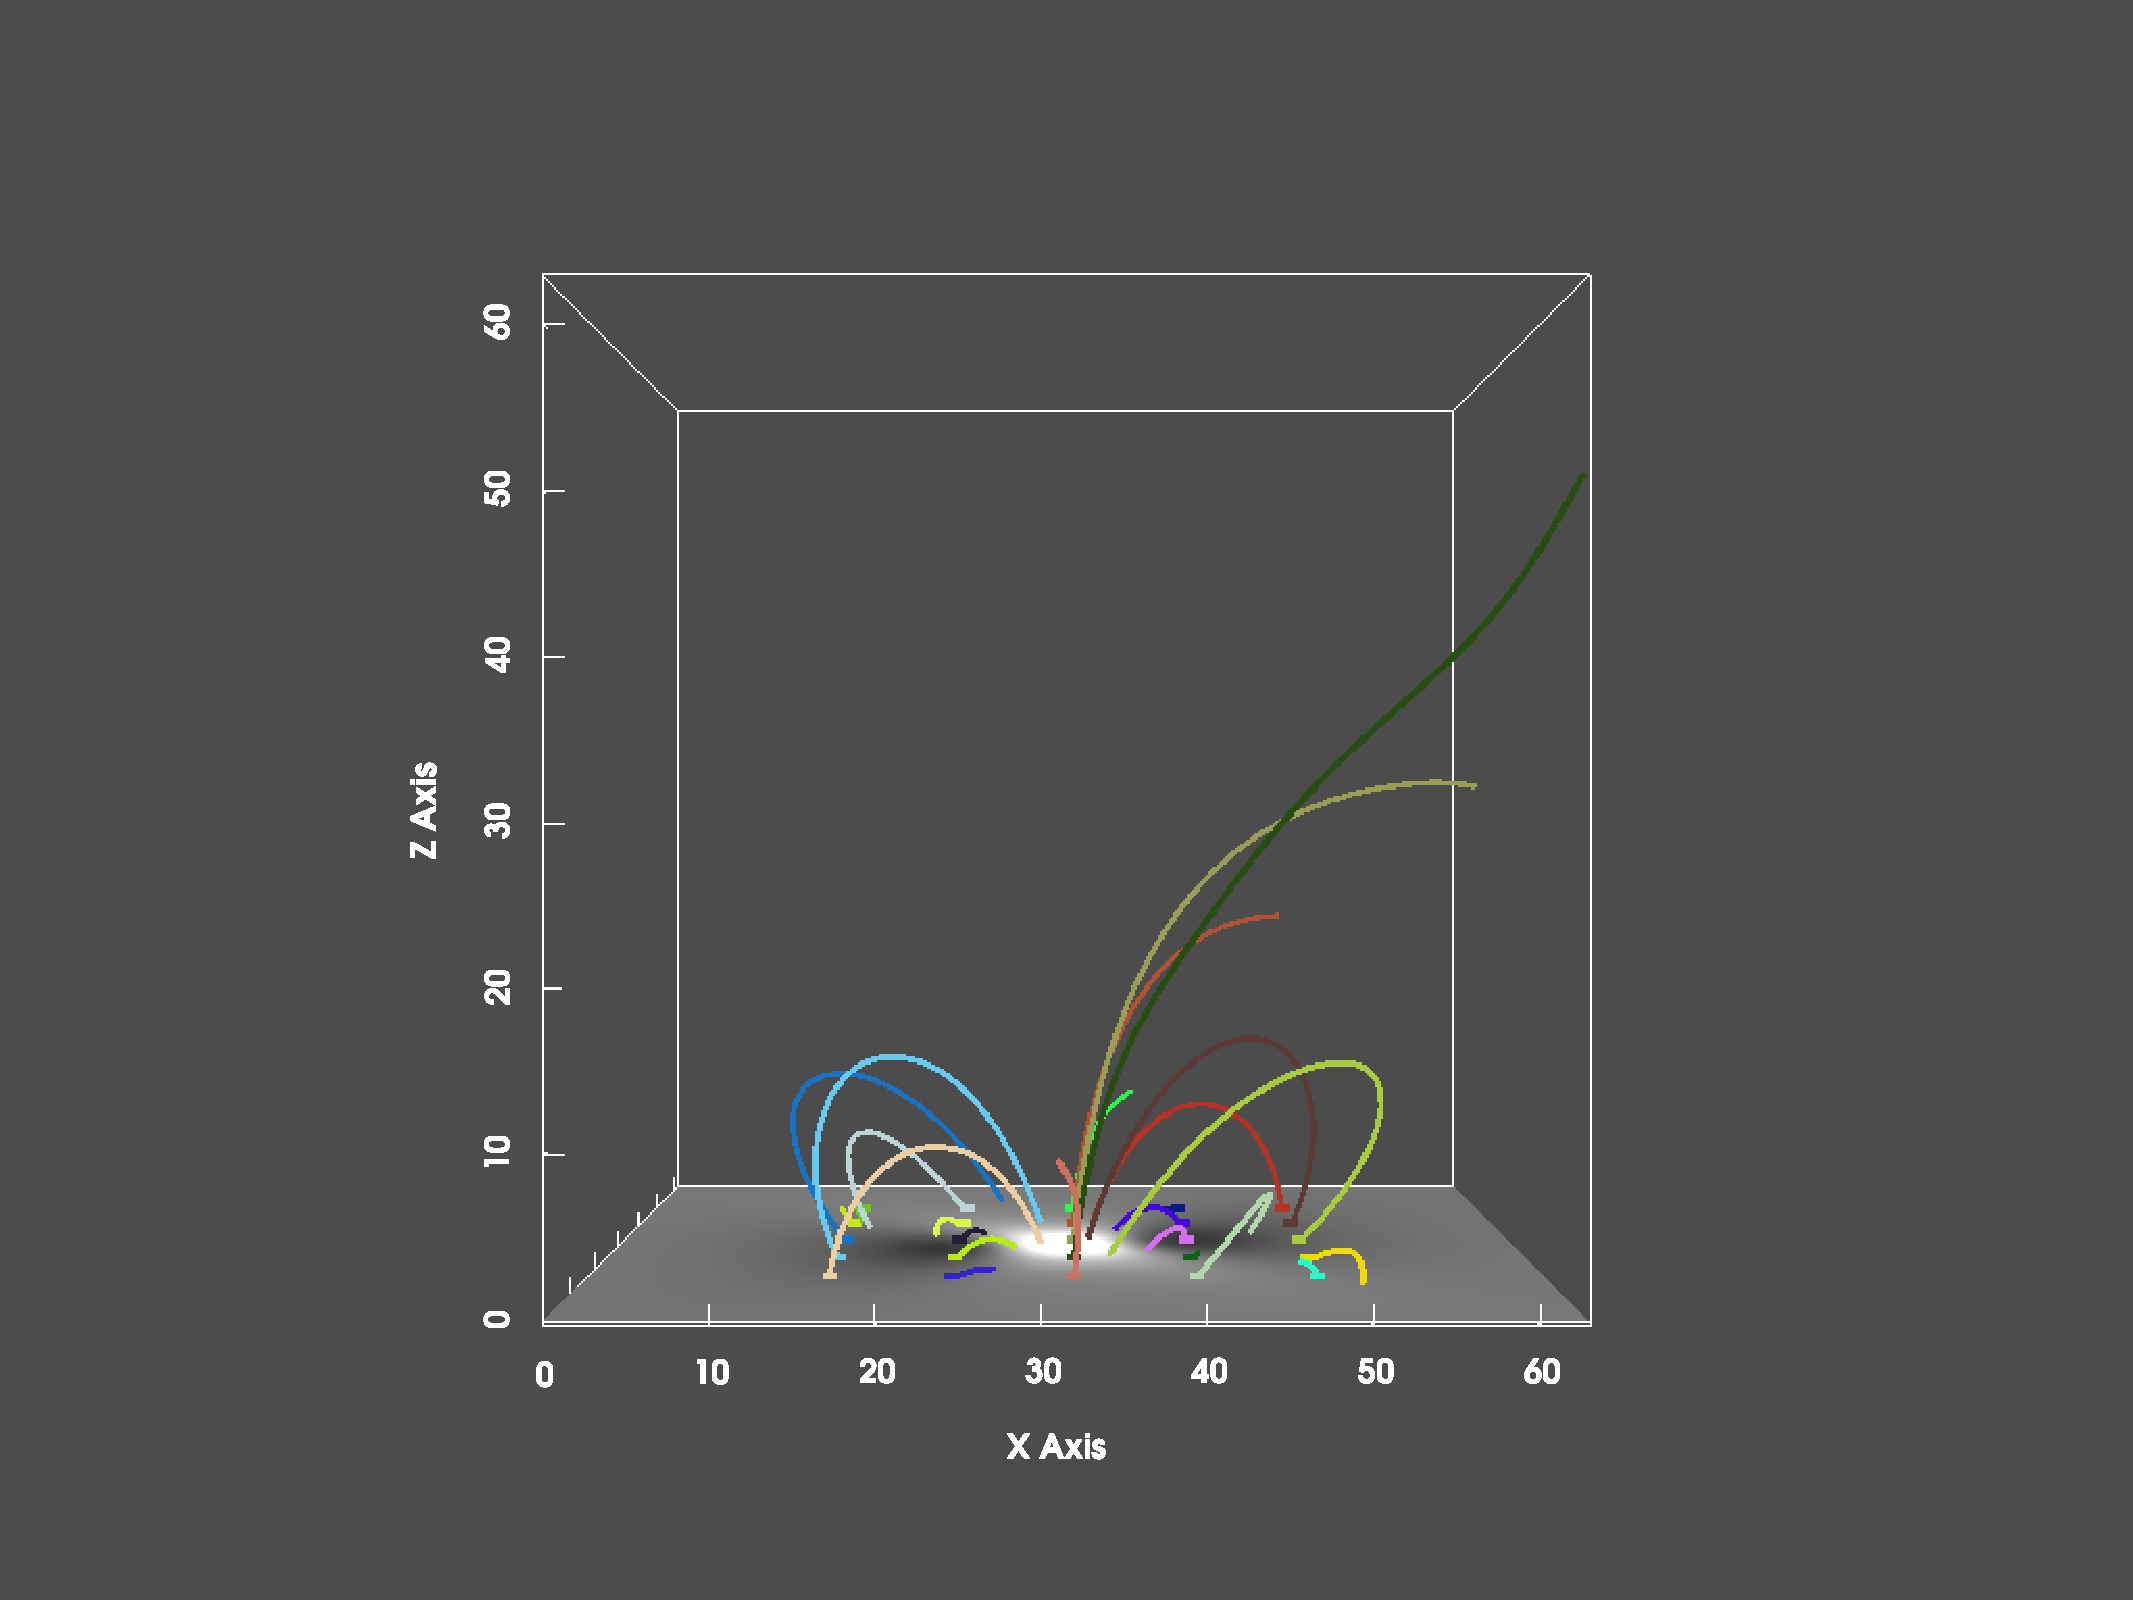
\includegraphics[trim={6cm 1cm 6cm 2cm}, clip, width=\linewidth]{"img/PINN_025000_xz.pdf"}
  \end{subfigure}%
  \begin{subfigure}{.5\linewidth}
    \centering
    \caption{PINN(50000)}
    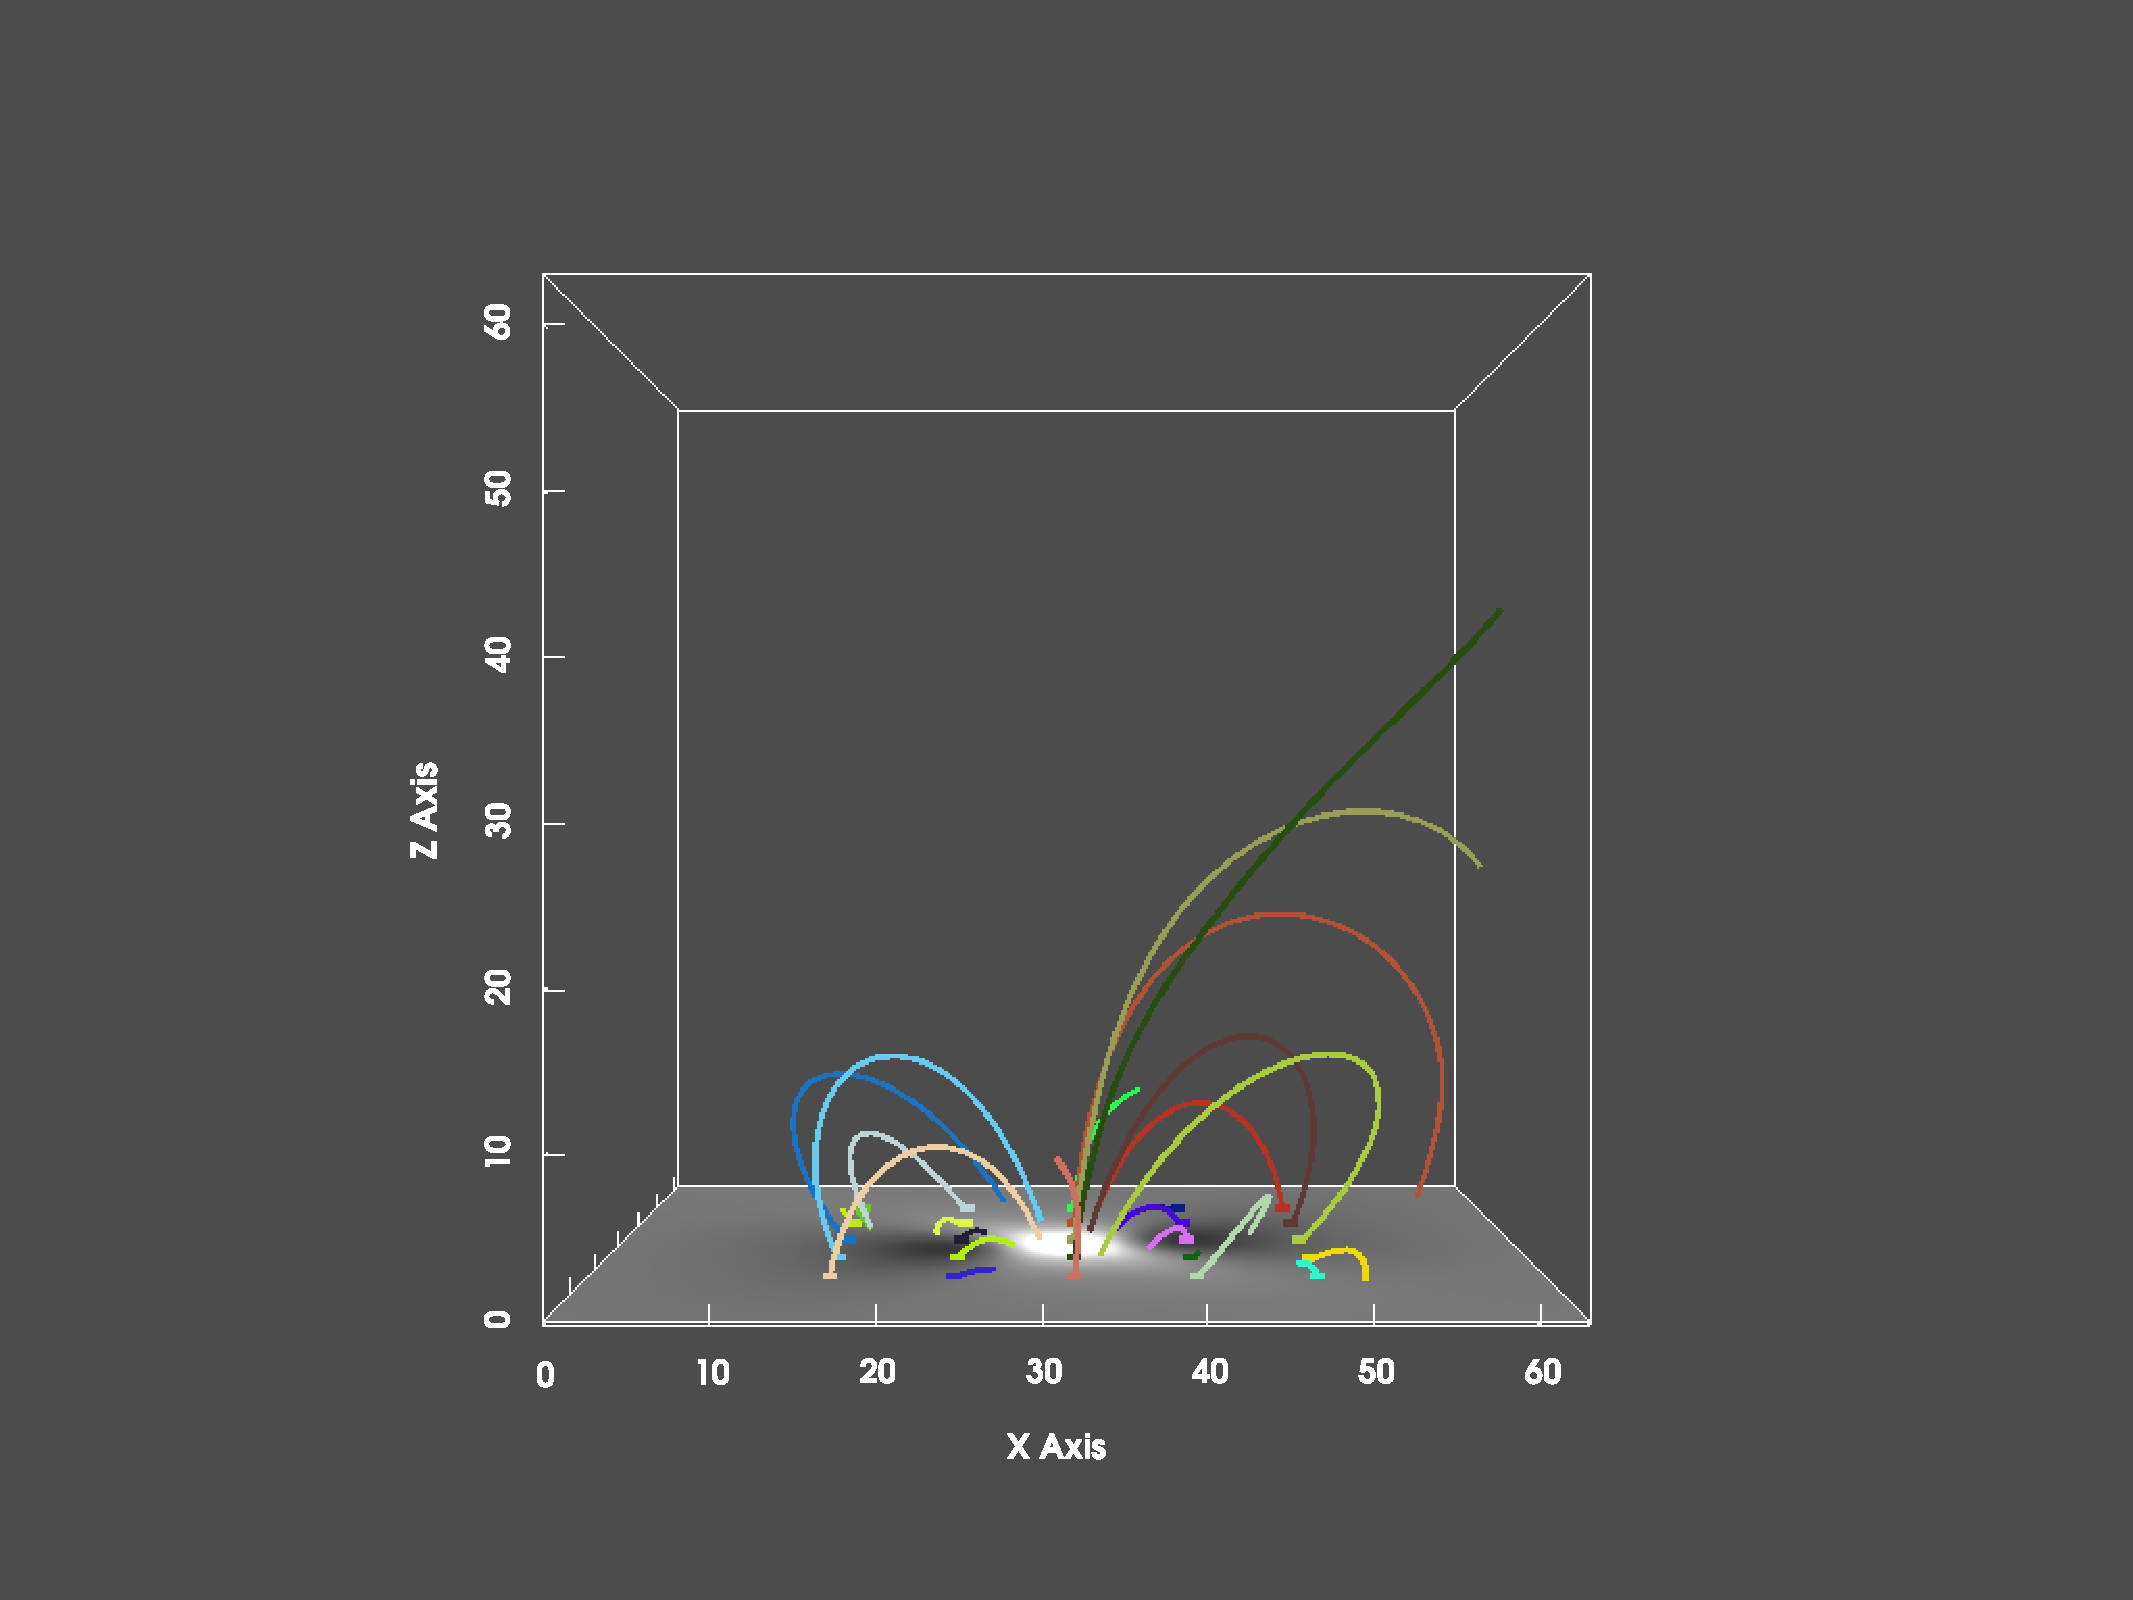
\includegraphics[trim={6cm 1cm 6cm 2cm}, clip, width=\linewidth]{"img/PINN_050000_xz.pdf"}
  \end{subfigure}
  
  \begin{subfigure}{.5\linewidth}
    \centering
    \caption{Potential}
    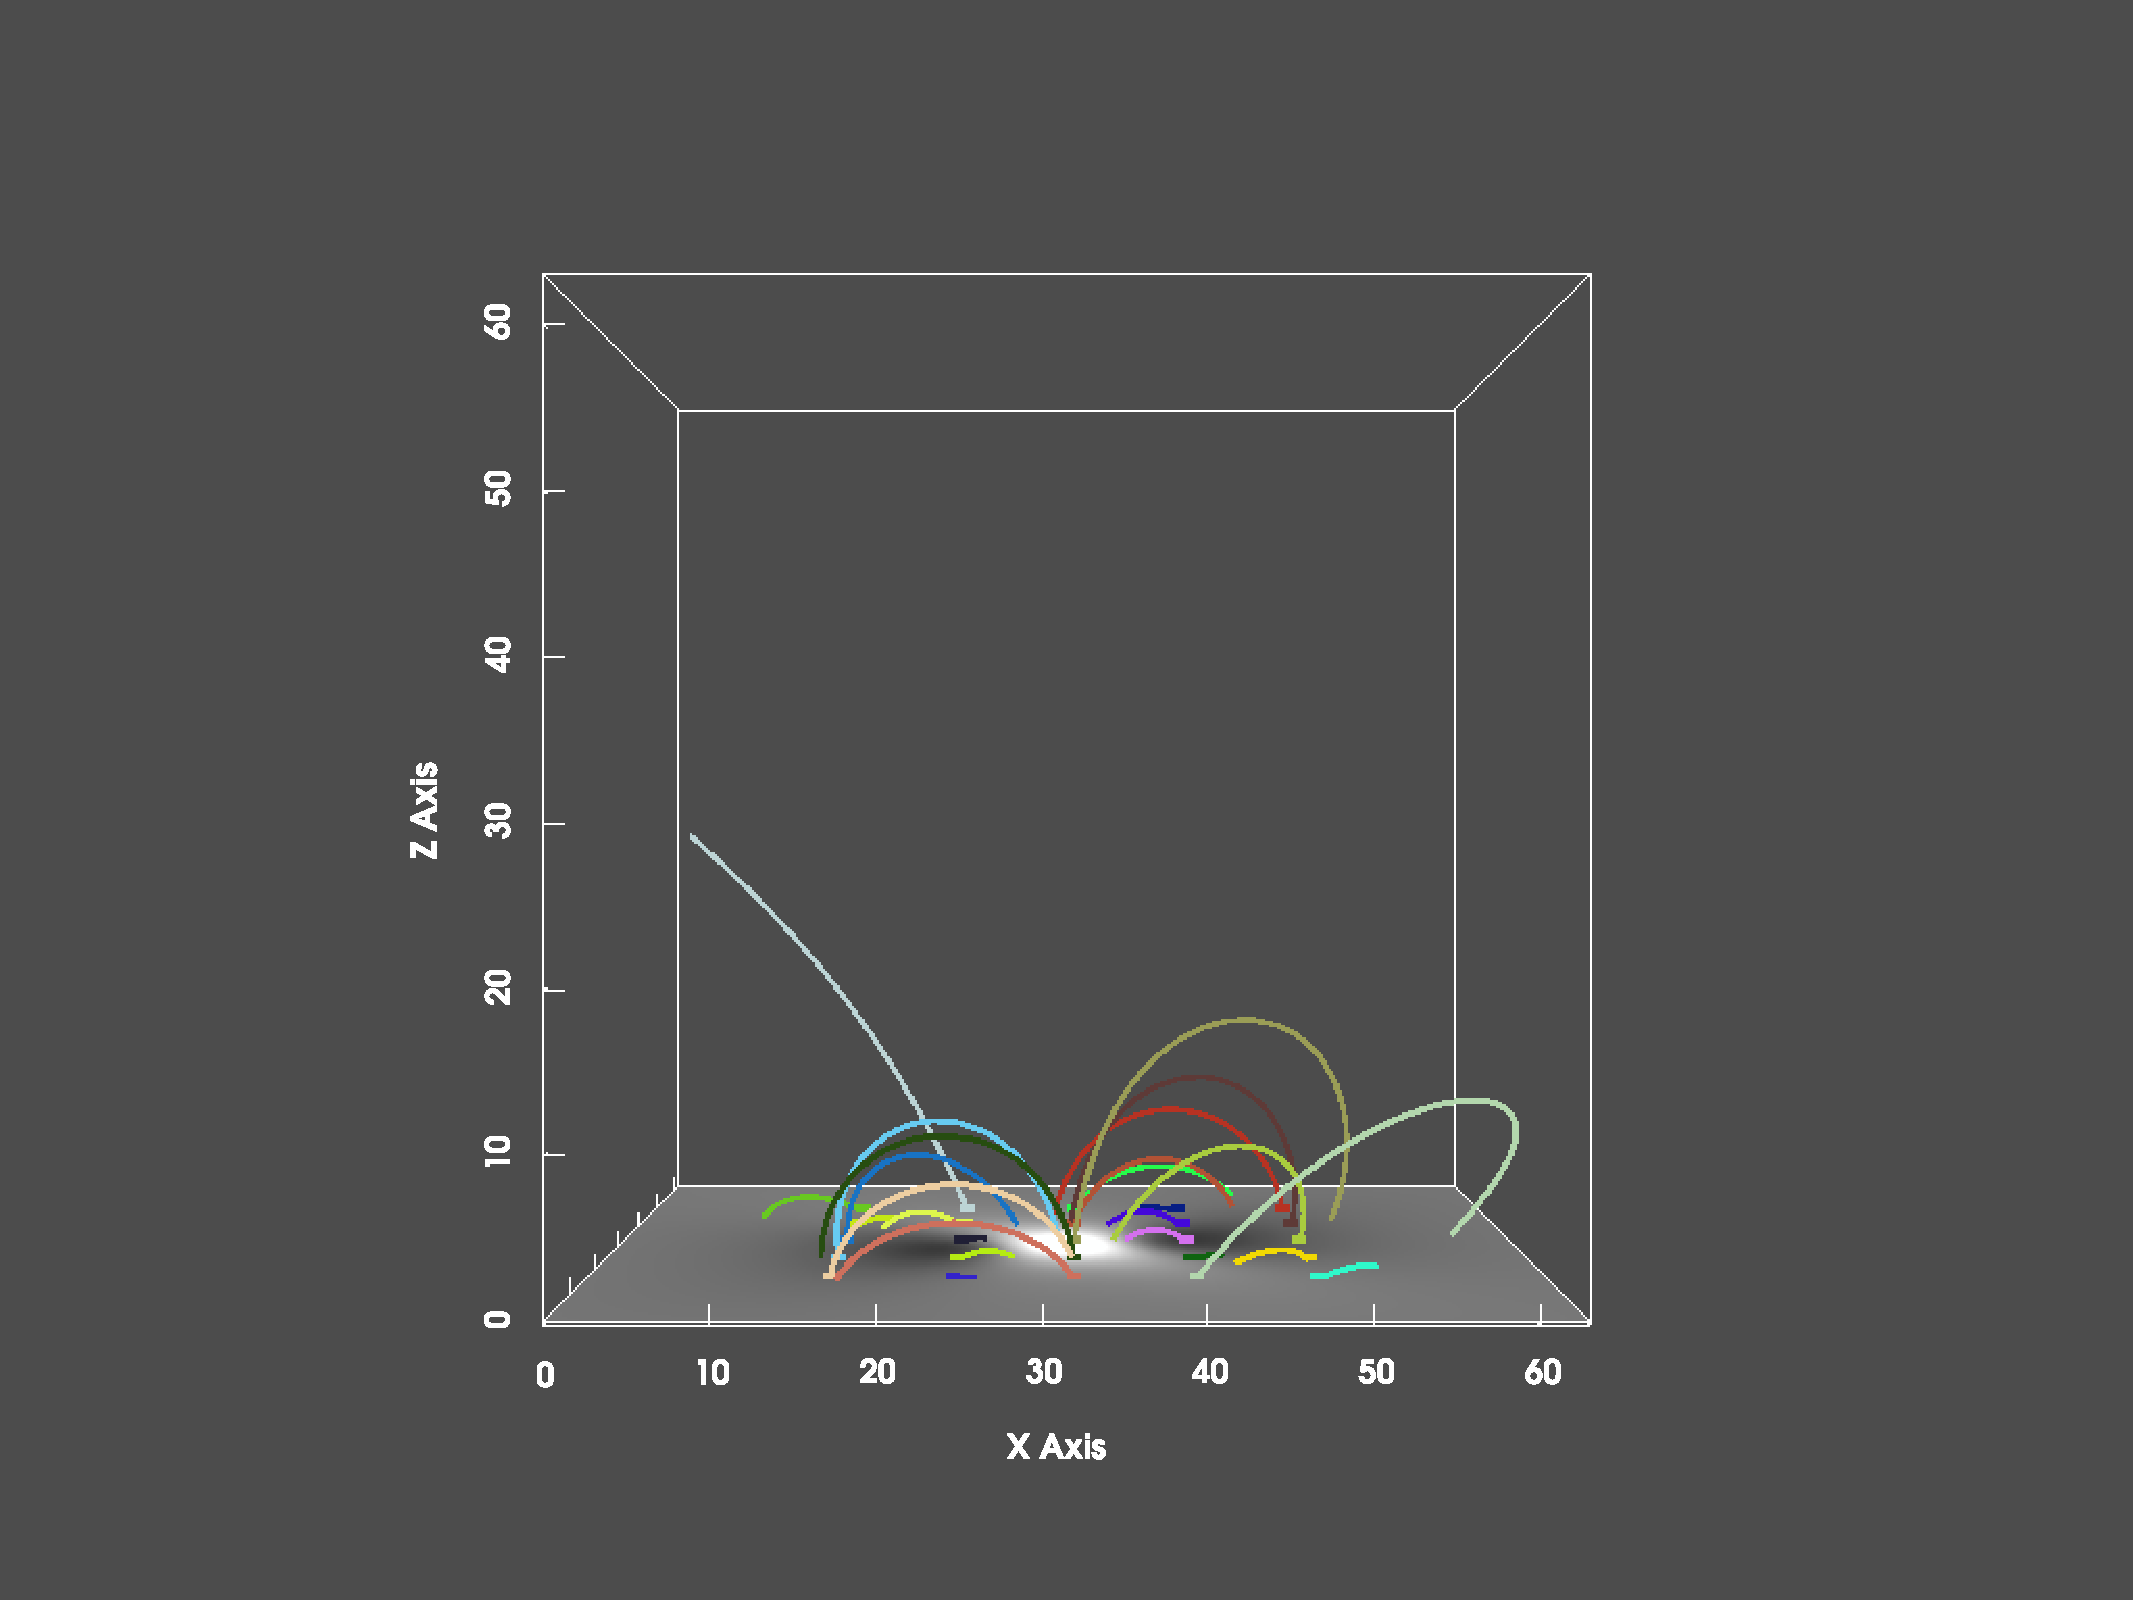
\includegraphics[trim={6cm 1cm 6cm 2cm}, clip, width=\linewidth]{"img/LL_pot_xz.pdf"}
  \end{subfigure}%
  \begin{subfigure}{.5\linewidth}
    \centering
    \caption{Low-Lou}
    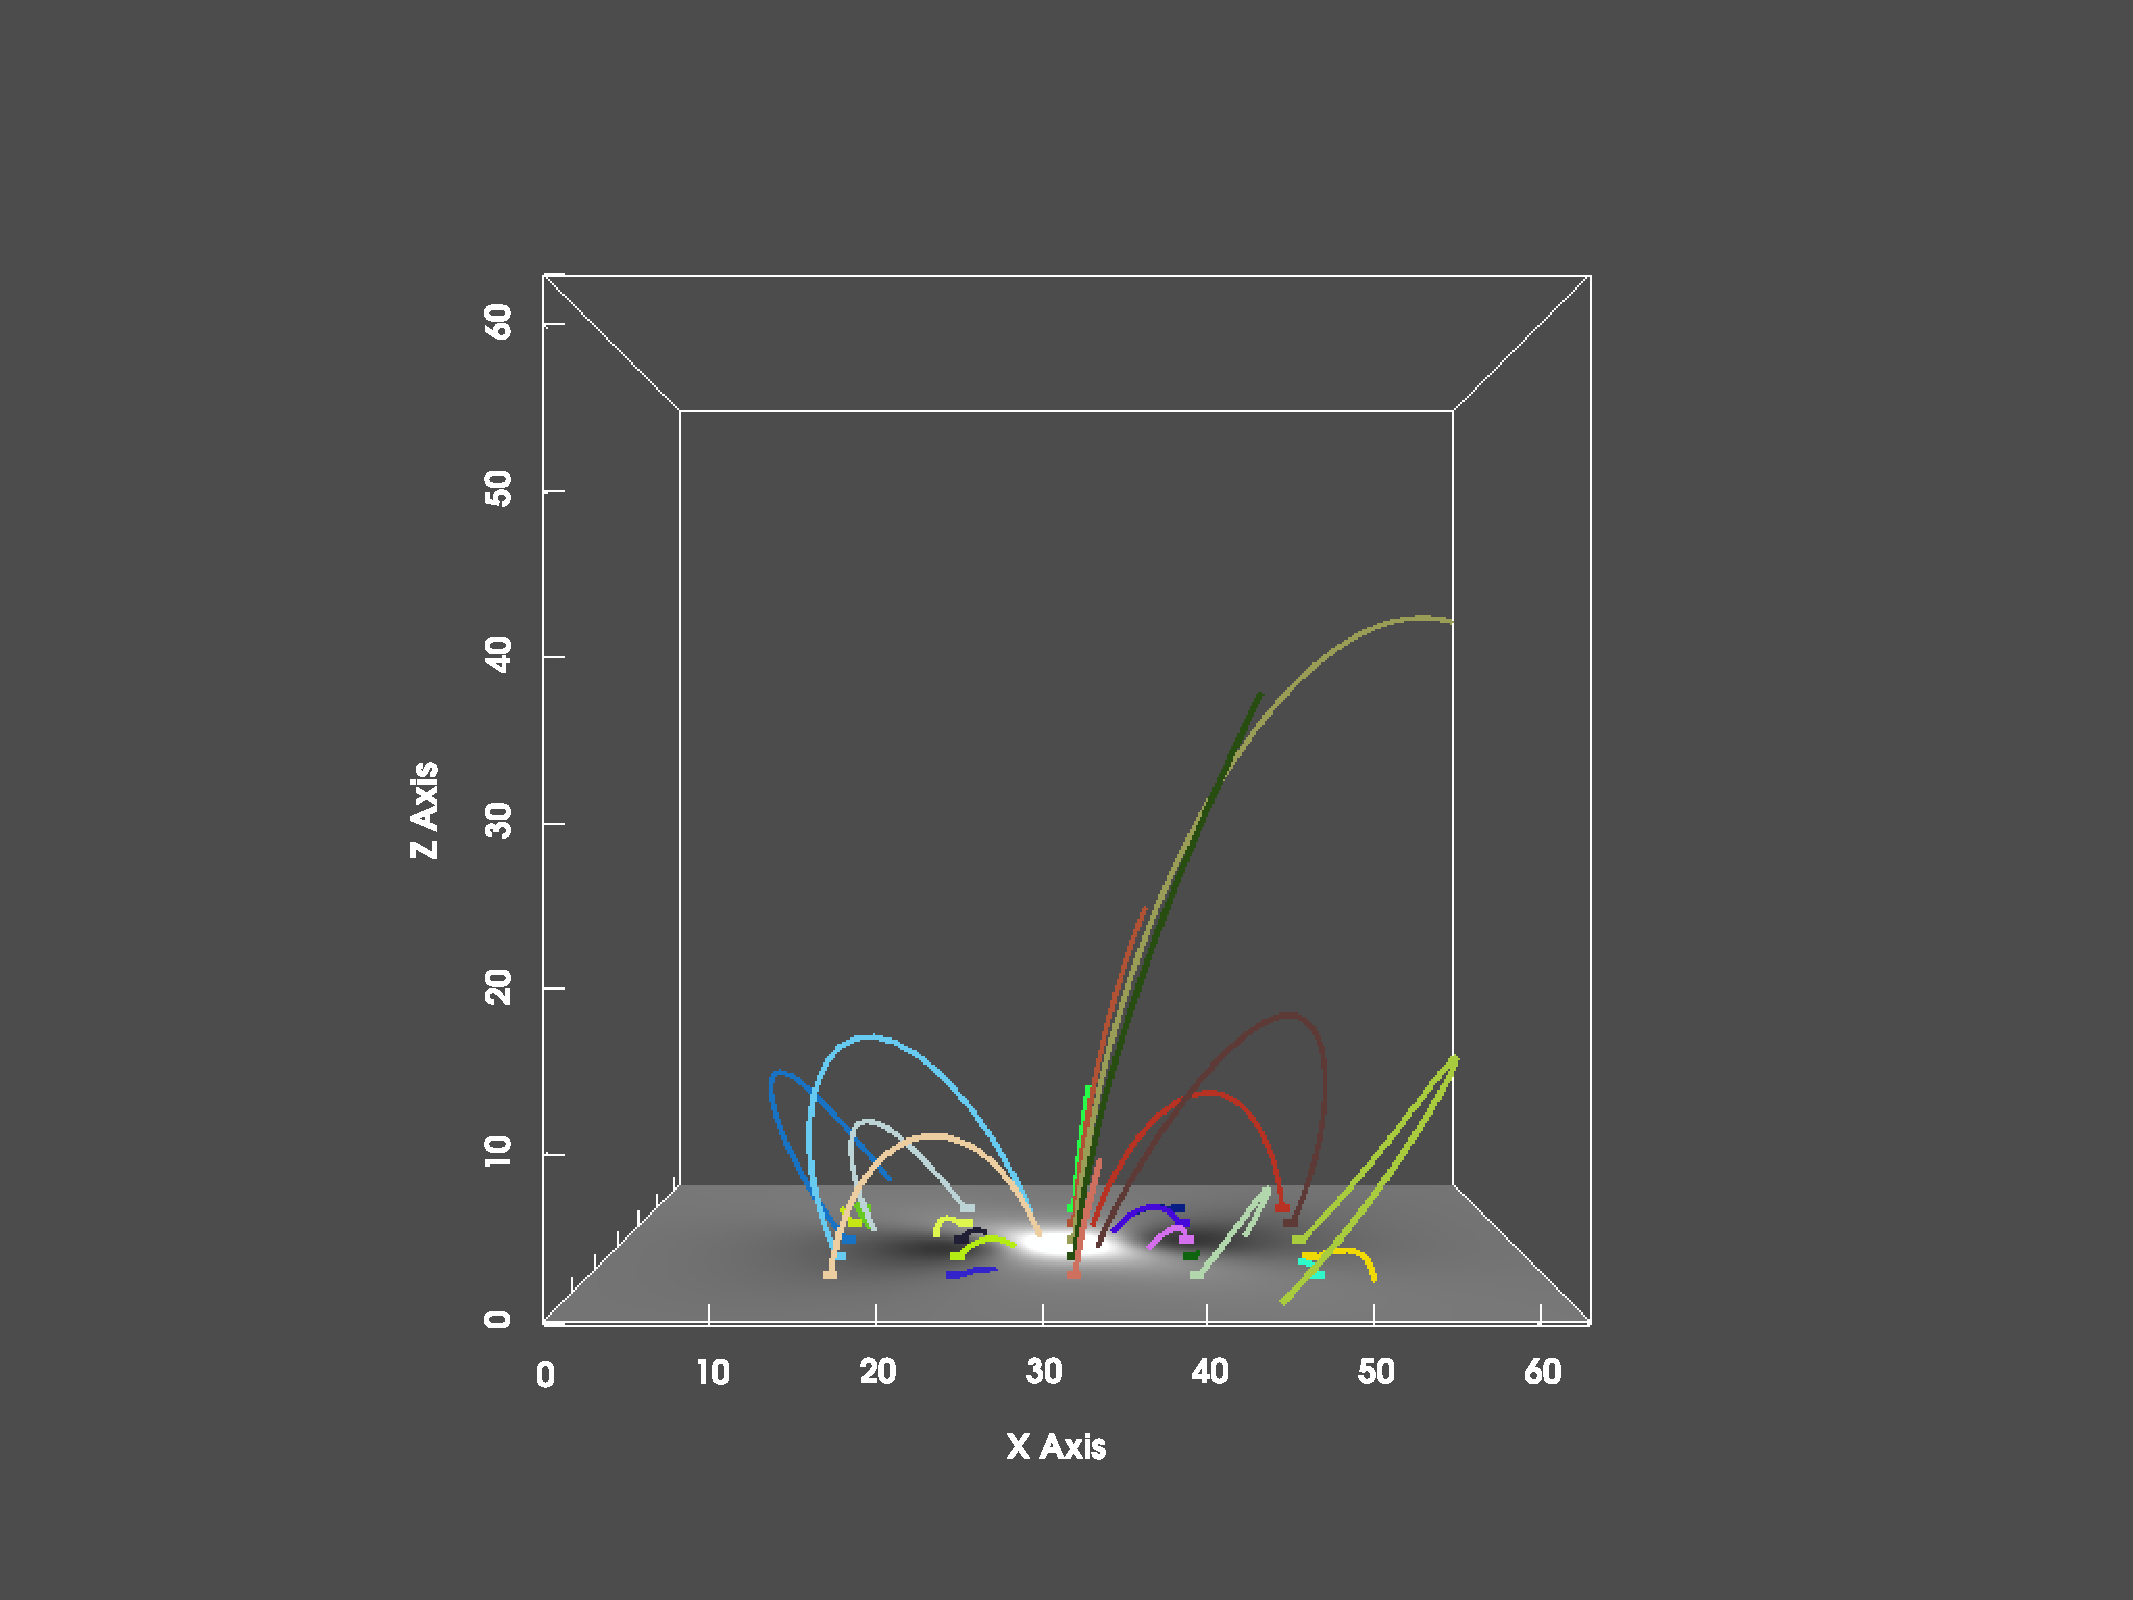
\includegraphics[trim={6cm 1cm 6cm 2cm}, clip, width=\linewidth]{"img/LL_xz.pdf"}
  \end{subfigure}
  
  \caption{The magnetic fields in the xz plane. Each field line is distinguished by its unique color, which is determined by its footpoint at $z=0$ plane.}\label{fig:xz}
\end{figure}


\begin{figure}
  \begin{subfigure}{.5\linewidth}
    \centering
    \caption{PINN(0)}\label{fig:pv0}
    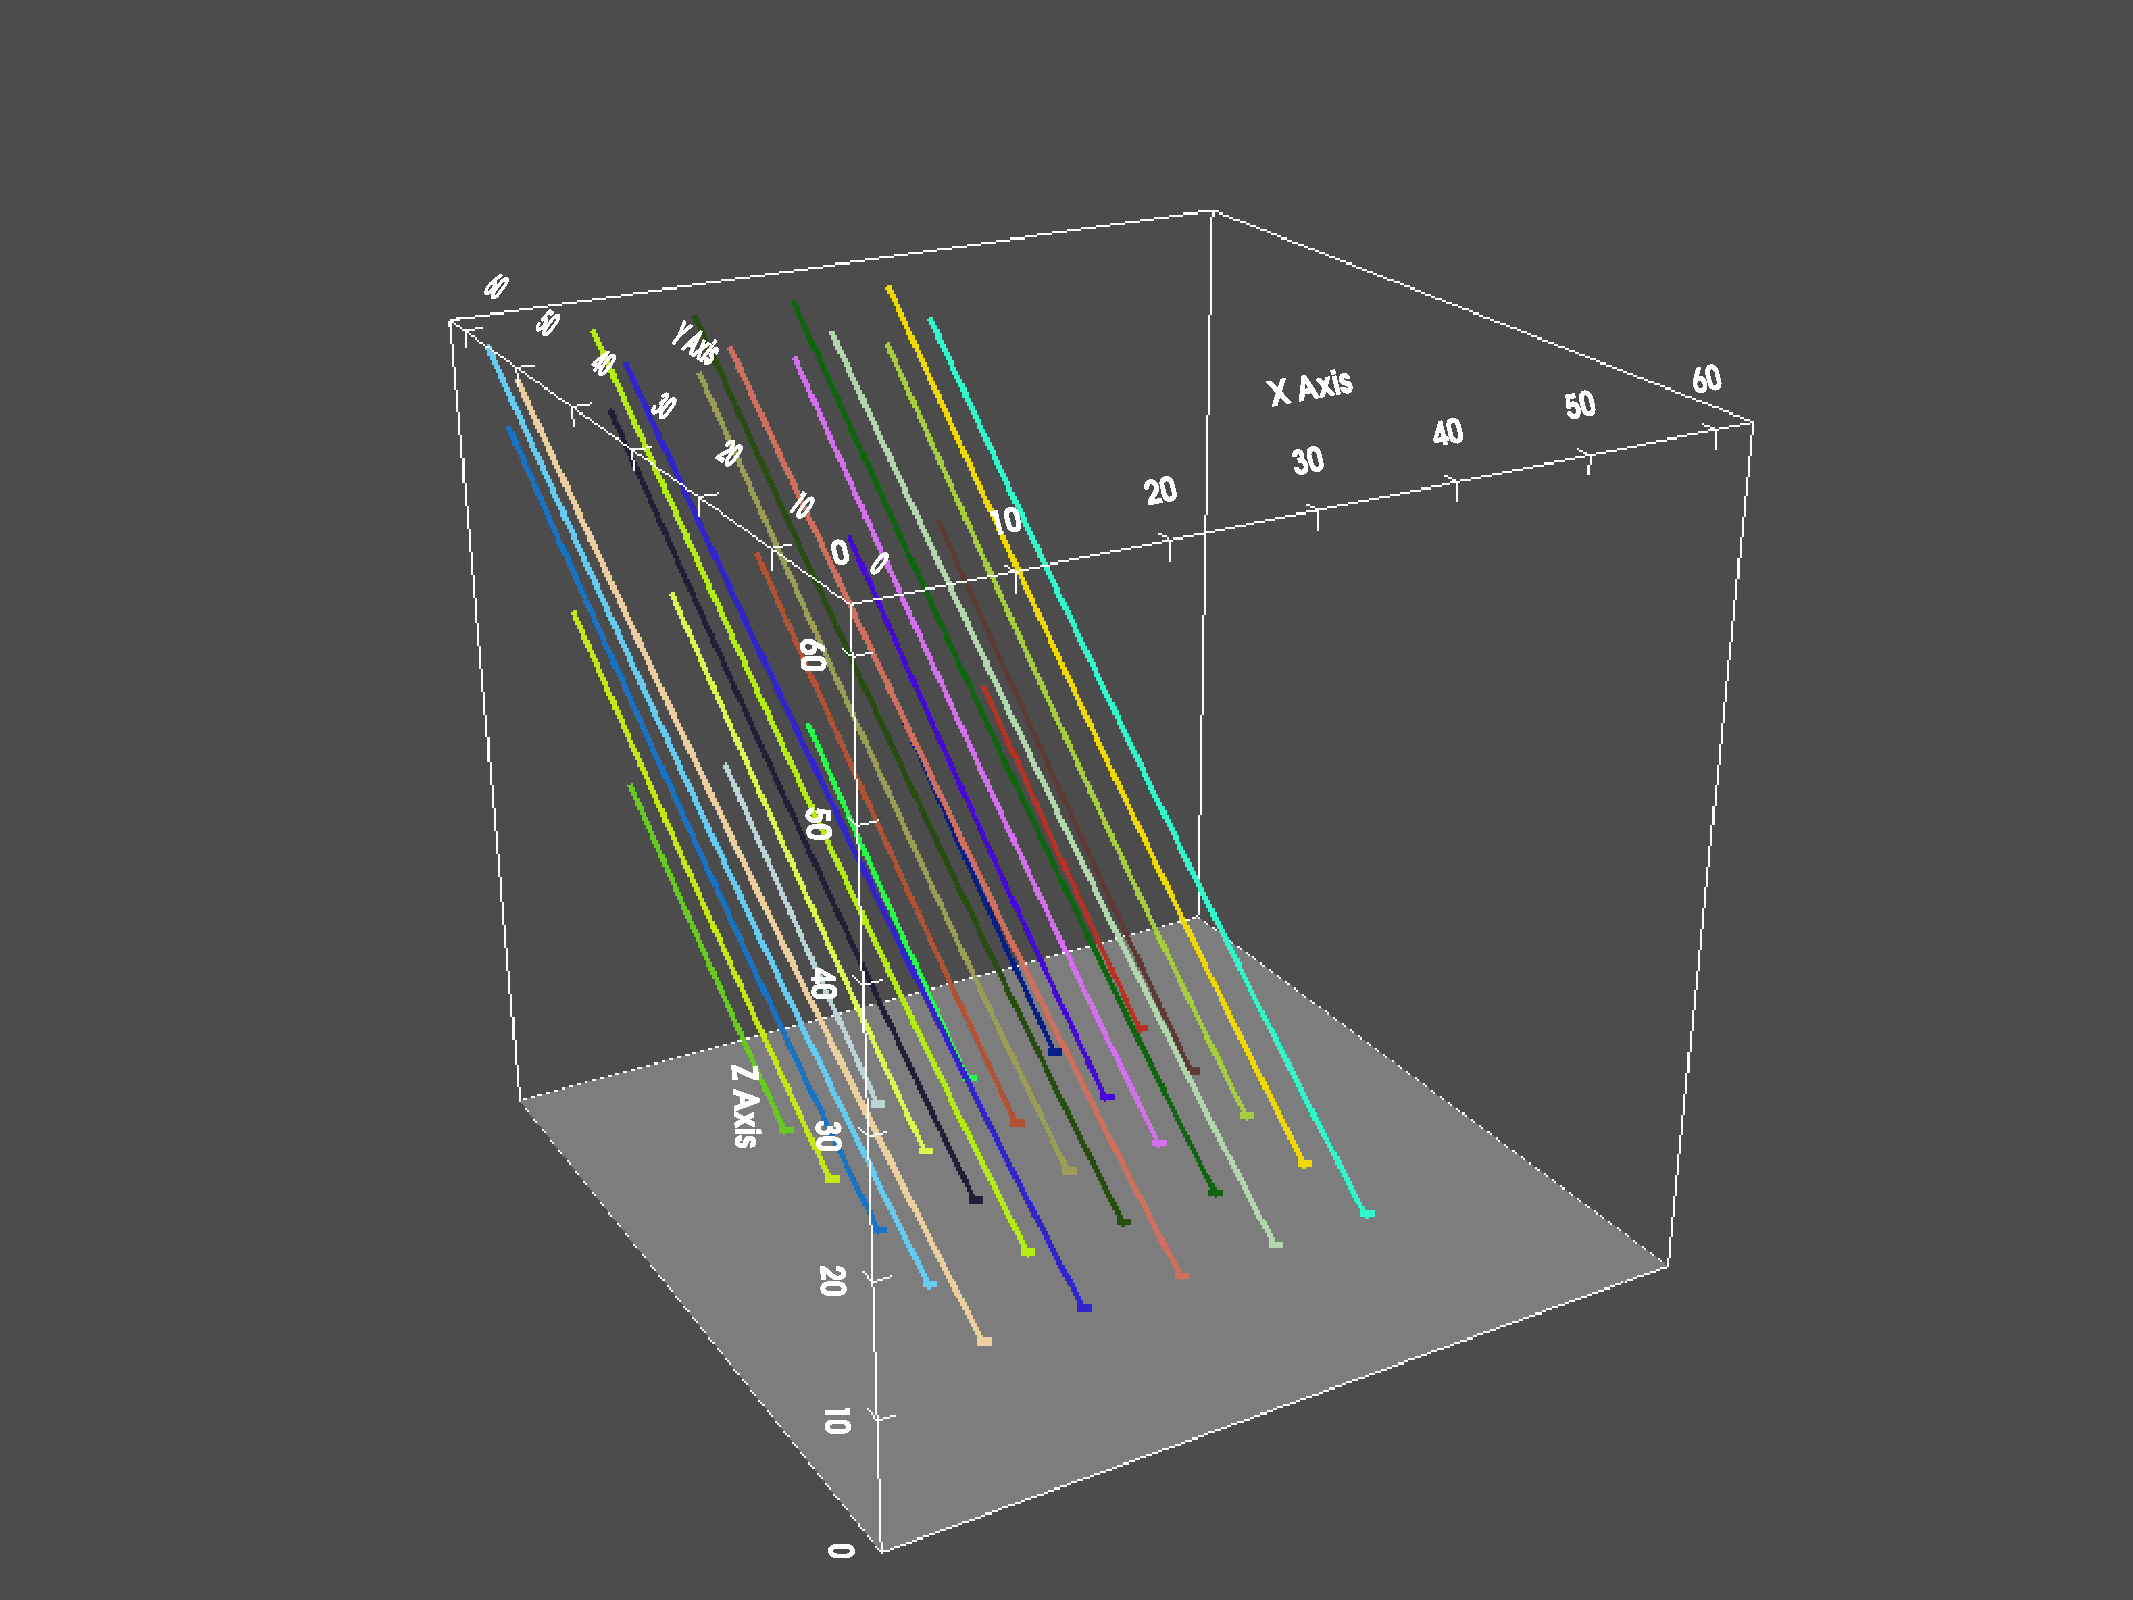
\includegraphics[trim={6cm 0cm 6cm 3cm}, clip, width=\linewidth]{"img/PINN_000000_xz_tilted.pdf"}
  \end{subfigure}%
  \begin{subfigure}{.5\linewidth}
    \centering
    \caption{PINN(100)}
    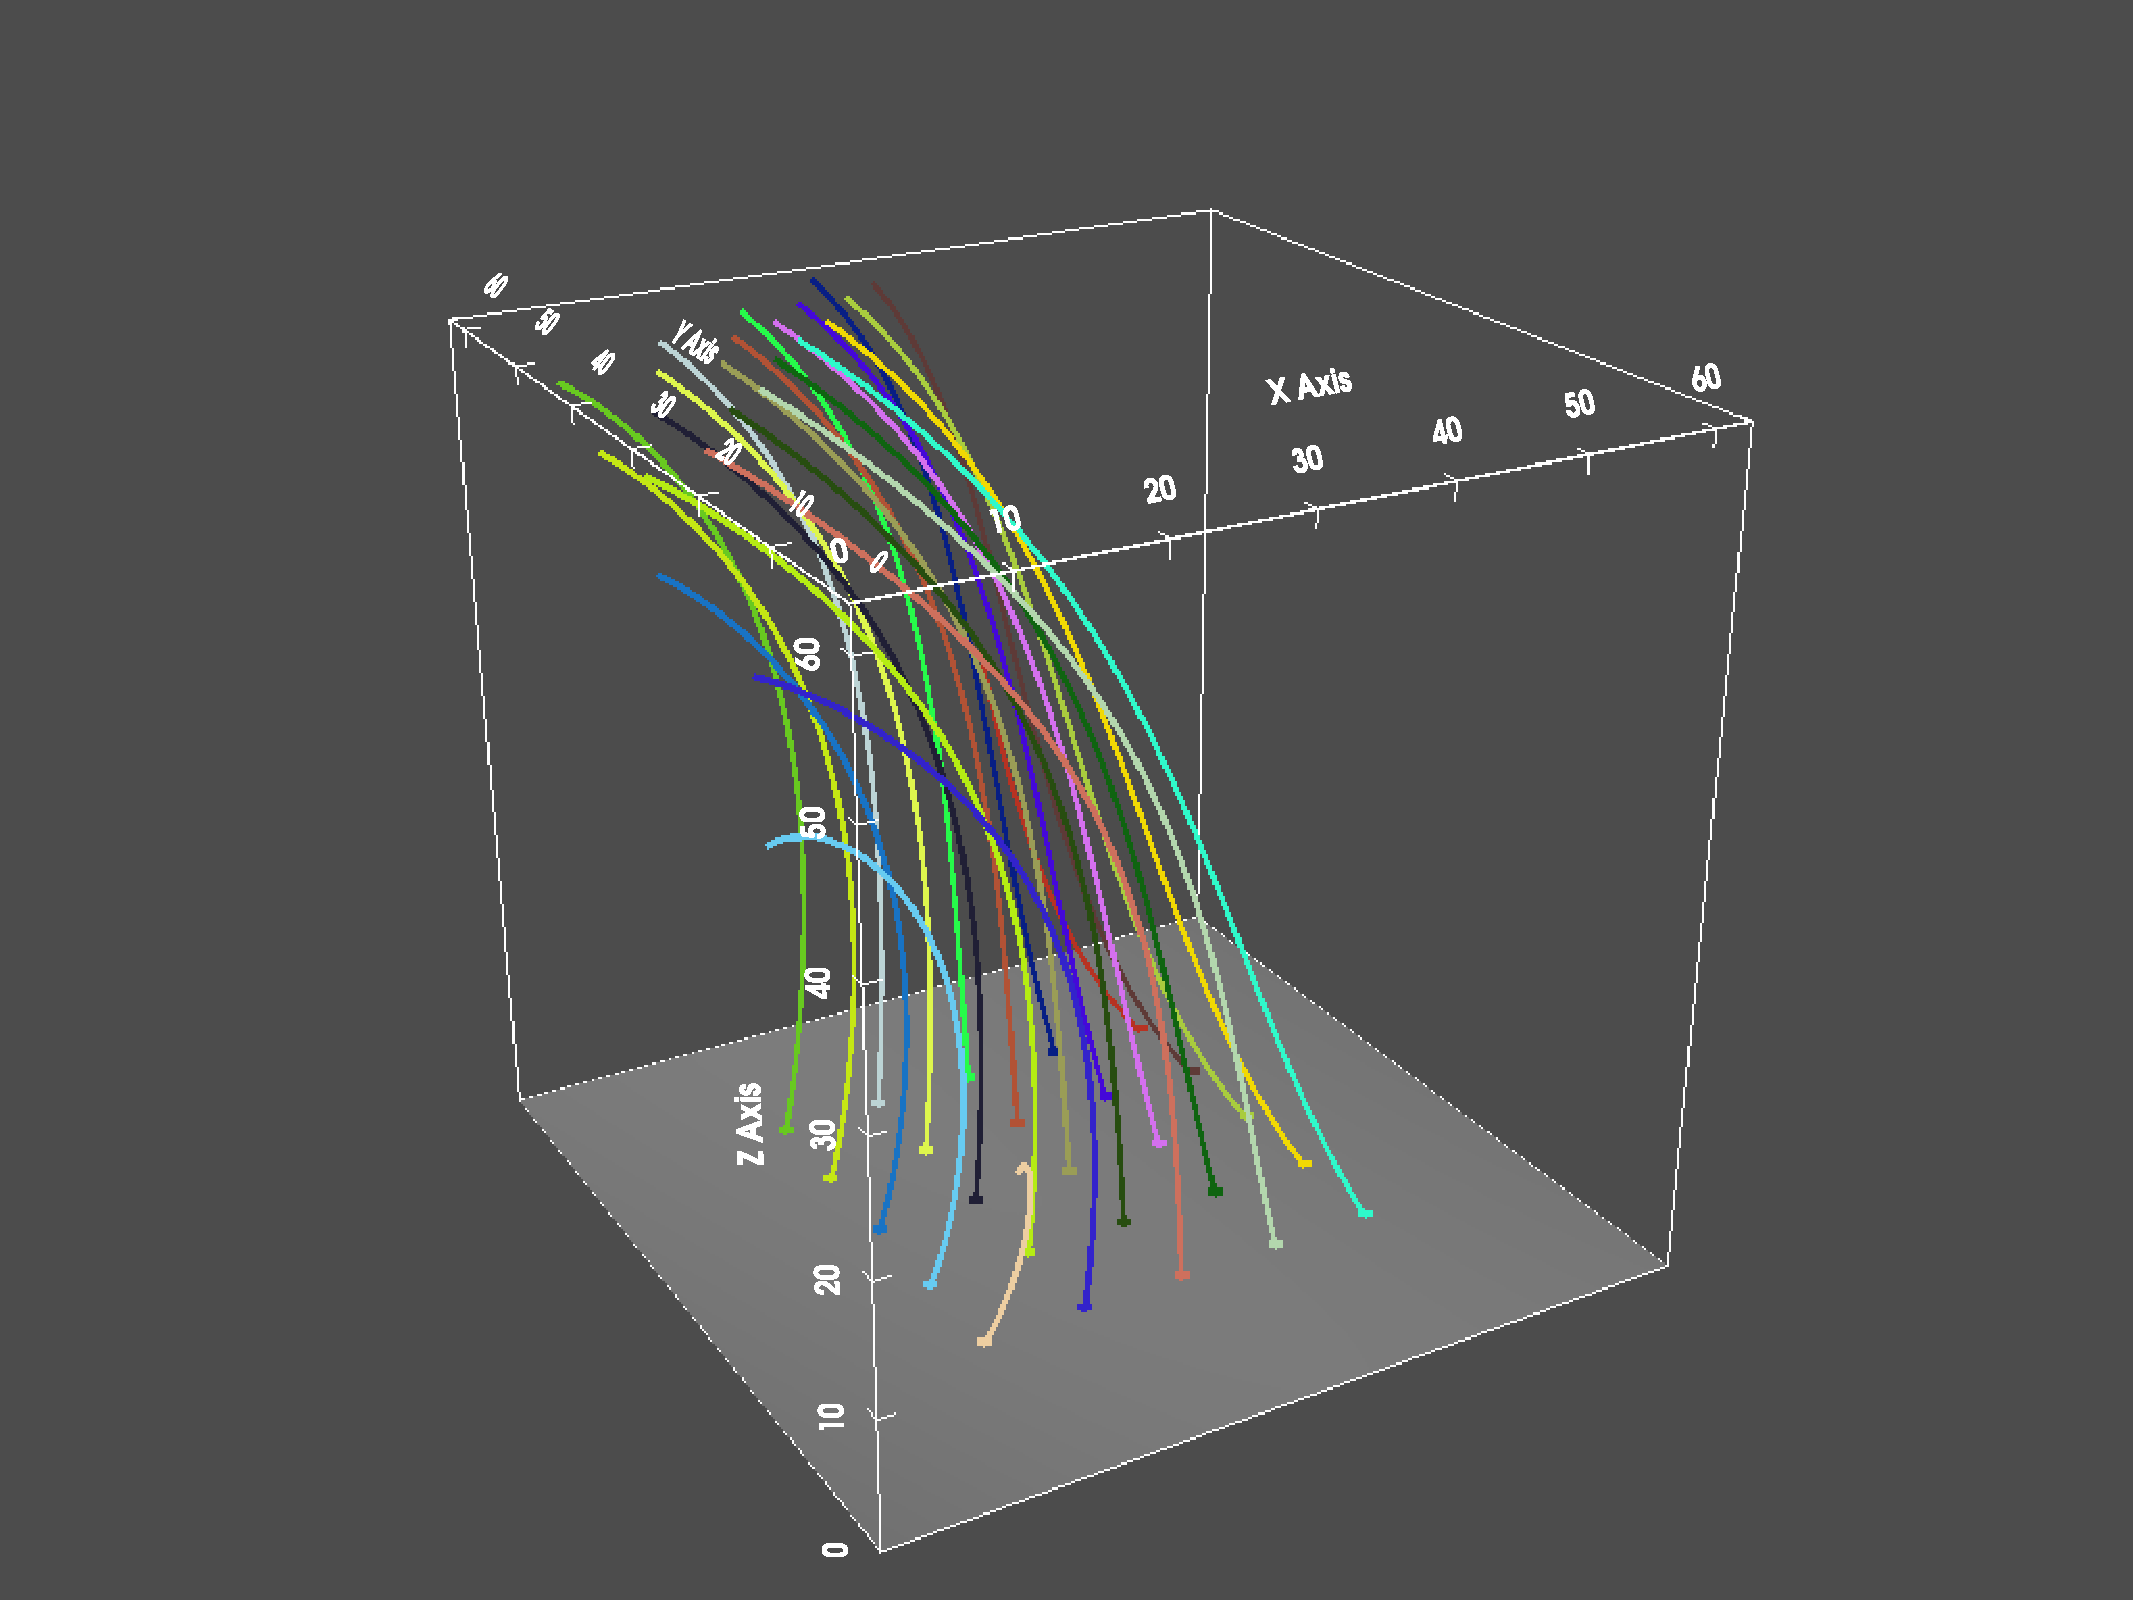
\includegraphics[trim={6cm 0cm 6cm 3cm}, clip, width=\linewidth]{"img/PINN_000100_xz_tilted.pdf"}
  \end{subfigure}

  \begin{subfigure}{.5\linewidth}
    \centering
    \caption{PINN(1000)}
    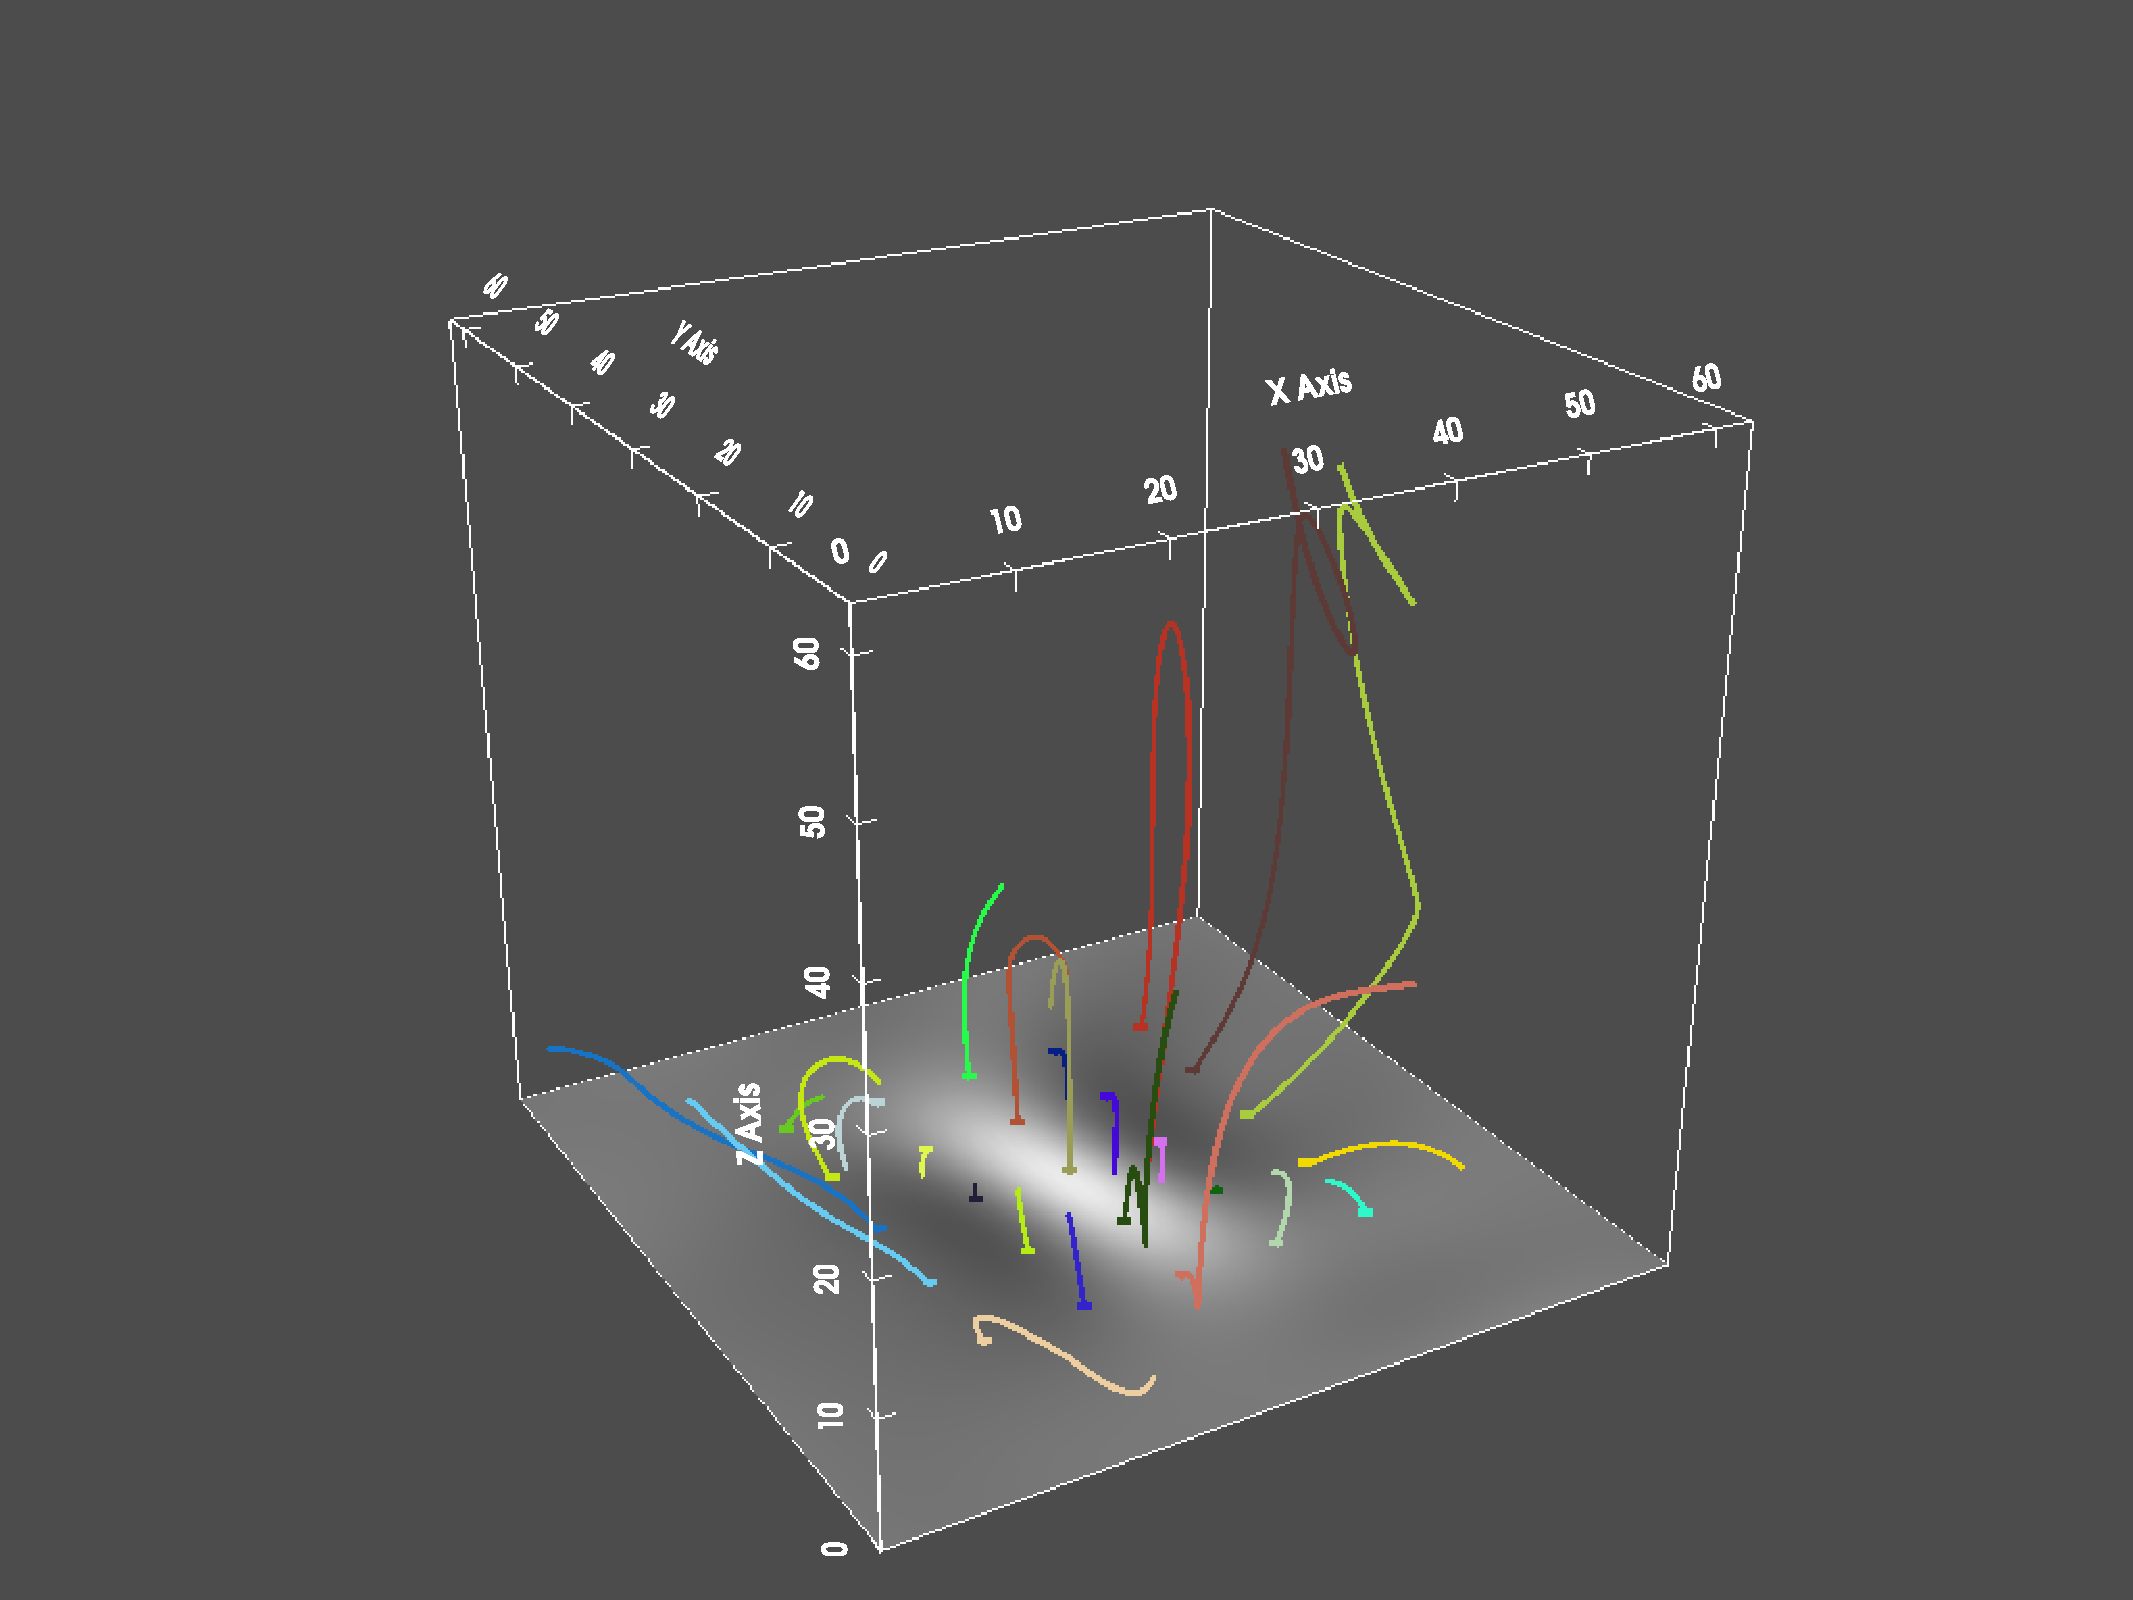
\includegraphics[trim={6cm 0cm 6cm 3cm}, clip, width=\linewidth]{"img/PINN_001000_xz_tilted.pdf"}
  \end{subfigure}%
  \begin{subfigure}{.5\linewidth}
    \centering
    \caption{PINN(10000)}
    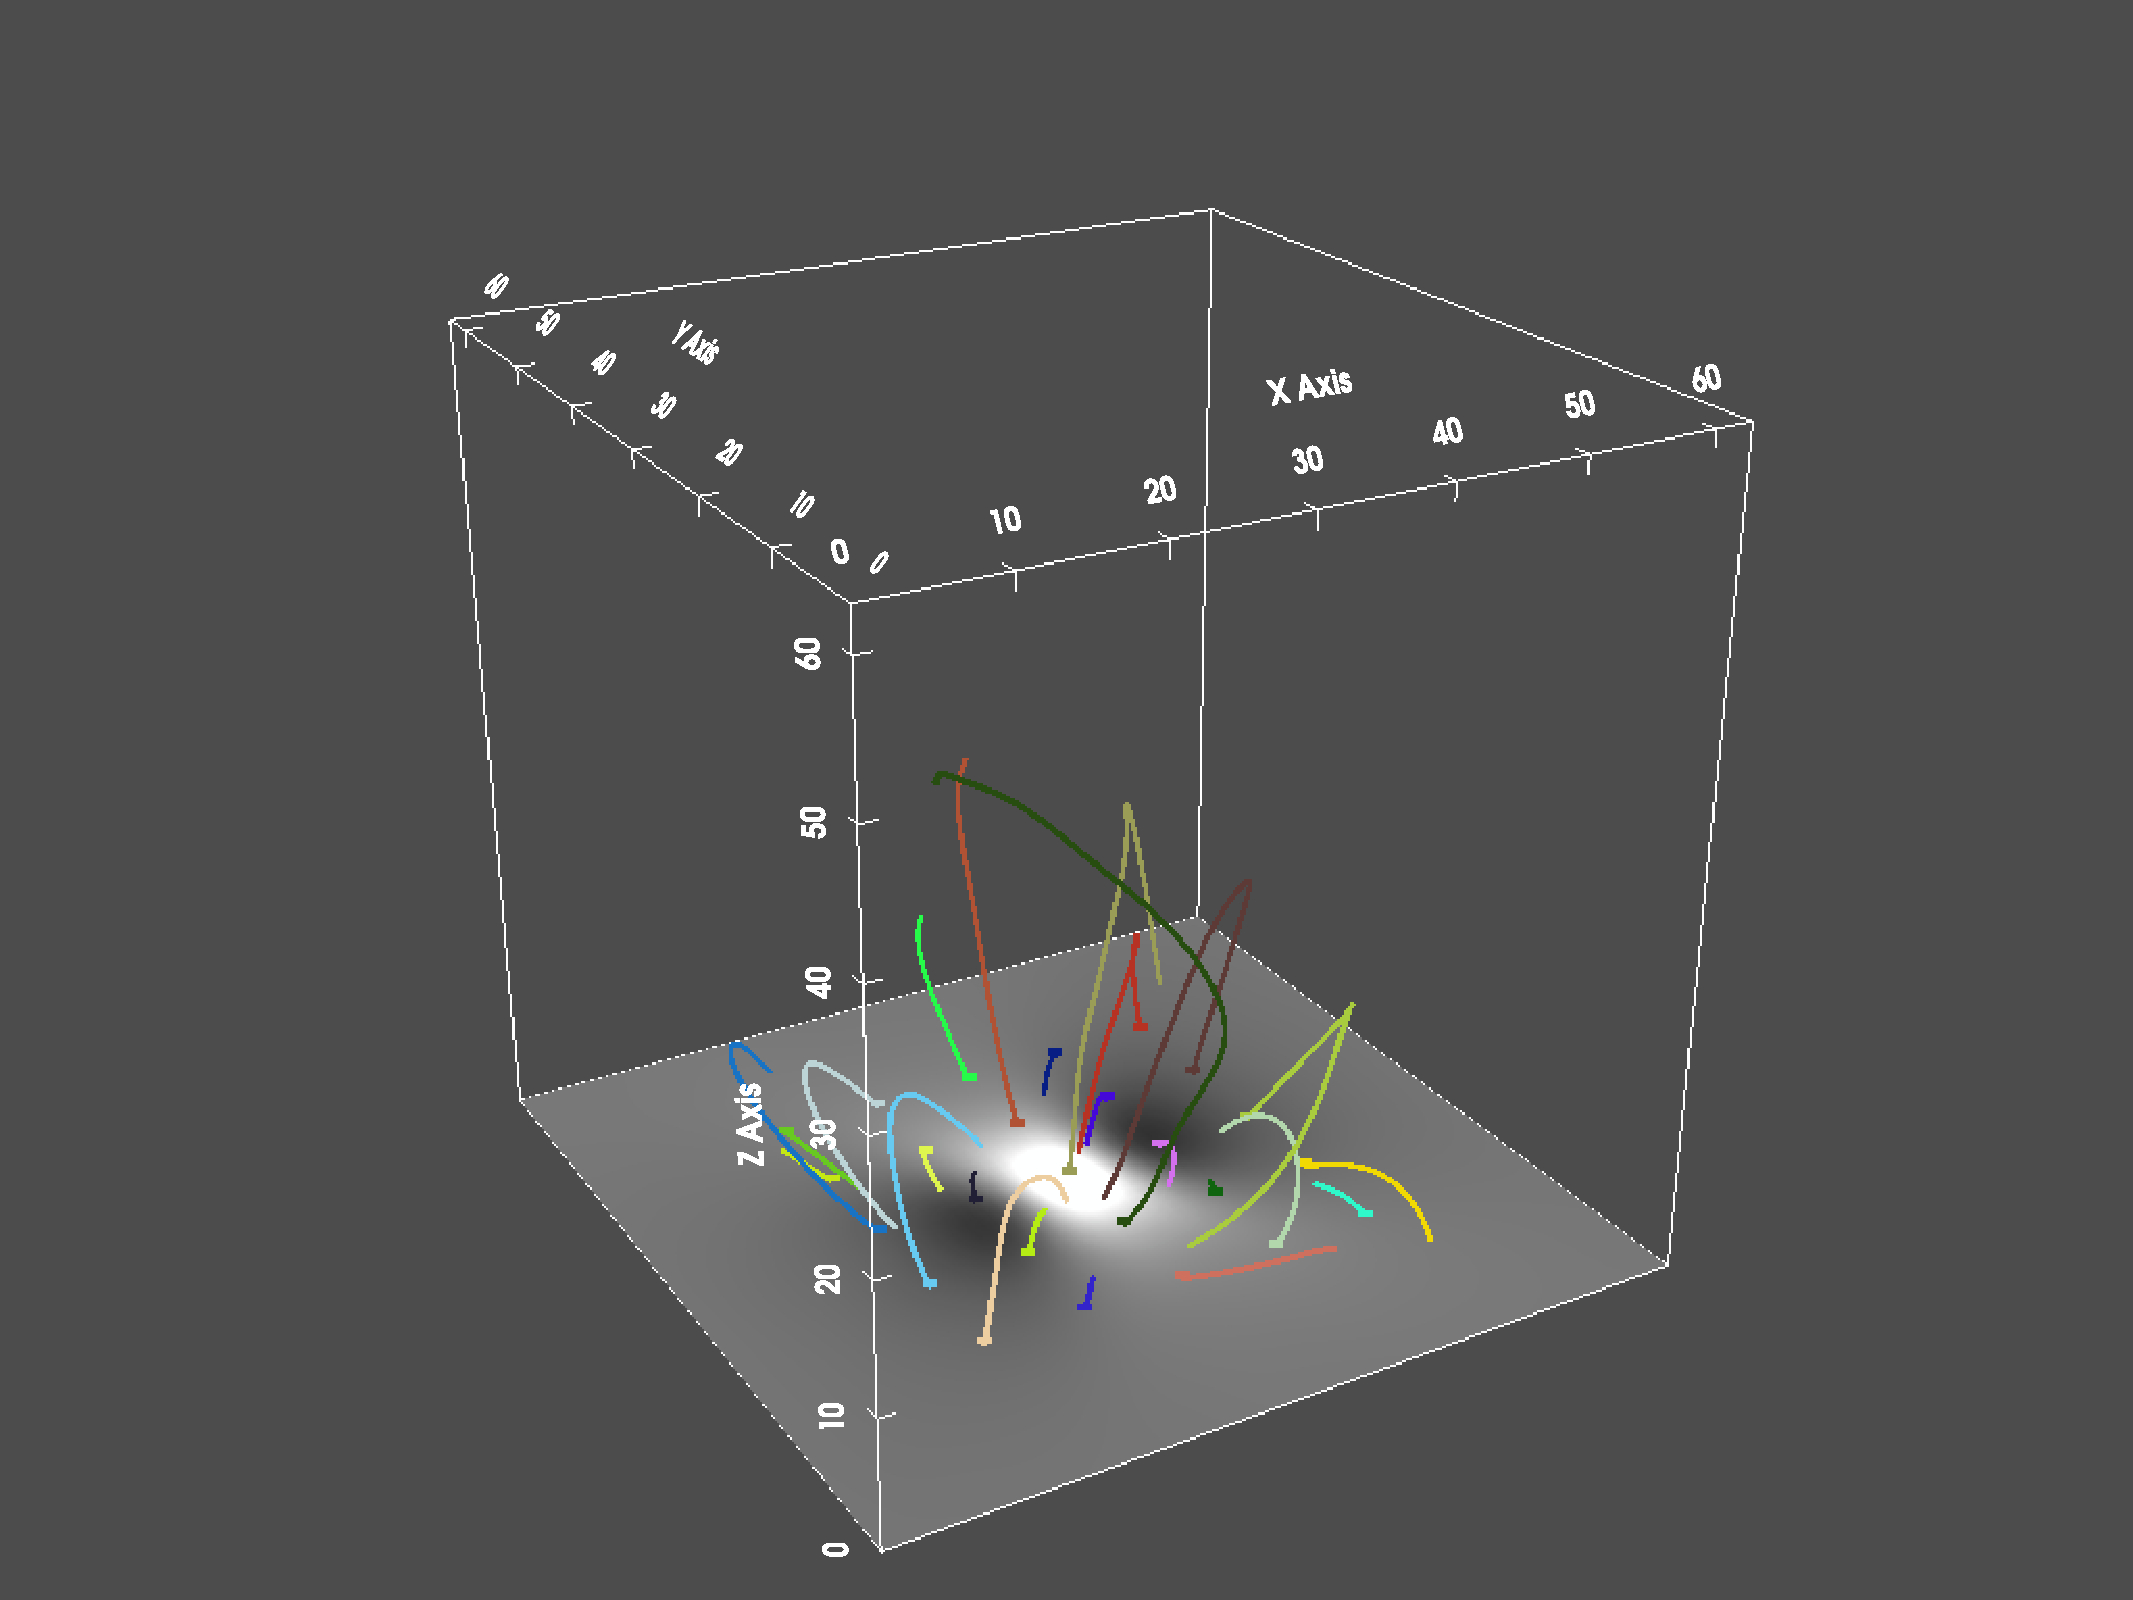
\includegraphics[trim={6cm 0cm 6cm 3cm}, clip, width=\linewidth]{"img/PINN_010000_xz_tilted.pdf"}
  \end{subfigure}

  \begin{subfigure}{.5\linewidth}
    \centering
    \caption{PINN(25000)}
    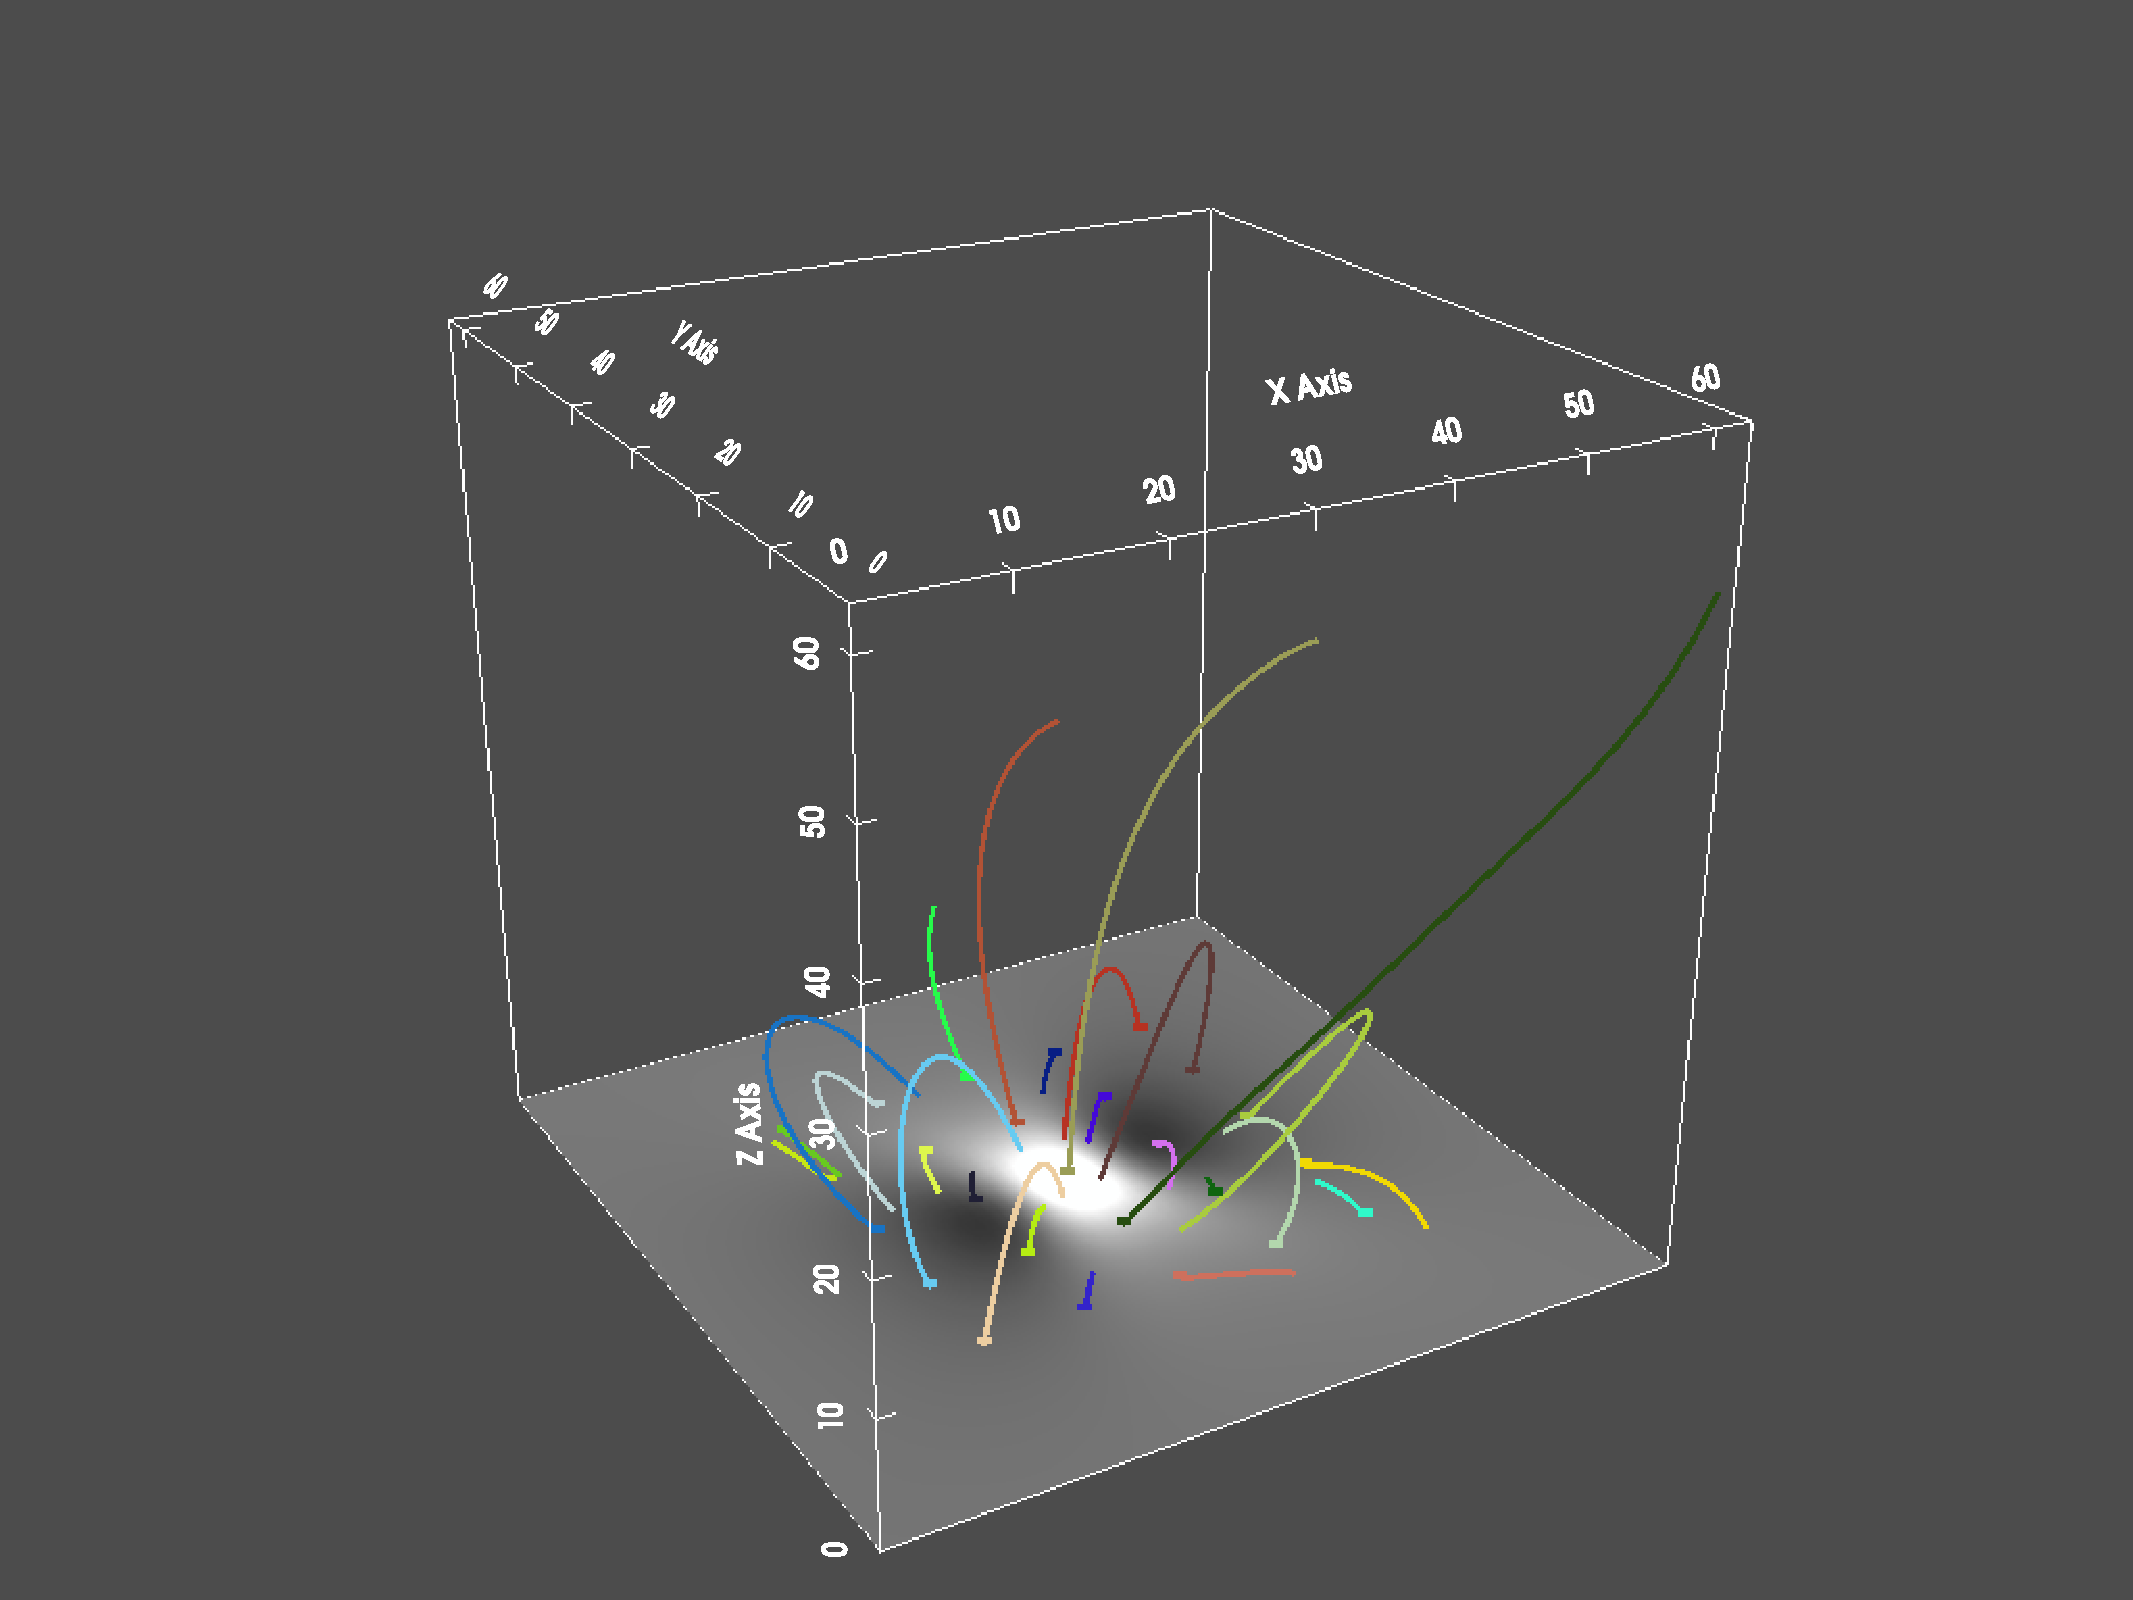
\includegraphics[trim={6cm 0cm 6cm 3cm}, clip, width=\linewidth]{"img/PINN_025000_xz_tilted.pdf"}
  \end{subfigure}%
  \begin{subfigure}{.5\linewidth}
    \centering
    \caption{PINN(50000)}
    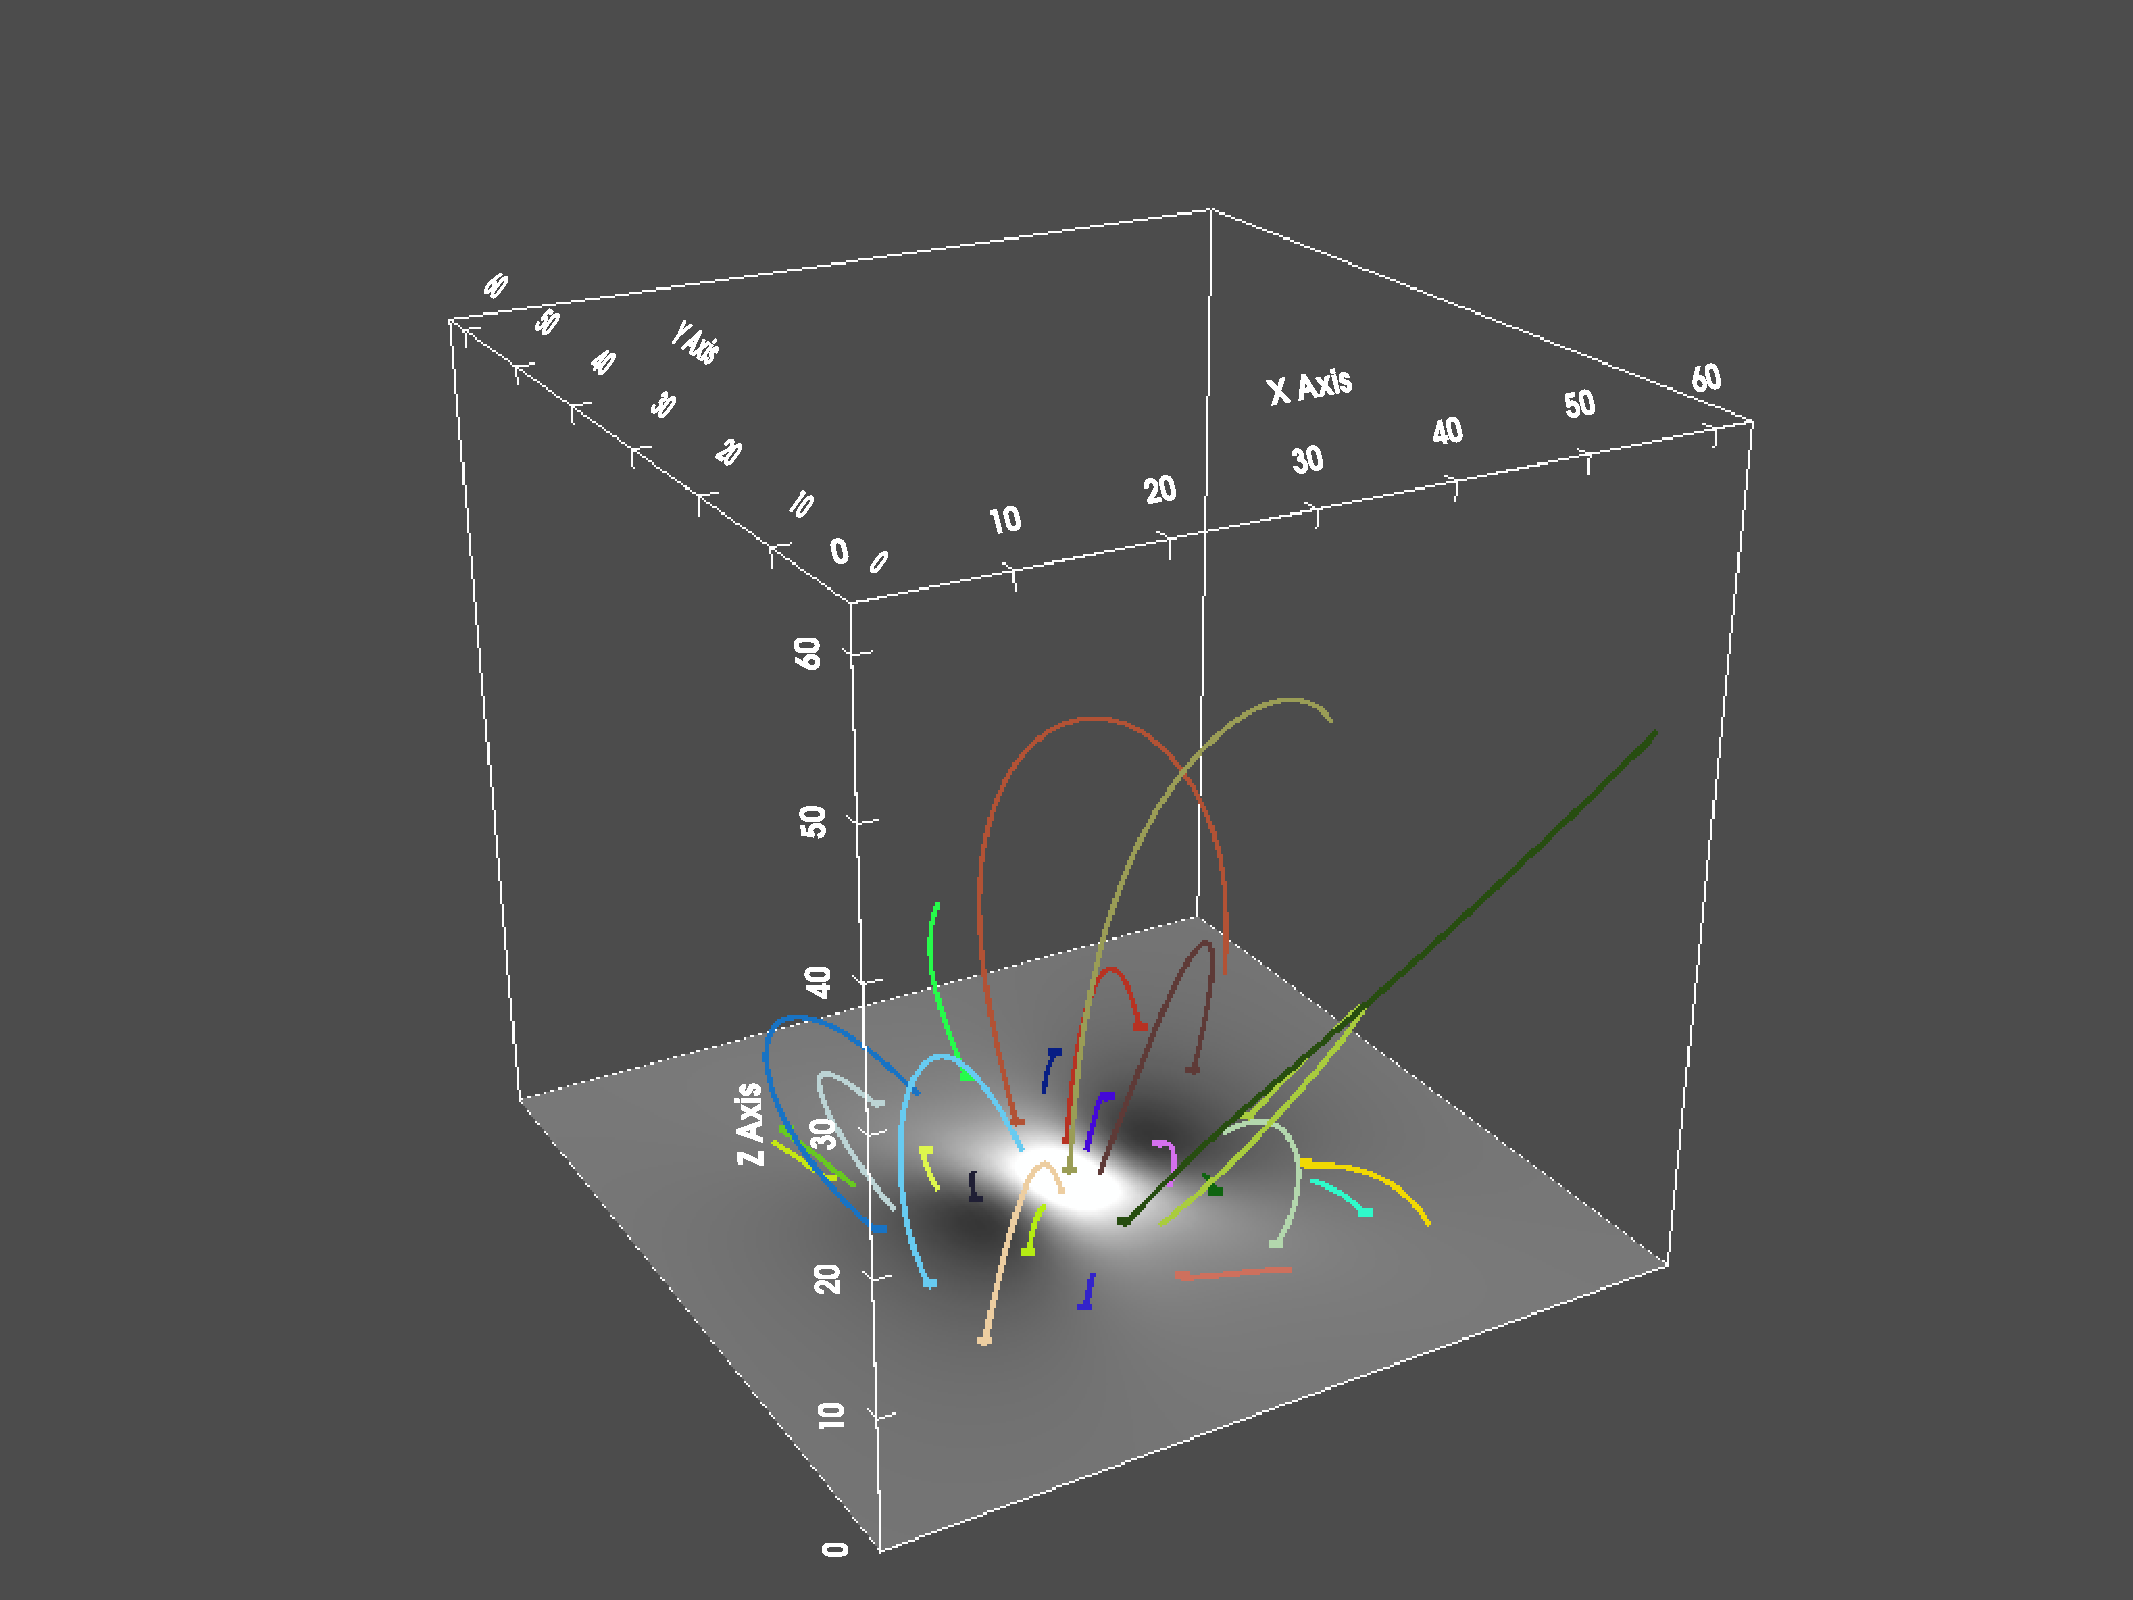
\includegraphics[trim={6cm 0cm 6cm 3cm}, clip, width=\linewidth]{"img/PINN_050000_xz_tilted.pdf"}
  \end{subfigure}
  
  \begin{subfigure}{.5\linewidth}
    \centering
    \caption{Potential}
    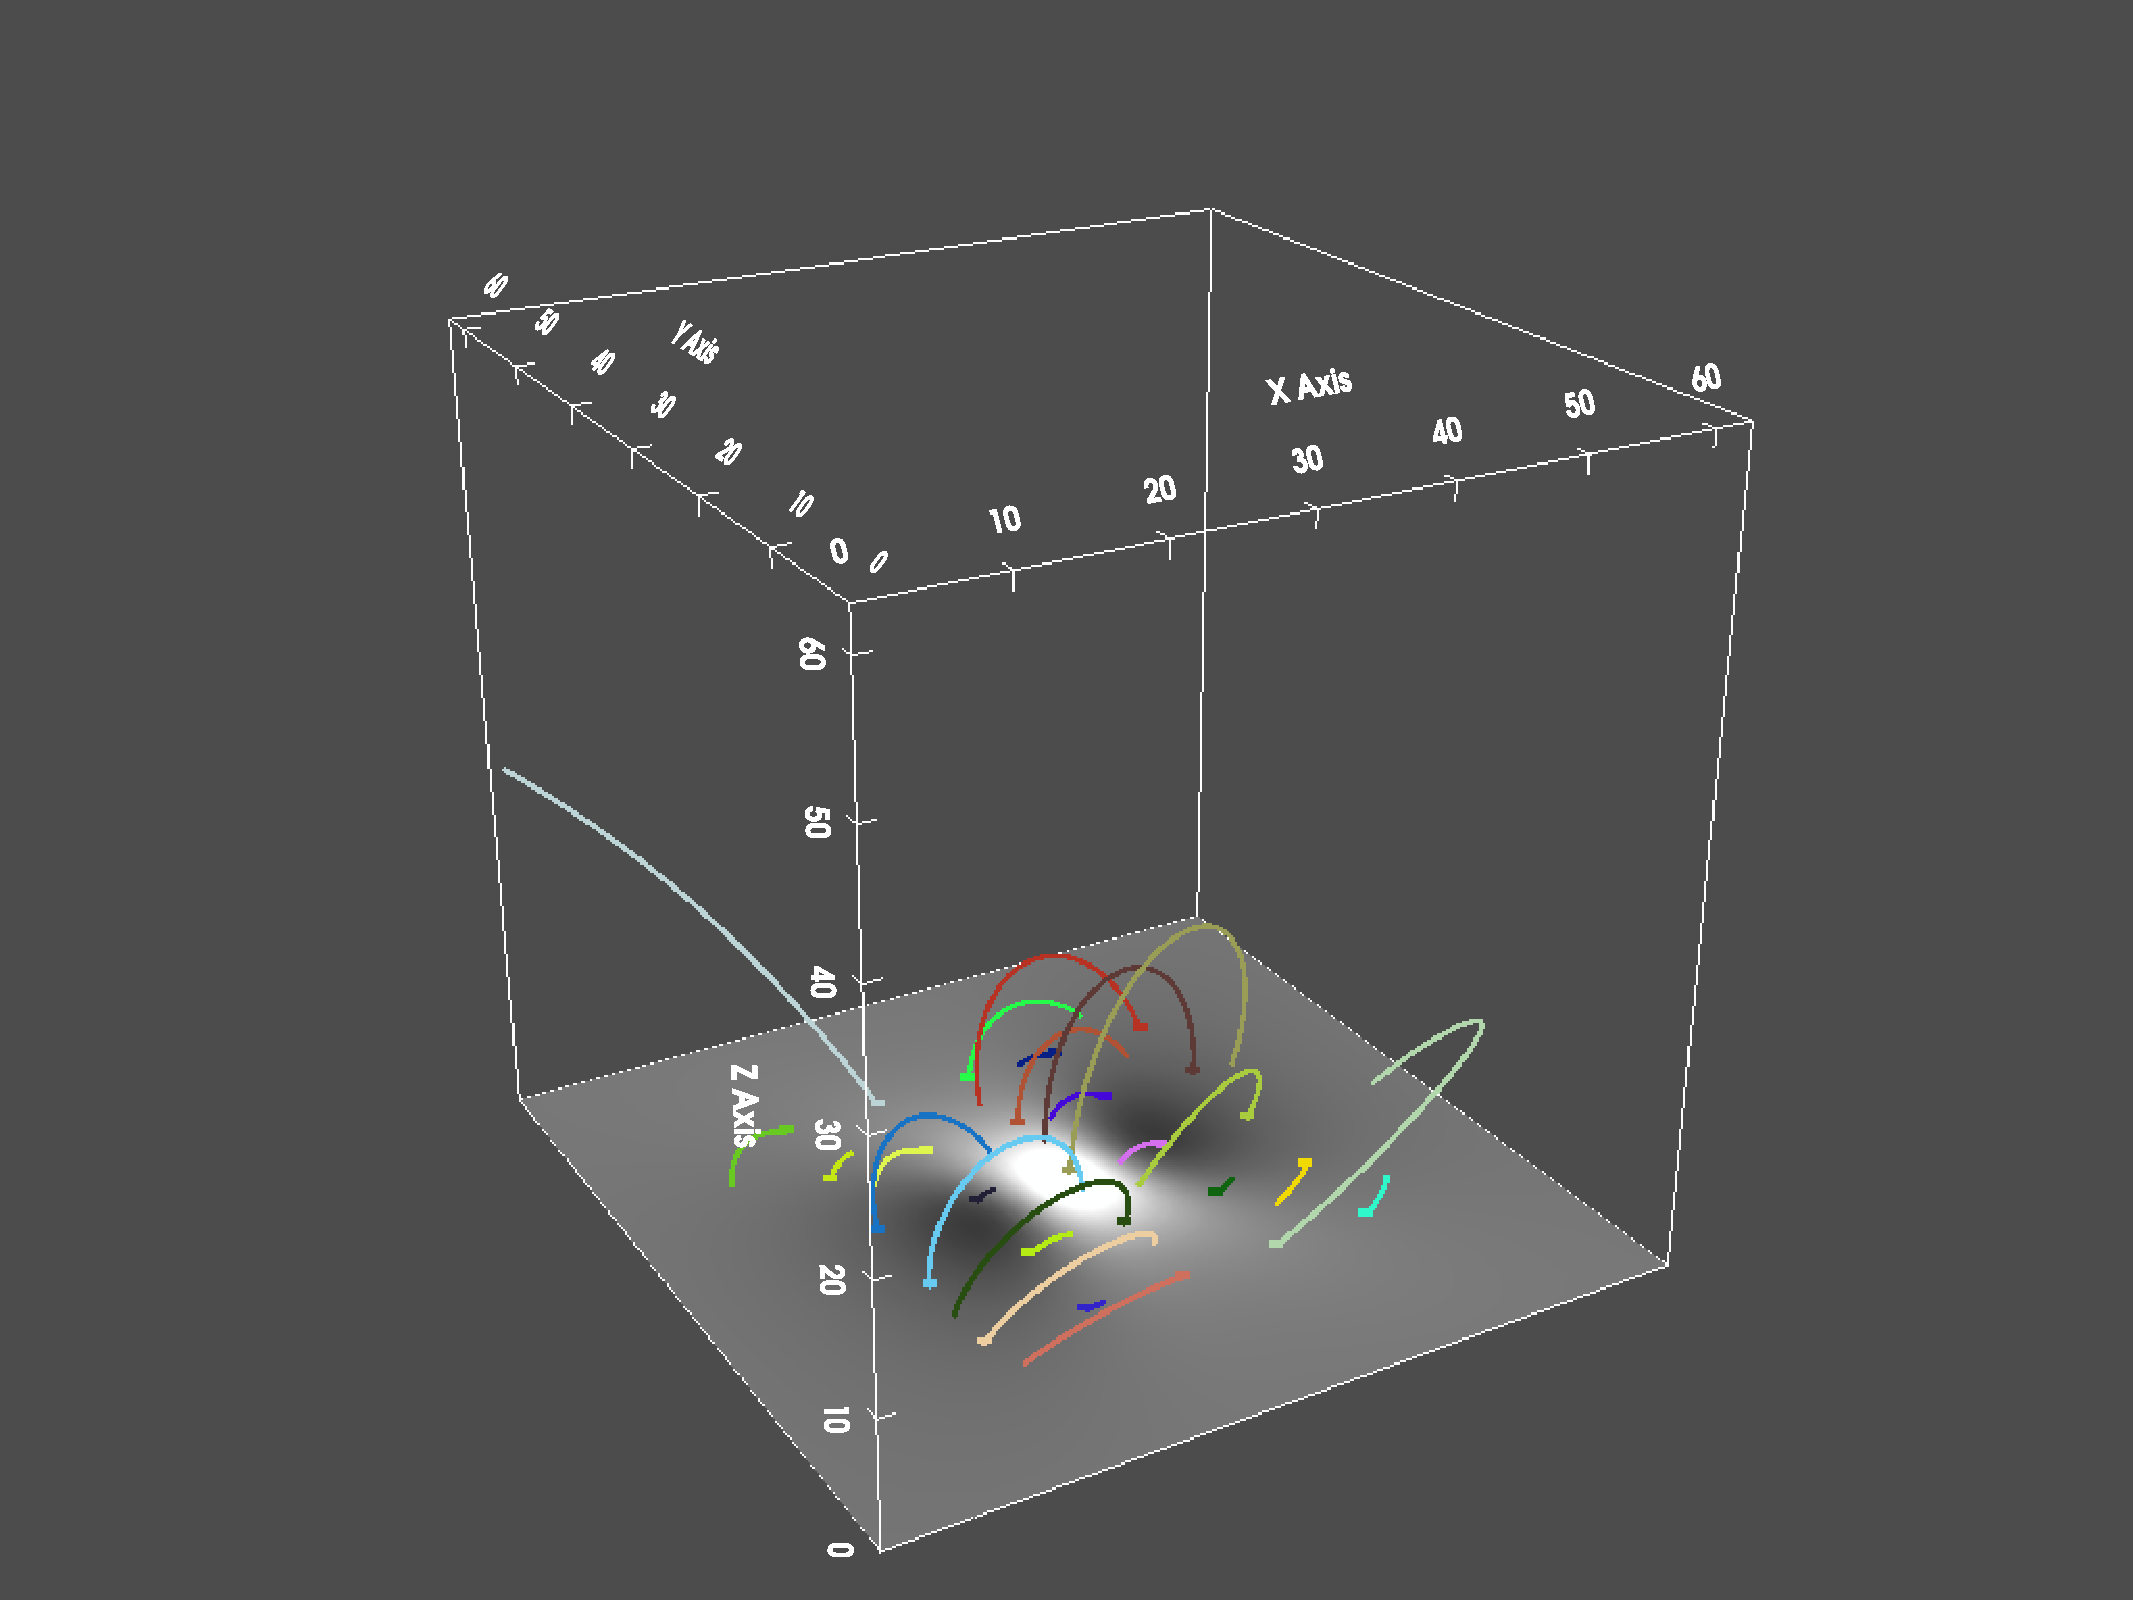
\includegraphics[trim={6cm 0cm 6cm 3cm}, clip, width=\linewidth]{"img/LL_pot_xz_tilted.pdf"}
  \end{subfigure}%
  \begin{subfigure}{.5\linewidth}
    \centering
    \caption{Low-Lou}
    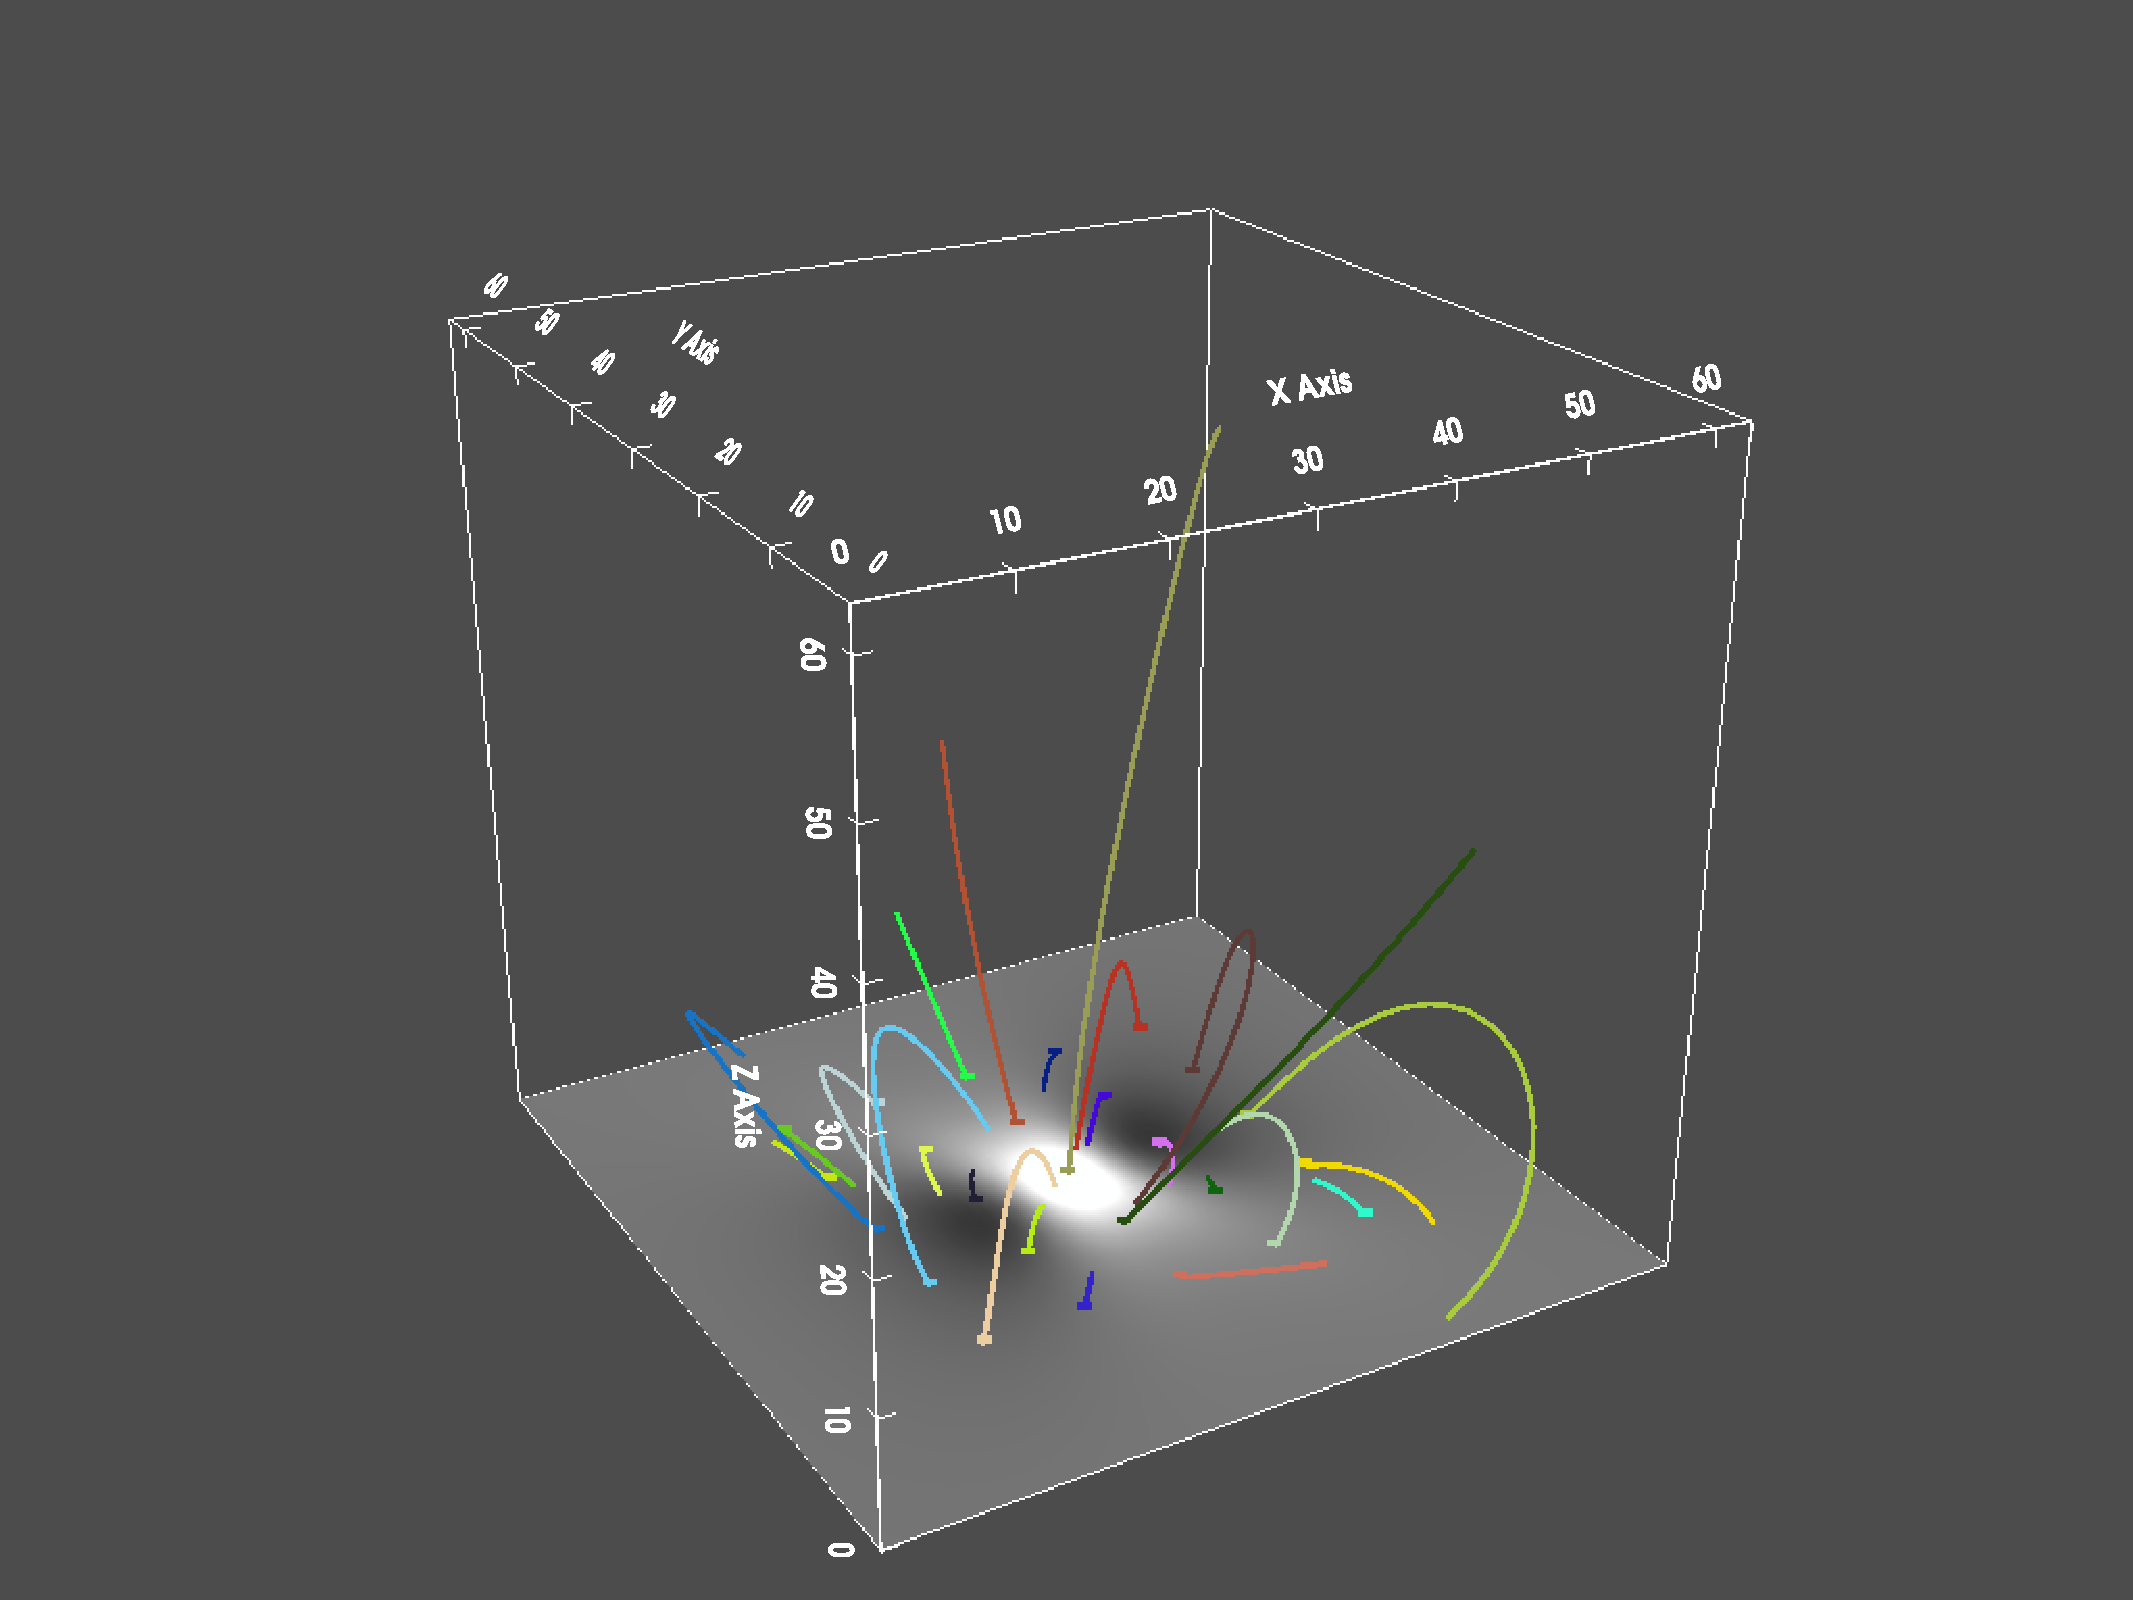
\includegraphics[trim={6cm 0cm 6cm 3cm}, clip, width=\linewidth]{"img/LL_xz_tilted.pdf"}
  \end{subfigure}
  
  \caption{The magnetic fields. Each field line is distinguished by its unique color, which is determined by its footpoint at $z=0$ plane.}\label{fig:xz_tilted}
\end{figure}

% \begin{figure}[h]
%   \centering
%   \includegraphics[width=\linewidth]{img/grafiek.png}
%   \caption{Graph of the function $sin(x) \cdot sin(y)$.
%     This figure is a bitmap, but of sufficiently high quality to be acceptable.
%     Take note of the legible axes and labels.
%   }\label{a}
% \end{figure}

% \lipsum[2-4]